\documentclass[doctor,final,11pt]{iscs-thesis}
\usepackage{graphicx}
\usepackage{soul, color}
\usepackage{listings}
\lstloadlanguages{C}
\lstset{language=C}
\lstset{backgroundcolor=\color{white}}
\lstset{frame=single}
\lstset{basicstyle=\tt}
\lstset{framexleftmargin=5pt}
\lstset{keywordstyle=\bfseries\bf\color{blue}}
\lstset{otherkeywords={\#pragma,\#define}}
\usepackage{array}
\usepackage{fancybox}
\usepackage{tikz}
\usepackage{multirow}
\usepackage{amsmath}
\usepackage{url}
\def\UrlBreaks{\do\/\do-}
\usepackage{enumerate}
\usepackage{subfigure}
\usepackage{natbib}
\usepackage{multirow}
\usepackage[ruled,vlined]{algorithm2e}
\usepackage{minitoc}
% \usepackage{showframe}
% \usepackage{hyperref}
% \hypersetup{
%     colorlinks=false,
%     linktoc=all,
%     linkcolor=black,
%     citecolor=black,
% }


% \usepackage{showframe}

%-------------------
\etitle{Techniques for Enabling Highly Efficient Message Passing on Many-Core Architectures}
\jtitle{メニーコア型大規模並列計算機向けの高性能メッセージパッシング型通信技術}
%
\eauthor{Min Si}
\jauthor{思敏}
\esupervisor{Yutaka Ishikawa}
\jsupervisor{石川裕}
\supervisortitle{Professor} % Professor, etc.
% \ecoadvisor{Pavan Balaji}
% \coadvisortitleline{Computer Scientist and Group Leader \\ of Argonne National Laboratory}
\date{July 15, 2014}
%-------------------
\begin{document}
\special{papersize=8.27in,11.69in} % A4


\newcommand{\fn}[1]{{\tt #1}}
\newcommand{\farg}[1]{\textbf{\small #1}}
\newcommand{\emp}[1]{{\tt #1}}
\newcommand{\parahead}[1]{\medskip\noindent\textbf{#1}}
\newcommand{\parasubhead}[1]{\smallskip\noindent\textbf{#1}}
\newcommand{\mynote}[1]{\textcolor{red}{[#1]}}
\newcommand{\libname}{Casper}

\begin{eabstract}
Since multicore processor chips are the norm today, the only way to 
improve the performance for high end processors is to add more threads 
and cores. Many core architecture, such as Intel Xeon Phi and Blue Gene/Q, 
provides us such a massively parallel environment with dozens of cores and
hundreds of hardware threads. To efficiently utilize such architectures, 
application programmers are increasingly looking at hybrid programming 
models comprising a mixture of processes and threads (frequently called 
``MPI+X'' models). A common mode of operation for such applications 
uses multiple threads to parallelize the computation, while one of the 
threads also issues MPI operations (i.e., MPI \texttt{FUNNELED} or 
\texttt{SERIALIZED} thread-safety mode). Although such model extremely 
improves floating point performance for most applications, still 
some of them lose performance at the bottleneck of MPI communication.
This thesis focuses on exploiting the capabilities of many core 
architectures on widely used MPI implementation, in order to eliminate
the communication bottleneck and consequently achieve highly efficient 
performance for user applications.

% parallelism
Most applications implement hybrid MPI+threads model by 
utilizing OpenMP, the most prominent of the threading models used 
in scientific computing today, to parallelize their computation.
In MPI+OpenMP applications, the common \texttt{FUNNELED}\slash \texttt{SERIALIZED} 
mode is achieved, for example, by placing MPI calls in OpenMP critical 
sections or outside the OpenMP parallel regions. However, such a model 
often means that the OpenMP threads are active only during the parallel 
computation phase and idle during the MPI calls, resulting in wasted 
computational resources. Moreover, the sequential communication phase, 
which is executed by single light-weight core, may even degrade 
performance. 
In this thesis, we first focus on MPI internal parallelism. We present MT-MPI, an
internally multithreaded MPI implementation that transparently
coordinates with the threading runtime system to share idle threads
with the application. It is designed in the context of OpenMP and
requires modifications to both the MPI implementation and the OpenMP
runtime in order to share appropriate information between them. We
demonstrate the benefit of such internal parallelism for various
aspects of MPI processing, including derived datatype communication,
shared-memory communication, and network I/O operations.

% asynchronous progress
Another way to minimize the communication bottleneck is achieving 
better overlap with computation. The MPI-2 standard introduced 
one-sided communication semantics (also known as RMA) 
that allow one process to specify all communication parameters, for 
both the sending side and the receiving side. Thus, a process can 
access memory regions of other processes in the system without the target 
process explicitly needing to receive or process the message.
RMA has the potential to deliver better communication and computation 
overlap than traditional two-sided communication does, particularly on networks 
that support one-sided communication natively, such as InfiniBand or 
Cray Aries interconnects. However, the MPI standard does not guarantee that 
such communication is truly asynchronous. Thus, most MPI implementations 
require the remote target to make MPI calls to ensure progress 
on such operations. Manticore, a process-based asynchronous progress
model for MPI on many-core architectures, is the second sub-topic 
in this thesis. Manticore uses a combination of MPI-3 shared-memory
windows and PMPI-based redirection of RMA operations to assist RMA
operations that require software intervention for progress without
affecting hardware-based RMA operations.  We describe the design of Manticore 
and compare it with other approaches for asynchronous progress.
Preliminary evaluation results show that Manticore offers improved 
performance and good scalability.

\clearpage


\end{eabstract}
\begin{jabstract}
日本語です。。。
\end{jabstract}

\maketitle

\begin{acknowledge}
% I would like to thank my adviser, Prof. Yutaka Ishikawa for guiding me patiently throughout the duration of my master study.


\end{acknowledge}

\frontmatter %% 前付け
\tableofcontents % 目次
\listfigurename
\listtablename

\mainmatter %% 本文
%%%%%%%%%%%%%%%%%%%%%%%%%%%%%%%%%%%%%%%%%%%%%%%%%%%%%%%%%%%%%%%%%%%%%
\chapter{Introduction}\label{sec:intro}
%%%%%%%%%%%%%%%%%%%%%%%%%%%%%%%%%%%%%%%%%%%%%%%%%%%%%%%%%%%%%%%%%%%%%

\section{Heterogeneous Many-Core Architectures}
The previous decade, which marked the increase of compute power from
terascale (ASCI Red supercomputer, deployed at Sandia in 1996~\cite{ascired}) to
petascale (Roadrunner supercomputer, deployed at Los Alamos in 2008~\cite{roadrunner}),
passed without a significant paradigm shift: most of the performance
improvement came from making each processor faster.
But this improvement was at the cost
of using more power per processor; and, indeed, the arrival of
petaflop supercomputers coincided with processors hitting the power
wall whereby any additional increase in the power usage of a processor would
result in the processor's components melting or becoming extremely
unreliable.  Consequently, each processor can no longer become
significantly faster.
Another three orders of magnitude increase
in performance will require at least three orders of magnitude
increase in the processing components.  This can come from
more nodes, processor cores, or threads, all of which add significant
complexity to the supercomputer.
We are already beyond the traditional work-distribution paradigm of
``equal work means equal time.''  That is, on traditional
supercomputers, if we distribute the work across processors such that
each processor gets an equal amount of work, then they take an
equal amount of time to compute.  Such fundamental assumptions are
already falling apart on today's supercomputers and will continue to
collapse in future supercomputers, primarily because of the complexity
of the processor and memory architectures involved.


\section{Complex and Irregular Scientific Applications}

The issues that arise with such a paradigm shift are not just
theoretical; indeed, they are already being seen in many application
domains.  One example is in quantum chemistry simulation.
Specifically, with the widely used software NWChem~\cite{nwchem}
(developed by PNNL), the overhead of irregularity in data
communication across processors and the resulting imbalance in the
computational load dominate the cost of current simulations (e.g., the
largest simulations of NWChem spend more than 50\% time idling).  As
researchers move to much larger simulations, this imbalance is only
going to get worse.  Another example is in bioinformatics.  The Kiki
genome assembly application~\cite{kiki}, developed by Argonne, is used
in metagenomics to understand complex environments containing many
different microbiomes (e.g., soil).  Because of restrictions in
current genome sequencing hardware, the problem tends to result in a
large number of DNA fragments that need to be assembled back into
their original complete DNA chains.  This involves enormous irregular
data movement over petabytes of data and requires several days or even
months of computation.  For instance, the largest simulation done to
date was at U. Chicago, where a 2.3-terabyte sample was assembled on a
supercomputer with 18,000 cores---this simulation took 4 days to
complete and spent 99.9\% of its time idling, because of imbalance
between processing units.

\section{Motivation}

Since multicore processors have become the most common processor
architectures today, the only way to improve the performance for
high-end processors is to add more threads and cores. Many-core
architectures, such as Intel Xeon Phi and Blue Gene/Q, provide such a
massively parallel environment with dozens of cores and hundreds of
hardware threads. More and more scientific application programmers
have begun investigating ways to utilize such architecture for scaling
application performance.

Although many-core architecture can provide the enormous power of
parallel computing, application performance may still be restricted in
various ways. Two characteristics of such hardware have to be taken
into account. First, cores are designed to be simple and low frequency
for a better performance-to-energy ratio; thus, execution on a single
core could result in extreme performance degradation. Second, the
number of cores is increasing at a faster rate than other on-chip
resources (e.g., memory), potentially resulting in scalability
bottlenecks.

To better utilize such hardware resources, application programmers
have studied several approaches that provide better parallelism and
resource sharing for different scientific applications. Many of those
approaches, however, still face communication problems that may result
in performance degradation. This doctoral research aims to exploit the
capabilities of many-core architectures on the widely used
message-passing model and propose techniques for solving existing
communication problems.


\section{Contribution}

In this thesis, we focus on optimizing the
communication of the two most popular programming models used in
modern applications: a hybrid MPI+threads model and an MPI one-sided
communication model.

\vspace{0.2ex}
\noindent\textbf{Communication optimization in hybrid MPI+threads
  model}.  An increasing number of applications are looking at hybrid
programming models, frequently called ``MPI+threads,'' to allow
resources to be shared between different cores on the node. A common
mode of operation in such hybrid models involves using multiple
threads to parallelize computation within the node, but using only one
thread to issue MPI communication. Although such a mode achieves
significant improvement in floating-point computing by massive
parallelism, it also means that most of the threads are idle during
MPI calls, a situation that translates to underutilized hardware
cores. Furthermore, since MPI communication performs only on a single
lightweight core, this mode may even result in performance
degradation.

To resolve the problems in the MPI communication of hybrid model, we
present MT-MPI~\cite{mtmpi}, an internally multithreaded MPI that
transparently coordinates with the threading runtime system to share
idle threads with the application in order to parallelize MPI internal
processing such as derived datatype communication, shared-memory
communication, and network I/O operations.

\vspace{0.2ex}
\noindent\textbf{Optimization for MPI one-sided communication}.  For
applications with large memory requirements, developers start sharing
memory resources across nodes through a global shared address space
implemented by employing MPI one-sided
communication~\cite{dinan12:armci_mpi}.  The MPI-2 and MPI-3
standards~\cite{mpi30-report} introduced one-sided communication (also
known as remote memory access or RMA), which allows one process to
specify all communication parameters for both sender and receiver.
Thus a process can access memory regions of other processes in the
system without the target process explicitly needing to receive or
process the message. Although such communication semantics can
asynchronously handle communication progress and hence hide
communication overheads from computation, it is not truly asynchronous
in most MPI implementations. For example, although contiguous PUT/GET
MPI RMA communication can be implemented in hardware on RDMA-supported
networks such as InfiniBand, thus allowing the hardware to
asynchronously handle its progress semantics, complex RMA
communication such as an accumulate operation on a 3D subarray must
still be done in software within the MPI implementation.
Consequently, the operation cannot complete at the target process
without explicitly making MPI progress and thus may cause arbitrarily
long delays if the target process is busy computing outside the MPI
stack.

To resolve the problem of asynchronous progress, we propose
Casper~\cite{casper}, a process-based asynchronous progress model for
MPI one-sided communication on multicore and many-core architectures,
that keeps aside a small user-specified number of cores as background
``ghost processes'' to help asynchronous progress. The philosophy of
Casper is centered on the notion that since the number of available
cores in modern many-core systems is increasing rapidly, some of the
cores might not always be busy with computation and can be dedicated
to helping with asynchronous progress.

In summary, this Ph.D. thesis aims to enable highly efficient message
passing on many-core architectures for various kinds of scientific
applications. Two techniques are proposed to address different
communication issues existing in modern applications.  In
Sections~\ref{sec:mtmpi} and \ref{sec:casper}, we separately present
their current state and sketch the next steps.

\section{Outline}

\chapter{Background}

%%%%%%%%%%%%%%%%%%%%%%%%%%%%%%%%%%%%%%%%%%%%%%%%%%%%%%%%%%%%%%%%%%%%%%%%%%%%%
\section{Many-Core Architectures}\label{sec:back-manycore}
%%%%%%%%%%%%%%%%%%%%%%%%%%%%%%%%%%%%%%%%%%%%%%%%%%%%%%%%%%%%%%%%%%%%%%%%%%%%%

The Intel Xeon Phi architecture features a large number of CPU cores
inside a single chip.  The Xeon Phi cards run their own Linux-based
operating system and can launch full operating system processes.  In
the native mode, system calls that cannot be handled directly on the
Xeon Phi card are transparently forwarded to the host processor, which
executes them and sends the result back to the issuing process.
Although these devices also offer the possibility of running in
\emph{offload mode}, following a GPU-like approach, this mode is not
considered in our research because it does not allow the coprocessors
to run hybrid MPI + OpenMP applications.

When MPI processes are launched on a combination of multiple nodes and
adapters, these processes internally communicate with each other using
a number of mechanisms.  Processes on the same Xeon Phi card
communicate with each other using shared memory.  Processes on the
same node communicate using the PCIe peer-to-peer capabilities.  When
communicating outside the node, for some networks such as InfiniBand,
communication is performed directly without host intervention through
the PCIe root complex.

The first generation of the product released to the public, code-named
Knights Corner~\cite{knc}, features a minimum of 60 simple cores each
capable of 4 hardware threads, providing a total of 240 hardware
threads per coprocessor.  The card is equipped with 8~GB of GDDR5 RAM.
One difference between this architecture and GPU architectures is the
fully private and coherent cache provided to each processing unit:
32~KB instruction + 32~KB data L1, and 512~KB L2 (unified), offering
high data bandwidth.  Further details on the Intel Xeon Phi
architecture can be found in~\cite{mic,knc}.


%%%%%%%%%%%%%%%%%%%%%%%%%%%%%%%%%%%%%%%%%%%%%%%%%%%%%%%%%%%%%%%%%%%%%%%%%%%%%
\section{Hybrid Programming Models}\label{sec:back-hybrid}
%%%%%%%%%%%%%%%%%%%%%%%%%%%%%%%%%%%%%%%%%%%%%%%%%%%%%%%%%%%%%%%%%%%%%%%%%%%%%

In this section we introduce the different threading modes defined by MPI for
multithreaded environments. The MPI standard provides four levels of thread safety.

\begin{figure}[h]
  \vspace{-1.0ex}
  \hspace{0.05\columnwidth}
  \subfigure[FUNNELED.] {
    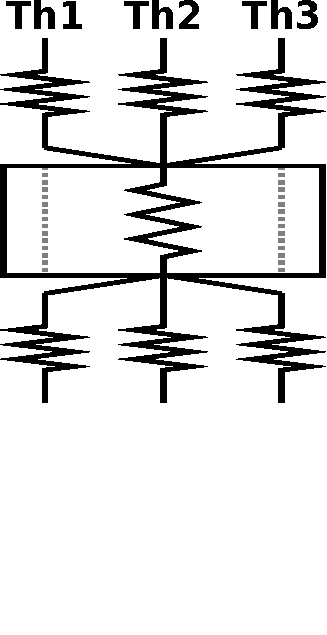
\includegraphics[width=0.26\columnwidth]{figures/mtmpi/th_funneled.pdf}
    \label{fig:th_mode_funneled}
  }
  \hspace{1.0ex}
  \subfigure[SERIALIZED.] {
    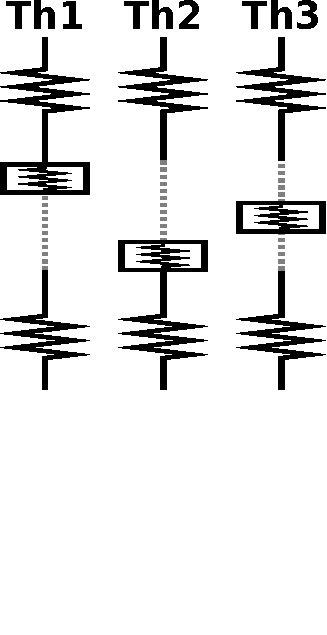
\includegraphics[width=0.26\columnwidth]{figures/mtmpi/th_serialized.pdf}
    \label{fig:th_mode_serialized}
  }
  \hspace{1.0ex}
  \subfigure[MULTIPLE.] {
    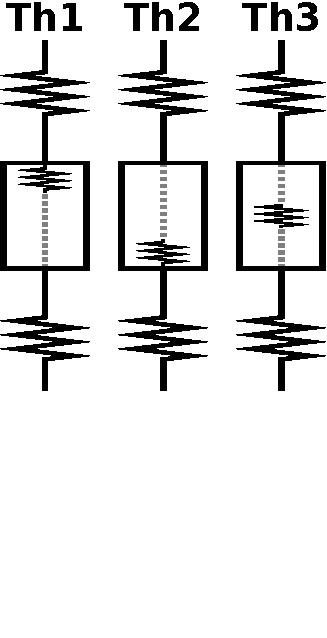
\includegraphics[width=0.26\columnwidth]{figures/mtmpi/th_multiple.pdf}
    \label{fig:th_mode_mt}
  }
  \hspace{0.05\columnwidth}
  \vspace{-2.0ex}
  \caption{Threading modes in MPI.  A line represents a thread; the
    zigzag part represents an active thread in an OpenMP region; the
    straight part represents a thread outside an OpenMP region; the
    dotted part represents an idle thread in an OpenMP region; the
    boxes represent MPI calls.}
  \label{fig:th_modes}
  \vspace{-3.0ex}
\end{figure}


\newsavebox\mpiOutsideBox
\begin{lrbox}{\mpiOutsideBox}
\begin{lstlisting}[linewidth=0.45\columnwidth]
#pragma omp parallel
{

  /* user computation */

}

MPI_Function();
\end{lstlisting}
\end{lrbox}

\newsavebox\mpiInsideMasterBox
\begin{lrbox}{\mpiInsideMasterBox}
\begin{lstlisting}[linewidth=0.45\columnwidth]
#pragma omp parallel
{
  /* user computation */
  #pragma omp master
  {
    MPI_Function();
  }
}
\end{lstlisting}
\end{lrbox}

\newsavebox\mpiInsideCriticalBox
\begin{lrbox}{\mpiInsideCriticalBox}
\begin{lstlisting}[linewidth=0.45\columnwidth]
#pragma omp parallel
{
  /* user computation */
  #pragma omp critical
  {
    MPI_Function();
  }
}
\end{lstlisting}
\end{lrbox}

\newsavebox\mpiInsideSingleBox
\begin{lrbox}{\mpiInsideSingleBox}
\begin{lstlisting}[linewidth=0.45\columnwidth]
#pragma omp parallel
{
  /* user computation */
  #pragma omp single
  {
    MPI_Function();
  }
}
\end{lstlisting}
\end{lrbox}

\begin{figure}[h]
\vspace{-1ex}
\setlength{\subfigcapskip}{5pt}
\centering
\subfigure[Outside a parallel region] {
  \usebox\mpiOutsideBox
  \label{fig:code_hybrid_outside}
}
\hfill
\subfigure[Inside omp {\tt master} region]{
  \usebox\mpiInsideMasterBox
  \label{fig:code_hybrid_master}
}
\\
\subfigure[Inside omp {\tt critical} region]{
  \usebox\mpiInsideCriticalBox
  \label{fig:code_hybrid_critical}
}
\hfill
\subfigure[Inside omp {\tt single} region] {
  \usebox\mpiInsideSingleBox
  \label{fig:code_hybrid_single}
}
\vspace{-2.0ex}
\caption{Different use cases in hybrid MPI+OpenMP.}
\vspace{-2.5ex}
\label{fig:code_omp}
\end{figure}

\vspace{1.0ex}
\noindent\textbf{MPI\_THREAD\_SINGLE.}  In this mode, a single thread
exists in the system.  This model is commonly referred to as the
MPI-only model, where a bunch of MPI processes communicate with each
other and no threads are involved.

\vspace{1.0ex}
\noindent\textbf{MPI\_THREAD\_FUNNELED.}  In this mode, multiple
th\-reads can exist, but only the master thread (the one that
initialized MPI) is allowed to make MPI calls.  Different threads can
parallelize computational phases, but all MPI communication has to be
funneled through the main thread (see
Figure~\ref{fig:th_mode_funneled}).  In typical OpenMP environments,
this involves making MPI calls either outside the OpenMP parallel
region (Figure~\ref{fig:code_hybrid_outside}) or within OpenMP master
regions (Figure~\ref{fig:code_hybrid_master}).

\vspace{1.0ex}
\noindent\textbf{MPI\_THREAD\_SERIALIZED.}  In this mode, multiple
threads can exist, and any thread can make MPI calls but only one
thread at a time.  Different threads can parallelize computational
phases, but the threads need to synchronize in order to serialize
their MPI calls (Figure~\ref{fig:th_mode_serialized}).  In typical
OpenMP environments, this involves making MPI calls within OpenMP
critical regions (Figure~\ref{fig:code_hybrid_critical}) or single
regions (Figure~\ref{fig:code_hybrid_single}).

\vspace{1.0ex}
\noindent\textbf{MPI\_THREAD\_MULTIPLE.}  In this mode, multiple
thr\-eads can exist, and any thread can make MPI calls at any time
(Figure~\ref{fig:th_mode_mt}).  The MPI implementation is responsible
for using appropriate synchronization to protect accesses to shared
internal data structures.
\vspace{1.0ex}

In this paper we focus on FUNNELED/SERIALIZED modes.


\section{Irregular Applications}

\subsection{NWChem Quantum Chemistry Application }
\subsection{SWAP-assembly Bionformatics Application}
\subsection{SWAP-assembly Bionformatics Application}
% \section{Hybrid MPI+Threads Programming}


\section{One-Sided Communication}
\chapter{Multithreaded MPI}\label{chp:mtmpi}

% \section{Introduction}\label{sec:mtmpi-intro}

Although multicore processor chips are the norm today, architectures
such as the Intel Xeon Phi take such chips to a new level of
parallelism, with dozens of cores and hundreds of hardware threads.
With the number of processing cores increasing at a faster rate than
are other resources in the system (e.g., memory), application
programmers are looking at hybrid programming models, comprising a
mixture of processes and threads, that allow resources on a node to be
shared between the different threads of a process.  In such models,
one or more threads utilize a distributed-memory programming system,
such as MPI, for their data communication.  The most prominent of the
threading models used in scientific computing today is
OpenMP~\cite{openmp}.  In OpenMP, the application developer annotates
the code with information on which statements need to be parallelized
by the compiler and the associated runtime system.  The compiler, in
turn, translates these annotations into semantic information that the
runtime system can use to schedule the computational work units on
multiple threads for parallel execution.

A common mode of operation for hybrid MPI+OpenMP applications involves
using multiple threads to parallelize the computation, while one of
the threads issues MPI operations (i.e., MPI \texttt{FUNNELED} or
\texttt{SERIALIZED} thread-safety mode).  This is achieved, for
example, by placing MPI calls in OpenMP critical sections or outside
the OpenMP parallel regions.  However, such a model often means that
the OpenMP threads are active only in the computation phase and idle
during MPI calls, resulting in wasted computational resources.  These
idle threads translate to underutilized hardware resources on
massively parallel architectures.

In this paper, we present MT-MPI, an internally multithreaded MPI
implementation that transparently coordinates with the threading
runtime system to share idle threads with the application.  We
designed MT-MPI in the context of OpenMP, which serves as a common
threading runtime system for the application and MPI.  MT-MPI employs
application idle threads to boost MPI communication and
data-processing performance and increases resource utilization.  While
the proposed techniques are generally applicable to most many-core
architectures, in this paper we focus on Intel Xeon Phi as the
architectural testbed (in ``native mode,'' where applications are
executed directly on the coprocessor).

To demonstrate the performance benefits of the proposed approach, we
modified the Intel OpenMP runtime
(http://\linebreak{}www.openmprtl.org) and the MPICH implementation
of MPI (http://www.mpich.org).  Specifically, we modified the MPI
implementation to parallelize its internal processing using a
potentially nested OpenMP parallel instantiation (i.e., one OpenMP
parallel block inside another).  We studied new algorithms for various
internal processing steps within MPI that are more ``parallelism
friendly'' for OpenMP to use.  In theory, such a model would allow
both the application and the MPI implementation to expose their
parallelism requirements to the OpenMP runtime, which in turn can
schedule them on the available computational resources.  In practice,
however, this has multiple challenges:

\begin{enumerate}
\setlength{\parskip}{-0.2ex}
\vspace{-1.2ex}

\item The modified algorithms for internal MPI processing, while
  efficient for OpenMP parallelism, are in some cases not as efficient
  for sequential processing.  Consequently, they can improve
  performance only when sufficient OpenMP parallelism is available.
  However, the actual number of threads that will be available at
  runtime is unknown.  Depending on the application's usage of
  threads, this can vary from none to all threads being available to
  MPI for processing.  Thus, if not designed carefully, the algorithms
  can perform worse than the traditional sequential implementation of
  MPI.

\item Unfortunately, the current implementation of the Intel OpenMP
  runtime does not schedule work units from nested OpenMP parallel
  regions efficiently.  It simply creates new pthreads for each nested
  parallel block and allows the operating system to schedule them on
  the available cores.  This results in creating more threads than the
  available cores, and degrading performance.

\vspace{-1.2ex}
\end{enumerate}

To work around these limitations, we modified the Intel OpenMP runtime
to expose information about the idle threads to the MPI
implementation.  The MPI implementation uses this information to
schedule its parallelization only when enough idle resources were
available.  Furthermore, such information allows the MPI
implementation to selectively choose different algorithms that trade
off between parallelism and sequential execution in order to achieve
the best performance in all cases.

We present our parallelization designs for three different parts
within the MPI implementation: (1) packing and unpacking stages
involved in derived datatype processing and communication, (2)
shared-memory data movement in intranode communication, and (3)
network I/O operations on InfiniBand.  We also present a thorough
experimental evaluation, validation, and analysis using a variety of
micro- and macrokernels, including 3D halo exchanges, NAS MG
benchmark, and the Graph500 benchmark~\cite{graph500}.

%%%%%%%%%%%%%%%%%%%%%%%%%%%%%%%%%%%%%%%%%%%%%%%%%%%%%%%%%%%%%%%%%%%%%%%%%%%%%%
\vspace{-2.0ex}
\section{Design and Implementation}\label{sec:des_and_impl}
%%%%%%%%%%%%%%%%%%%%%%%%%%%%%%%%%%%%%%%%%%%%%%%%%%%%%%%%%%%%%%%%%%%%%%%%%%%%%%

In this section we describe the design of MT-MPI, including
modifications to the MPICH implementation of MPI (v3.0.4) and the
Intel OpenMP runtime (version 20130412).


%%%%%%%%%%%%%%%%%%%%%%%%%%%%%%%%%%%%%%%%%%%%%%%%%%%%%%%%%%%%%%%%%%%%%%%%%%%%%%
\subsection{OpenMP Runtime}\label{sec:des-openmp}
%%%%%%%%%%%%%%%%%%%%%%%%%%%%%%%%%%%%%%%%%%%%%%%%%%%%%%%%%%%%%%%%%%%%%%%%%%%%%%

As described in Section~\ref{sec:intro}, for MPI to share OpenMP
parallelism with the application, two challenges need to be addressed.
The first is the different MPI internal algorithms that trade off
between parallelism and faster sequential execution.  The second is
the behavior of nested parallel regions in current OpenMP
implementations, including that of the Intel OpenMP runtime that is
used on Xeon Phi architectures.  Specifically, the OpenMP runtime
creates new pthreads for each nested OpenMP region, thus creating more
threads than the available cores and degrading performance.

To handle these issues, we modified the Intel OpenMP runtime to expose
the number of idle threads to the MPI implementation.  The idea is for
the OpenMP runtime system to track how many threads are being used by
the application vs. how many threads are idle (e.g., because they are
in an OpenMP barrier or outside an OpenMP parallel region).  Then, the
OpenMP runtime can provide this information through a new runtime
function.  The expectation in this model is that MPI could query for
the number of idle threads and use this information to (1) choose the
most efficient internal parallelization algorithms and (2) use only as
many threads in the nested OpenMP region as there are idle cores, by
explicitly guiding the number of threads in OpenMP (using the
\texttt{num\_threads} clause in OpenMP).

Arguably, the second challenge described above (additional pthreads
created in nested OpenMP regions) is an issue only with the current
implementation of the Intel OpenMP runtime.  An alternative OpenMP
runtime that internally uses user-level threads
(e.g.,~\cite{olivier12:openmp_qthreads}) might not face this
challenge.  However, given that most OpenMP implementations today use
pthreads internally and that Intel OpenMP is the only formally
supported OpenMP implementation on the Xeon Phi architecture, we
consider this to be a real problem that needs to be addressed.

\vspace{-1.0ex}
\subsubsection{Exposing Idle Threads}

To expose the number of idle threads in OpenMP, we need to understand
the status of threads in the following cases.

\vspace{1.0ex}
\noindent\textbf{MPI call made outside the OpenMP parallel regions}
(Figure~\ref{fig:code_hybrid_outside}).  In this case, all threads
except the main thread are idle (often equal to
\verb@OMP_NUM_THREADS@).  Thus, we expect MPI to be able
to benefit from a large number of idle threads.

\vspace{1.0ex}
\noindent\textbf{MPI call made in an OpenMP single region}
(Figure~\ref{fig:code_hybrid_single}).  OpenMP single regions provide
an implicit barrier on exit.  Thus, we can ideally expect threads to
be available ``soon'' if the number of idle threads is queried within
an OpenMP single region.  In practice, however, not all threads might
have reached the barrier yet, for example, because there is some skew
between the threads or because they are working on a user computation.
Thus, the number of idle threads available can vary anywhere between
zero and the maximum number of threads.  We modified the OpenMP
runtime to track each thread in order to return the actual number of
idle threads.  In this case, the amount of parallelism available to
MPI is unknown in the general case.  However, for OpenMP parallel
regions where the work shared between threads is mostly balanced and
threads are reasonably synchronized, the number of idle threads is
expected to be close to the maximum number of threads.

\vspace{1.0ex}
\noindent\textbf{MPI call made in an OpenMP master region or single
  region with a nowait clause} (Figure~\ref{fig:code_hybrid_master}).
This case is similar to the previous case (single region) with the
primary difference that there is no implied barrier at the end of such
a region.  Hence, there is no natural
synchronization point for the threads.  Nevertheless, depending on how
the application is written, it is possible to have an external
synchronization point (such as a user-specified OpenMP barrier) that
would cause more idle threads to be available.  Consequently, we use a
similar solution here as in the previous case, that is, to track the
number of idle threads.  In practice, however, we do not expect too
many idle threads to be available for MPI to use in this case.

\vspace{1.0ex}
\noindent\textbf{MPI call made in an OpenMP critical region}
(Figure~\ref{fig:code_hybrid_critical}).  OpenMP critical regions
force some synchronization between threads because only one thread can
enter a critical region at a time.  While this is not quite an
implicit barrier, its behavior with respect to the availability of
threads can be similar to that of an OpenMP single region.
Specifically, when the first thread enters the OpenMP critical region,
the remaining threads can be ideally expected to be idle ``soon.''  As
discussed earlier, this is not necessarily true if the other threads
are busy with the user computation or are skewed, but it can give a
reasonable model for us to consider.  When the second thread enters
the OpenMP critical region, the first thread is no longer expected to
be idle because it has already finished executing its critical region.
Similarly, when the last thread enters the critical region, none of
the remaining threads are expected to be idle because they have all
finished executing their critical regions.  As in the previous cases,
we track the number of idle threads inside the OpenMP runtime,
although we expect that the number of idle threads would be high for
the first few threads entering the critical section and low for the
last few threads.

\vspace{1.0ex}

In some of the cases described above (e.g., single region with
nowait), utilizing the idle threads can be risky because their status
can change at any time.  For example, they might have been idle
because they were in an unrelated critical section that has now
completed.  This would cause those idle threads to become active
again, degrading performance. In our implementation, we distinguish
how many threads are ``guaranteed to be idle'' and how many are
``temporarily available at the current time.''  To understand this
distinction, we need to look into when a thread can be idle.  There
are two cases when a thread can be idle: (1) if it is waiting in a
barrier waiting for other threads in the team to arrive or (2) if it
is outside a critical section waiting to enter it.

A thread that is in a barrier is guaranteed to be idle till all other
threads in that team reach the barrier.  Thus, when a thread in that
team queries for the number of guaranteed idle threads, all the
threads that are waiting in the barrier will contribute to the
returned value.  Waiting to enter a critical section is a bit more
tricky in that a thread is guaranteed to wait only till the thread
that is already in the critical section does not exit the critical
section.  Thus, if the thread that is already in the critical section
queries for the number of guaranteed idle threads, the threads waiting
to enter the critical section will contribute to the returned value.
For all other threads, the threads waiting to enter the critical
section will not contribute to the guaranteed idle threads but will
contribute to the temporarily available threads.

Thus, the following semantics hold true for the number of guaranteed
idle threads:

\begin{enumerate}
\setlength{\parskip}{-0.2ex}
\vspace{-1.0ex}

\item It is thread-specific.  At a given point of time, depending on
  which thread is querying for the information, the returned value
  might be different (it can increase or decrease).

\item It is OpenMP-region specific.  If the querying thread enters a
  new OpenMP region (e.g., critical or single) or exits it, the
  returned value might be different (it can increase or decrease).

\item It is time-specific.  At two different points of time the
  returned value might be different (e.g., if more threads reached a
  barrier).  However, if the same thread queries for the value and it
  is in the same OpenMP region, the value can only increase, not
  decrease.

\vspace{-1.0ex}
\end{enumerate}

We modified the OpenMP runtime to keep track of which type of OpenMP
region each thread is in, in order to return both the guaranteed
number of idle threads and the number of temporarily idle threads.  We
note that our implementation treats a thread as idle only when it is
not engaged in any OpenMP activity, including OpenMP parallel loops
and OpenMP tasks.  We also note that in our implementation the
performance overhead associated with tracking whether a thread is
actively being used by the OpenMP runtime is too small to be observed
and hence is not demonstrated in this paper.


\subsubsection{Thread Scheduling for Nested Parallelism}

For well-balanced OpenMP parallel loops with little to no skew, thread
synchronizations such as barriers are often short-lived because
threads tend to arrive at the barrier at approximately the same time.
Thus, when a thread arrives at a barrier, if it is put to sleep while
waiting for the other threads to arrive, only to be woken up in a
short amount of time, performance is degraded because of the cost of
waking up threads from a sleep state.  To work around this situation,
the Intel OpenMP runtime does not put threads to sleep immediately
when they reach a barrier.  Instead, they spin waiting for other
threads to arrive, for a configurable amount of time:
\verb@KMP_BLOCKTIME@.  A large value for this variable would mean that
threads do not become truly idle for a long time.  While this
situation is not a concern for regular OpenMP parallel loops, it can
degrade performance for nested OpenMP parallel loops since the Intel
OpenMP runtime creates more threads than the number of cores in such
cases.  Having the primary threads spin for \verb@KMP_BLOCKTIME@ would
cause more threads to be active than the number of available cores for
that much time.

When MPI calls are outside the application OpenMP parallel region
(such as in Figure~\ref{fig:code_hybrid_single}), this is not a
concern since MPI would use the same threads as the application in its
parallel region.  When MPI calls are inside the application parallel
region, however, this would require MPI to use a nested OpenMP
parallel region.  And since the threads that arrived at the barrier
would not yield the available cores immediately, this would either
require MPI to utilize lesser parallelism by only using the idle cores
or cause thread thrashing on the available cores for
\verb@KMP_BLOCKTIME@ amount of time.  Neither solution is
ideal.

In MT-MPI, to be able to employ these resources as soon as possible,
we implemented and exposed a new function in the OpenMP runtime:
\verb@set_fast_yield@.  This function plays two roles.  First, it
forces the threads in the current team to skip the active wait during
the barrier operation and immediately yield the core.  Second, it
continuously yields the core using \verb@sched_yield@ calls instead of
simply sleeping.  We used this approach primarily because of the
overhead associated with sleep vs. that of yield.  We found that
yielding allows us to manage the cores with a much lower overhead
(about 30 $\mu$s even with 240 threads) compared with sleeping (more
than 100 $\mu$s even at 16 threads).

We note that (1) our thread scheduling optimization impacts only
those threads that are guaranteed to be idle (e.g., threads waiting in
an OpenMP barrier); (2) the fast yield setting is performed internally
inside the MPI call and reset once the internal parallelism in MPI is
complete, so future OpenMP barriers are not affected by it; and (3)
the proposed thread scheduling optimization affects only that case
when MPI uses nested OpenMP parallelism (e.g., when an MPI function
is called in an OpenMP single region) and does not affect the case
when the MPI function is called outside the OpenMP parallel region.


%%%%%%%%%%%%%%%%%%%%%%%%%%%%%%%%%%%%%%%%%%%%%%%%%%%%%%%%%%%%%%%%%%%%%%%%%%%%%%
\subsection{MPI Internal Parallelism}\label{sec:des-mpi}
%%%%%%%%%%%%%%%%%%%%%%%%%%%%%%%%%%%%%%%%%%%%%%%%%%%%%%%%%%%%%%%%%%%%%%%%%%%%%%

Using the information about the idle threads exposed by our extended
OpenMP runtime, the MPI implementation can schedule its internal
parallelism efficiently to obtain performance improvements. In this
section, we demonstrate the benefit of such internal parallelism for
various aspects of the MPI processing, including derived datatype
communication, shared-memory communication, and network I/O
operations.  In our MPI implementation, we utilize only those idle
thre\-ads that are guaranteed to be available.  Although here we do
not utilize temporarily available threads, one could envision cases
(e.g., short MPI operations) where they could be.  In our
implementation, when all threads are idle (e.g., when the MPI call is
outside the OpenMP parallel region), we do not specify the number of
threads to be utilized by OpenMP; instead, we let it manage such
parallelism internally.  If fewer than the maximum number of threads
is idle, however, we direct the amount of thread parallelism to use
through the \texttt{num\_threads} OpenMP clause.


%%%%%%%%%%%%%%%%%%%%%%%%%%%%%%%%%%%%%%%%%%%%%%%%%%%%%%%%%%%%%%%%%%%%%%%%%%%%%%
\subsubsection{Derived Datatype Processing}\label{sec:imp-ddt}
%%%%%%%%%%%%%%%%%%%%%%%%%%%%%%%%%%%%%%%%%%%%%%%%%%%%%%%%%%%%%%%%%%%%%%%%%%%%%%

MPI allows applications to describe noncontiguous regions of memory
using user-derived datatypes such as \textit{vector},
\textit{indexed}, and \textit{struct}.  These derived datatypes can be
used to describe arbitrarily complex data layouts to be processed by
MPI for packing/unpacking data to/from a contiguous buffer (using
\texttt{MPI\_PACK} and \texttt{MPI\_UNPACK}) or to send/receive data.
When communicating using derived datatypes, MPI implementations
typically internally pack data into contiguous buffers, communicate
these contiguous buffers, and internally unpack them into the
recipient buffer.  Halo exchanges~\cite{halo} are a well-known example
of communications that are well suited to employ derived datatypes.

The pack and unpack processing stages consist of a set of local memory
copies.  A typical implementation traverses the derived datatype tree
and copies each noncontiguous chunk of data separately.  Some
implementations of MPI optimize such processing by representing the
entire datatype as a stack structure so that it can be iteratively
traversed rather than using a recursive traversal~\cite{mpi-dataloop}.
Given that each noncontiguous data chunk is copied to a different
location and there are no dependencies among the different data
elements, such copies are a good candidate for OpenMP parallelization.
Moreover, thanks to the relatively large private caches per core on
the Xeon Phi architecture, concurrent accesses to separate memory
regions by the different threads are expected to be highly efficient.
Therefore, we modified the MPI implementation to parallelize the
datatype data copy using OpenMP.  We note that only the lowest level
of a nested datatype (e.g., a vector of vectors) is parallelized in
MT-MPI.

\newsavebox\codeSequentialPackBox
\begin{lrbox}{\codeSequentialPackBox}
\begin{lstlisting}[linewidth=0.44\columnwidth]
for (i=0; i<count; i++){
  *dest++ = *src;
  src += stride;
}
\end{lstlisting}
\end{lrbox}

\newsavebox\codeParallelPackBox
\begin{lrbox}{\codeParallelPackBox}
\begin{lstlisting}[linewidth=0.51\columnwidth]
#pragma omp parallel for
for (i=0; i<count; i++){
  dest[i] = src[i * stride];
}
\end{lstlisting}
\end{lrbox}

\begin{figure}[t]
\centering
\subfigure[Sequential implementation.] {
  \usebox\codeSequentialPackBox
  \label{fig:code-seq-pack}
}
\hspace{0.2ex}
\subfigure[Parallel implementation.] {
  \usebox\codeParallelPackBox
  \label{fig:code-para-pack}
}
\vspace{-1.5ex}
\caption{Sequential and parallel data packing.}
\vspace{-3.5ex}
\end{figure}

One issue that we found using MT-MPI was an unintended consequence of
the compiler vectorization.  The original data\-type copy code that is
used in MPICH is shown in Figure~\ref{fig:code-seq-pack}.  While this
code works correctly for sequential data copy, it cannot be easily
parallelized by using OpenMP because the compiler cannot understand
the constant stride of accesses used through all iterations.  We
therefore modified the code as shown in
Figure~\ref{fig:code-para-pack}.  While this new implementation makes
it easier for the compiler to understand the computation and thus
parallelize it, the implementation also makes it easier for the
compiler to vectorize the code.  This situation in itself is not a
concern.  However, the Intel compiler is inefficient in vectorizing
strided loops with large stride values when the amount of data copied
in each loop is small.  Specifically, the compiler does incorrect
prefetching in this case, causing additional cache misses and thus
losing performance.  Consequently, our modification to the code is not
always beneficial and can perform worse than the sequential
implementation when very few threads are available.  To work around
this issue, we could either disable vectorization in the parallel
implementation or explicitly choose only the parallel approach when a
sufficiently large number of threads are available.  We chose the
latter approach because vectorization is still beneficial in some
cases (e.g., when the stride is small or the copy size is large).

We note that the incorrect cache prefetching and additional cache
misses that it causes have been experimentally verified, but the
results are not shown in this paper because of space restrictions.
The issue has also been reported to Intel and has been confirmed by
their compiler team.  They are expected to fix it in a future release
of the compiler.

%%%%%%%%%%%%%%%%%%%%%%%%%%%%%%%%%%%%%%%%%%%%%%%%%%%%%%%%%%%%%%%%%%%%%%%%%%%%%%
\subsubsection{Shared-Memory Communication}\label{sec:imp-lmt}
%%%%%%%%%%%%%%%%%%%%%%%%%%%%%%%%%%%%%%%%%%%%%%%%%%%%%%%%%%%%%%%%%%%%%%%%%%%%%%

When multiple MPI processes reside on the same node, since each
process has a different virtual address space, most MPI
implementations, including MPICH, use a pipelined double-copy strategy
through shared memory for intranode communication~\cite{mpich-lmt}.
As shown in Figure~\ref{fig:shd_pipeline}, a shared-memo\-ry ring buffer
is allocated between the sender and receiver processes and divided
into multiple cells; the sender process then copies part of data into
an empty cell while the receiver process copies a full cell out.

\begin{figure}[h]
  \vspace{-2.0ex}
  \subfigure[Sequential pipelining.] {
    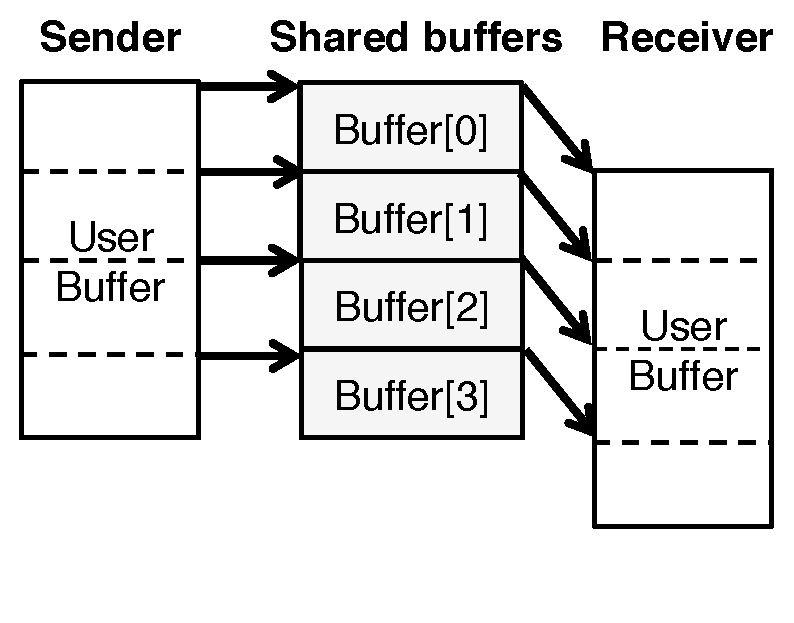
\includegraphics[width=0.43\columnwidth]{figures/mtmpi/imp-shared-pipeline.pdf}
    \label{fig:shd_pipeline}
  }
  \hfill
  \subfigure[Parallel pipelining.] {
    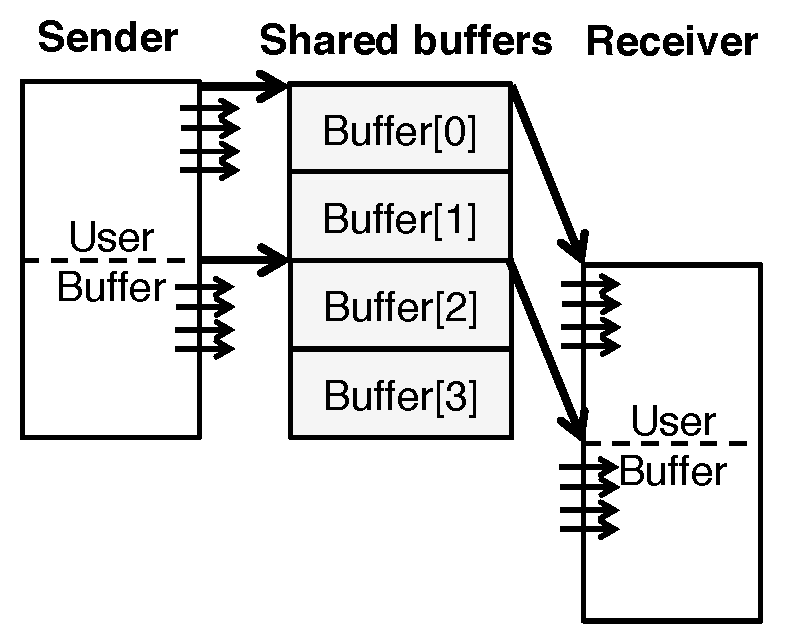
\includegraphics[width=0.43\columnwidth]{figures/mtmpi/imp-shared-parallel-pipeline.pdf}
    \label{fig:shd_parallel_pipeline}
  }
  \vspace{-2.0ex}
  \caption{Data movement of parallelization and pipelining.}
  \vspace{-2.0ex}
  \label{fig:shd_parallel_datamove}
\end{figure}

In MT-MPI, we parallelize this copy on both the sender and the
receiver side using the available idle threads.  We implemented this
optimization by extending the pipelined double-copy strategy used
within MPICH.  As shown in Figure~\ref{fig:shd_parallel_pipeline}, in
our approach we reserve multiple contiguous available cells and
concurrently copy data from the user buffer to these cells on the
sender side and from the cells to the user buffer on the receiver
side.  For messages larger than what can be held in the reserved
cells, additional pipelining is used, similar to the sequential case.
Compared with the sequential pipelining algorithm, however, the
parallel algorithm can degrade performance in the following cases.

\vspace{1.0ex}
\noindent\textbf{Small messages.}  When the message size is small,
there is not enough work in MPI to be parallelized.  In such cases,
the thread management and synchronization within OpenMP are more
expensive than the sequential copy mechanism already used in MPICH.
Thus, in this case we do not expect any performance benefit from
parallelization.

\vspace{1.0ex}
\noindent\textbf{Large messages but few idle threads.}  In our
parallel implementation, we reserve as many shared-memory cells as
possible and parallelize the copy using all of the available idle
threads.  Thus the receiver process now has to wait until data is
filled into all of the reserved cells before it can start its data
copy out of shared memory.  This approach, in essence, increases the
pipeline unit to a much larger size.  Thus, while parallelism can
improve the performance of each memory copy operation, it can also
hurt the data copy pipeline.  We note that we cannot simply reduce the
size of each shared-memory cell or the maximum number of cells
reserved to work around this issue because that would reduce the
amount of work done by each thread, thus causing the thread management
overhead to dominate.  This trend is illustrated in
Figure~\ref{fig:shd_timing}.  Specifically, compared with sequential
pipelining (Figure~\ref{fig:shd_pipeline_timing}), when the number of
threads available to MPI is small, the parallel copy does not improve
performance much but delays the receiver process from getting started
with its copy (Figure~\ref{fig:shd_poor_para_timing}).  On the other
hand, when a large number of threads are available to MPI, the parallel
copy is significantly faster, thus balancing the loss of performance
due to the reduced pipelining (Figure~\ref{fig:shd_para_timing}).

\begin{figure}
  \subfigure[Sequential pipelining.]{
  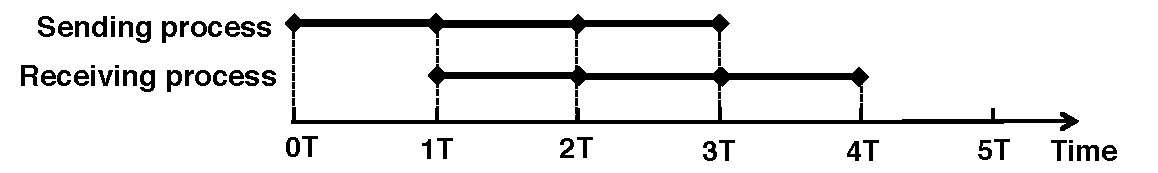
\includegraphics[width=0.95\columnwidth]{figures/mtmpi/imp-shared-pipeline-timing.pdf}
  \label{fig:shd_pipeline_timing}
  }
  \subfigure[Poor parallelism.]{
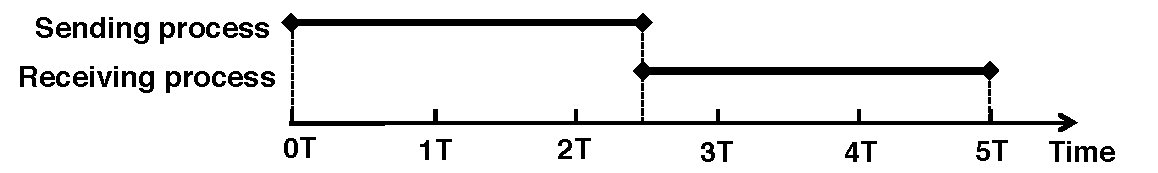
\includegraphics[width=0.95\columnwidth]{figures/mtmpi/imp-shared-poor-para-timing.pdf}
  \label{fig:shd_poor_para_timing}
  }
  \subfigure[Strong parallelism.]{
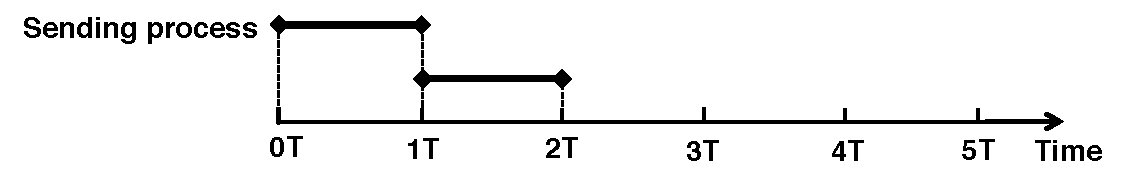
\includegraphics[width=0.95\columnwidth]{figures/mtmpi/imp-shared-para-timing.pdf}
  \label{fig:shd_para_timing}
  }
  \vspace{-2.0ex}
  \caption{Sequential pipelining vs. parallel data copy.}
  \vspace{-3.0ex}
  \label{fig:shd_timing}
\end{figure}

\vspace{1.0ex}
\noindent\textbf{Few shared-memory cells.}  The amount of data to be
copied is decided not just on the number of available threads but also
on the number of available shared-memory cells.  Specifically, during
the communication process, some cells might be in use for transferring
previous messages (or previous parts of the same message).  In such
cases, there is not enough work to be parallelized, and hence the
thread management would add too much overhead to justify the
performance improvement through parallelization.
\vspace{1.0ex}

In summary, parallelism would improve performance only when (1) the
message size is not too small ($\ge$ 64~Kbytes), (2) the number of
threads is not too few ($\ge$ 8), and (3) the total size of free cells
is not too small ($\ge$ 64~Kbytes). In our implementation, we utilize
the parallel shared-memory communication algorithm only when all three
conditions are met; otherwise we fall back to the original sequential
algorithm.  We note that the above-mentioned thresholds are
empirically evaluated on our test platform and must be tuned for
different platforms.


%%%%%%%%%%%%%%%%%%%%%%%%%%%%%%%%%%%%%%%%%%%%%%%%%%%%%%%%%%%%%%%%%%%%%%%%%%%%%%
\subsubsection{Optimizations for the InfiniBand Network}\label{sec:imp-netmod}
%%%%%%%%%%%%%%%%%%%%%%%%%%%%%%%%%%%%%%%%%%%%%%%%%%%%%%%%%%%%%%%%%%%%%%%%%%%%%%

Several MPI implementations are optimized for a variety of networks
through a layered software architecture where one of the layers
provides network-specific functionality.  In MPICH, this layer is
called the \texttt{netmod layer}.  Multiple netmod implementations
exist for MPICH over InfiniBand (IB), with more-or-less similar
functionality and performance.  In this paper we utilize the
implementation described in~\cite{mpich-ibnetmod}.

An MPI implementation utilizing IB needs to create and manage a number
of objects, including contexts, protection domains (PDs), queue pairs
(QPs), and completion queues (CQs).  A process can create one or more
IB contexts, each of which maintains a collection of state information
associated with the communication.  Each context can contain one or
more PDs, each of which defines the protection semantics of memory and
other objects used by the program, for example to allow different
connections access to different sets of memory regions.  Within a PD,
the program can create one or more QPs, each of which consists of a
send queue and a receive queue.  A QP is used to communicate between a
pair of processes.  A PD can also have one or more CQs, each of which
is used to check for the completion of communication operations on one
or more QPs.  IB also provides shared queues for better memory
management, but for simplicity we do not describe them here.

The IB software stack~\cite{ofed} is thread-safe.  When multiple
threads access the same QP or CQ, it internally uses mutexes to
maintain state consistency.  Such state consistency is expensive,
however, and can degrade performance.  Therefore, in our approach we
try to avoid such usage and instead have different threads manage
different QPs in order to maximize performance.  Even with this
approach some shared data structures still need to be protected.  To
understand how much performance improvement MPI can gain by
parallelizing the posting of network operations, we studied how much
potential parallelism there is in the IB stack that can theoretically
be exploited.  We modified the {\tt ib\_write\_bw} benchmark from the
OpenFabrics Enterprise Distribution (OFED) package~\cite{ofed} to
measure the multithreaded point-to-point IB RDMA write bandwidth
between two Intel Xeon Phi coprocessors on different nodes.  We define
three parallelism levels:

\vspace{1.0ex}
\noindent\textbf{IB contexts.}  Each process has 64 IB contexts, and
each context has one QP and one CQ.  Each thread handles operations on
a different context, CQ and QP.

\vspace{1.0ex}
\noindent\textbf{QPs and CQs.}  Each process has a single IB context
with 64 QPs and 64 CQs.  Each CQ is dedicated to a different QP.  Each
thread handles operations on different QPs and CQs, but they all share
the same context.

\vspace{1.0ex}
\noindent\textbf{QPs only.}  Each process has a single IB context with
64 QPs and one shared CQ.  Each thread handles operations on different
QPs, but they all share the same context and CQ.

\begin{figure}[h]
\vspace{-2.0ex}
\centering
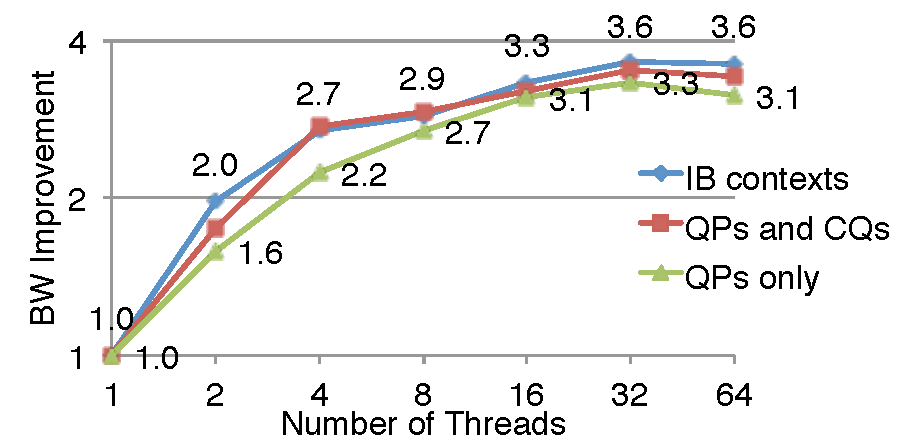
\includegraphics[width=0.8\columnwidth]{figures/mtmpi/imp-stp-ib-write-bw.pdf}
\vspace{-2.0ex}
\caption{Small (64-byte) IB RDMA write bandwidth.}
\label{fig:imp-ib-write-bw}
\vspace{-2.0ex}
\end{figure}

Figure~\ref{fig:imp-ib-write-bw} compares the communication bandwidth
of small messages (64 bytes) for the cited parallelism levels.  We
make two primary observations from the figure.  The first is that the
performance improvement with increasing threads is higher when the
number of shared resources is less.  For example, when each thread has
a separate context (\texttt{IB contexts}), with increasing threads,
the parallel performance is 3.6-fold higher than the sequential
performance.  But when the context and the CQ are shared by all
threads (\texttt{QPs only}), the parallel performance is only 3.1-fold
higher than the sequential performance.  This result is expected
because more sharing typically means more critical sections and hence
more serialization.  The second observation is that the maximum
parallelism that the IB-stack can provide is 3.6-fold when all
resources are dedicated per thread and 3.1-fold when the context and
CQ are shared between all the threads.  Most MPI implementations are
increasingly moving toward more shared resources (i.e., closer to
\texttt{QPs only}) in order to manage the per-process resource usage.
Thus, in current MPI implementations, 3.1-fold improvement is the
maximum benefit that we can expect even in the ideal case.

In MT-MPI, each QP is managed by a single thread; multiple QPs might
be managed by a single thread, but a single QP is never managed by
multiple threads.  This strategy minimizes the mutexes that the IB
stack needs to do.  We also ensure that the number of threads used for
parallelism is never more than the number of QPs, in order to minimize
thread synchronization overheads.

We note that in the MPICH IB netmod, small-message communication
employs temporary buffers that are preregistered with the network.
Since the network can communicate only to/from preregistered buffers,
user data needs to be copied into these buffers on the sender side and
out of these buffers on the receiver side.  Each connection uses a
separate QP and preregistered buffers, so the data copies on the send
and receive side are also part of the parallelism and are executed
concurrently by different threads.

Despite the potential for parallelism on many-core architectures,
several factors limit the practical parallelism
achievable in the MPI implementation.  For example, in order to
achieve the best parallelism, the MPI implementation can benefit from
a large number of operations to be issued to the network, which can be
evenly shared between the available threads.  However, such ideal
conditions are hampered by several practical restrictions in current
IB network stacks and applications.  For example, the number of
operations that can be issued to a QP or to the shared CQ is limited.
While the QP or CQ can be configured to allow for a large number of
operations, such configuration causes (sometimes large) performance
degradation due to the internal bookkeeping associated with these data
structures within the IB stack.  Consequently, the MPICH IB netmod
configures this limit to 1,024 for QPs and 32,768 for CQs, thus
forcing the maximum number of network operations each thread can post
to 1,024 and the maximum number of network operations posted across
all threads to 32,768, before thread synchronization is needed.  A
similar parallelism-limiting factor is the number of preregistered
buffers available at the sender and receiver side.

Still another parallelism constraint comes from the application
characteristics.  Specifically, since in MT-MPI we exploit parallelism
at the granularity of a QP, for ideal parallelism we need the same
amount of work per QP---a process should have close to uniform
communication with its peer processes.  In practice, however, this
assumption does not hold; indeed, the amount of communication can vary
dramatically between different processes, thus limiting the available
parallelism.

%%%%%%%%%%%%%%%%%%%%%%%%%%%%%%%%%%%%%%%%%%%%%%%%%%%%%%%%%%%%%%%%%%%%%%%%%%%%%%
\section{Evaluation and Analysis}\label{sec:mtmpi-eva}
%%%%%%%%%%%%%%%%%%%%%%%%%%%%%%%%%%%%%%%%%%%%%%%%%%%%%%%%%%%%%%%%%%%%%%%%%%%%%%

In this section, we evaluate the various techniques designed within
MT-MPI.  All our experiments are executed on the Stam\-pede
supercomputer at the Texas Advanced Computing Center
(https://www.tacc.utexas.edu/stampede/). S\-tampede consists of 6400
Dell Zeus C8220z compute nodes, each with two Xeon E5-2680 processors
and 32~GB RAM, and an Intel Xeon Phi SE10P coprocessor with 8~GB of
on-board RAM connected by an x16 PCIe 2.0 interconnect.  The nodes are
interconnected by a Mellanox FDR InfiniBand network.  All our
experiments are executed on the Xeon Phi coprocessor, with every MPI
process running on a separate coprocessor.


%%%%%%%%%%%%%%%%%%%%%%%%%%%%%%%%%%%%%%%%%%%%%%%%%%%%%%%%%%%%%%%%%%%%%%%%%%%%%%
\subsection{Derived Datatype Processing}\label{sec:eva-ddt}
%%%%%%%%%%%%%%%%%%%%%%%%%%%%%%%%%%%%%%%%%%%%%%%%%%%%%%%%%%%%%%%%%%%%%%%%%%%%%%

In this section, we describe three types of experiments that stress
derived datatype processing to various degrees: (1) derived datatype
packing performance, (2) halo data exchange with derived datatypes,
and (3) the NAS multigrid benchmark. It is noted that we use a similar
for loop for the sequential and parallel version in our comparison. It
allows us to have a fair comparison where both modes are vectorizable,
and both modes have the same issue with prefetching as described in
Section~\ref{sec:imp-ddt}. Thus, the improvement shown will be solely
due to parallelization.

\subsubsection{Derived Datatype Packing}

In our experiments with derived datatype packing (using
\texttt{MPI\_PACK}), we utilized a 3D matrix of doubles, with the X
dimension as the leading dimension.  The matrix volume was fixed at
1~GB, so increasing one dimension would reduce another.  Our
experiments involved packing different 2D planes of the 3D matrix.

\begin{figure}
\begin{center}
\subfigure[Packing the top surface with varying Z dimension.]{
  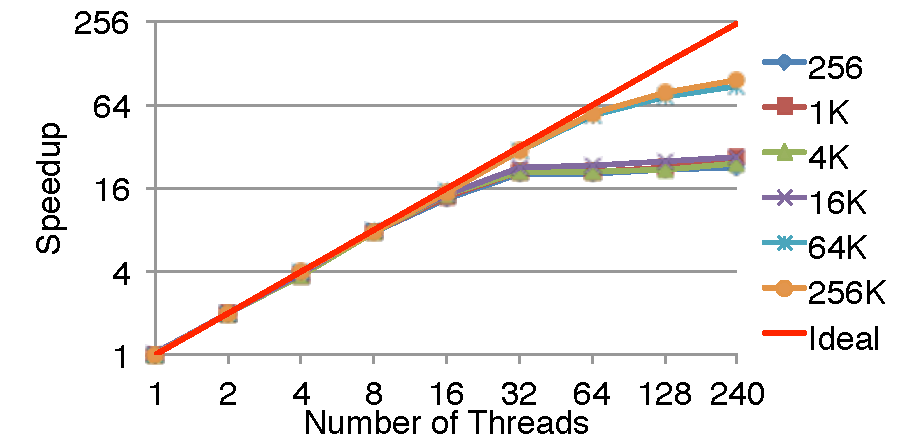
\includegraphics[width=0.8\columnwidth ]{figures/mtmpi/eva-stp-pack-3d-n.pdf}
  \label{fig:eva-pack-3d-n}
}
\subfigure[Packing the left surface with varying Y dimension.]{
  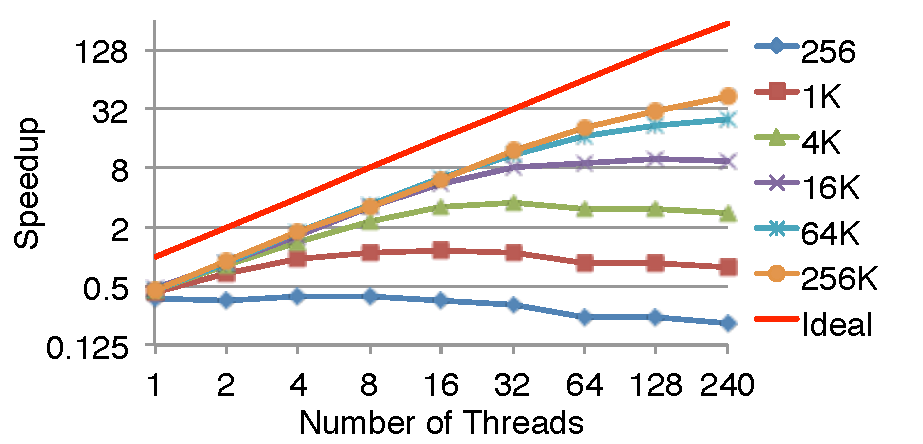
\includegraphics[width=0.8\columnwidth ]{figures/mtmpi/eva-stp-pack-3d-w.pdf}
  \vspace{-2.0ex}
  \label{fig:eva-pack-3d-w}
}
\end{center}
\vspace{-5.0ex}
\caption{Performance of parallel 3D packing.}
\vspace{-3.0ex}
\label{fig:eva-pack-3d}
\end{figure}

Figure~\ref{fig:eva-pack-3d-n} shows the performance improvement while
pac\-king the top surface (X-Z plane).  A vector datatype is utilized in
this case, with a block length equal to the length of the X dimension
and stride equal to the area of the X-Y plane; the Z dimension
indicates the vector count.  In our experiment, the Y dimension was
fixed to 2 doubles, and the Z dimension varied as indicated on the
graph legend (X dimension was varied to maintain the matrix volume).
As can be seen in the figure, MT-MPI gets a reasonably good speedup
with increasing number of threads, achieving a 96-fold improvement
compared with the original sequential version when all 240 threads are
used.  A larger Z dimension provides better speedup because that leads
to a larger iteration count for the contiguous copies and hence more
parallelism that can be exploited by MT-MPI.

Figure~\ref{fig:eva-pack-3d-w} shows the performance improvement while
pac\-king the left surface (Y-Z plane).  A two-level datatype comprising
a vector of vectors is utilized in this experiment.  The X dimension
was fixed to 2 doubles, and the Y dimension varied as indicated on the
graph legend (the Z dimension was varied to maintain the matrix
volume).  As shown in the figure, MT-MPI still achieves a relatively
good speedup compared with the sequential version (42-fold), although
less than what it achieved while packing the top surface.  This
reduction in performance is because the lowest-level vector datatype
always has a block length of one double and a count equal to the Y
dimension.  This restricts the amount of work that is done within each
iteration of the contiguous data copy operation and consequently
limits the work done by each thread, especially when the number of
iterations (i.e., the Y dimension) is small.
%   Furthermore, when the Y
% dimension is small, the parallel version is worse than the original
% sequential version (speedup is less than 1) because of the compiler's
% inefficiency in cache prefetching for vectorized code, as described in
% Section~\ref{sec:imp-ddt}.


\subsubsection{Halo Exchange of Data}

In our second set of experiments, we measured the performance of 3D
halo exchanges of data as used in stencil computations.  Both the data
and the processes are partitioned into a 3D space.  Each process
communicates with its neighboring processes with which it shares a
plane.  For our experiments we define the following four dimension
shapes for the local data on each process: (1) {\tt Cube}, with
dimensions 512 $\times$ 512 $\times$ 512 (doubles); (2) {\tt Large X},
with dimensions 16K $\times$ 128 $\times$ 64; (3) {\tt Large Y}, with
dimensions 64 $\times$ 16K $\times$ 128; and (4) {\tt Large Z}, with
dimensions 64 $\times$ 128 $\times$ 16K.  The MPI processes are evenly
distributed in all dimensions.

Figure~\ref{fig:eva-pack-3d-halo-shapes} shows the performance
improvement achieved by MT-MPI compared with the sequential version
when using 64 MPI processes.  {\tt Large Y} performs much better than
the others, delivering a 23-fold speedup with 240 threads.  To
understand this behavior, we profiled the communication time for the
different dimensions.  The halo benchmark sends data in all dimensions
simultaneously, so it is hard to profile how much time each dimension
takes.  Therefore, for profiling purposes, we modified it to serialize
communication in one dimension at a time, and we observed that
communication along the Y-Z dimension takes 85\% of the time.  While
this is obviously not entirely indicative of the true halo benchmark
that sends data in all dimensions simultaneously, it does give us some
idea of the communication cost.

As demonstrated in Figure~\ref{fig:eva-pack-3d-w}, a large Y dimension
helps improve the performance of packing in the Y-Z dimension by
providing better parallelism.  This results in a large Y impacting the
performance of the halo benchmark to the largest extent.  With {\tt
  Cube}, the Y-dimension is reduced to 512 doubles, thus reducing the
speedup to around 5.8-fold as well.  With {\tt Large X} and {\tt Large
  Z}, the Y-dimension further reduces to 128 doubles, which in turn
reduces the overall speedup to around 1.6-fold and 1.8-fold,
respectively.

\begin{figure}
\begin{center}
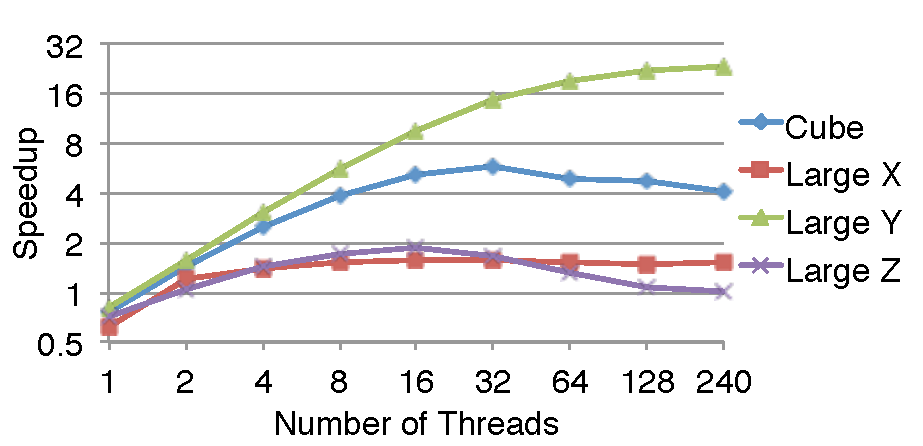
\includegraphics[width=0.8\columnwidth ]{figures/mtmpi/eva-stp-pack-3dhalo-shapes.pdf}
\vspace{-2.0ex}
\caption{3D internode halo exchange using 64 MPI processes.}
\label{fig:eva-pack-3d-halo-shapes}
\end{center}
\vspace{-5.0ex}
\end{figure}

\subsubsection{NAS Multigrid Benchmark}

\begin{figure}[t]
\begin{center}
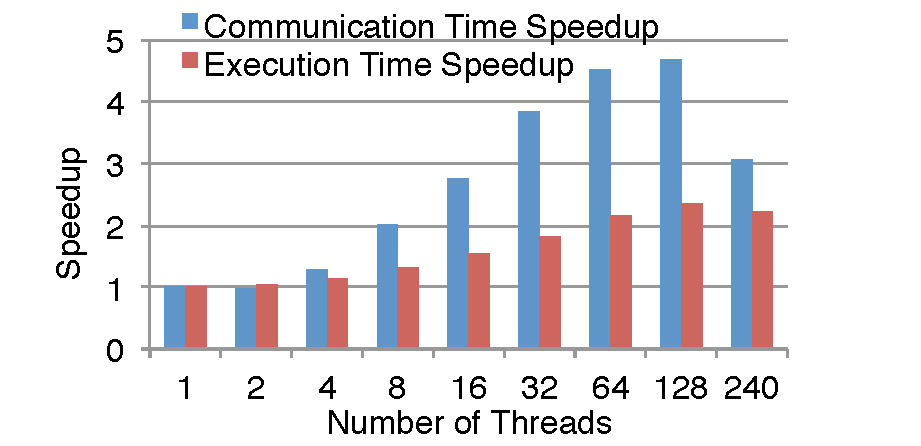
\includegraphics[width=0.8\columnwidth ]{figures/mtmpi/eva-stp-pack-mg-speedup-e.pdf}
\vspace{-2.0ex}
\caption{Hybrid MPI+OpenMP NAS MG Class E using 64 MPI processes.}
\vspace{-5.0ex}
\label{fig:eva-stp-pack-mg-sp-e}
\end{center}
\end{figure}

\begin{figure*}
\begin{center}
\subfigure[Latency.]{
  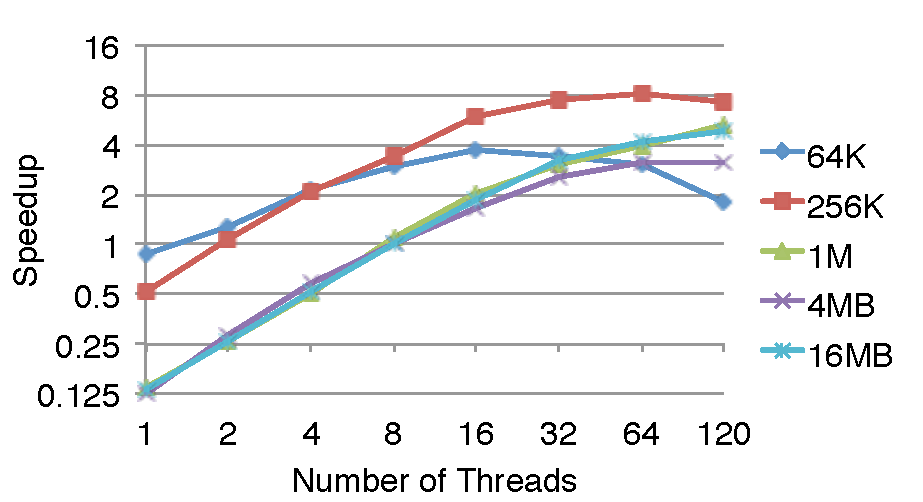
\includegraphics[width=0.63\columnwidth ]{figures/mtmpi/eva-stp-lmt-lat.pdf}
  \label{fig:eva-lmt-2m-latency}
}
\subfigure[Bandwidth.]{
  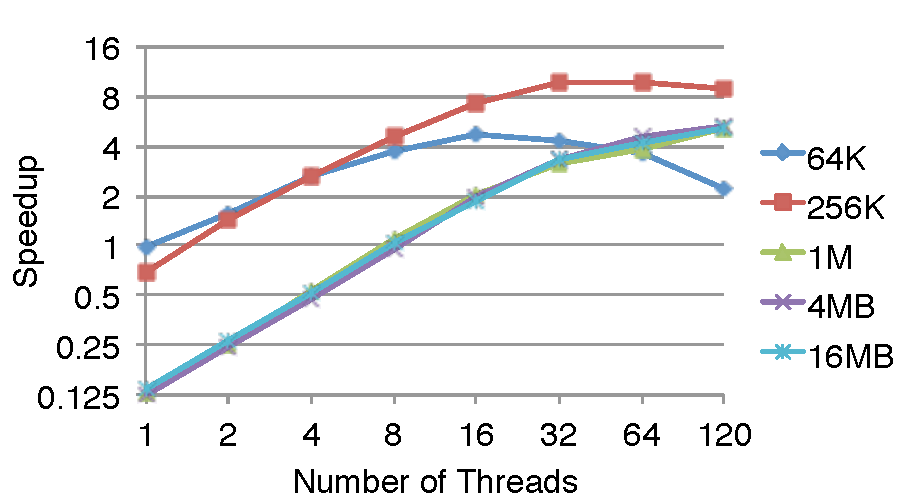
\includegraphics[width=0.63\columnwidth ]{figures/mtmpi/eva-stp-lmt-bw.pdf}
  \label{fig:eva-lmt-2m-bw}
}
\subfigure[Message rate.]{
  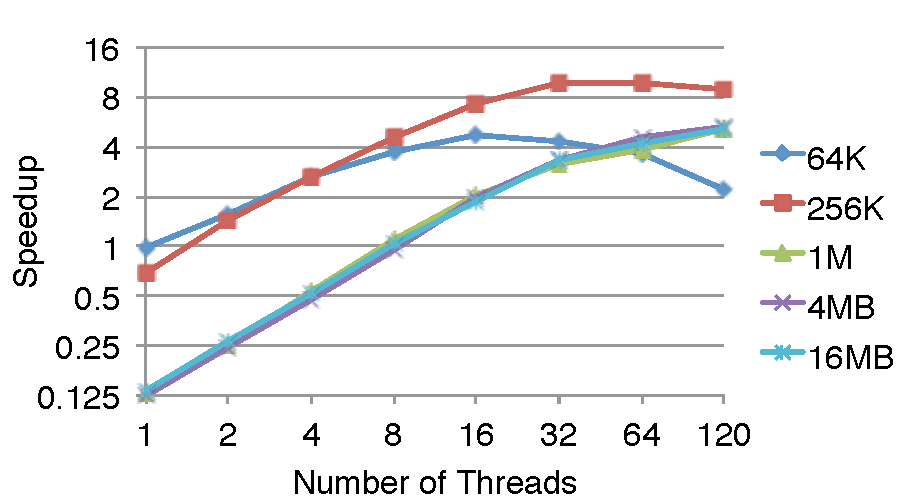
\includegraphics[width=0.63\columnwidth ]{figures/mtmpi/eva-stp-lmt-mr.pdf}
  \label{fig:eva-lmt-2m-mr}
}
\end{center}
\vspace{-5.0ex}
\caption{Shared-memory communication performance with varying message
  size between 2 MPI processes}
\vspace{-3.0ex}
\label{fig:eva-lmt}
\end{figure*}

We also evaluated a hybrid MPI+OpenMP version of the NAS Multigrid
(MG) kernel~\cite{npb} .  The original MG kernel distributed as a part
of the NAS parallel benchmarks does not contain a hybrid MPI+OpenMP
version, so we modified the MPI version to (1) parallelize the local
computation using OpenMP and (2) employ derived datatype communication
instead of manual packing.  The MG kernel implements a V-cycle
multigrid algorithm to solve a 3D discrete Poisson equation.  In every
iteration of the V-cycle routine, halo exchanges are performed with
various dimension sizes (count of double), from 2 to 514 in class E
with 64 MPI processes, and so forth.  The communication in all
dimensions except the X-Y plane is noncontiguous.

Figure~\ref{fig:eva-stp-pack-mg-sp-e} presents the speedup achieved by
MT-MPI compared with the original MPICH in class E (X, Y, Z dimension
sizes are each 2K) when employing 64 processes.  As shown in the
figure, MT-MPI helps improve the communication of MG by 4.7-fold, and
the overall execution time by 2.2-fold.  The speedup in the
communication time is still slightly lower than that of the 3D halo
exchanges with the {\tt Cube} shape shown in
Figure~\ref{fig:eva-pack-3d-halo-shapes}.  The reason is that the MG
also contains some halo exchanges with very small dimension size whose
packing process cannot be parallelized efficiently.


%%%%%%%%%%%%%%%%%%%%%%%%%%%%%%%%%%%%%%%%%%%%%%%%%%%%%%%%%%%%%%%%%%%%%%%%%%%%%%
\subsection{Shared-Memory Communication}\label{sec:eva-lmt}
%%%%%%%%%%%%%%%%%%%%%%%%%%%%%%%%%%%%%%%%%%%%%%%%%%%%%%%%%%%%%%%%%%%%%%%%%%%%%%

To measure the impact of MT-MPI on intranode shared-memory
communication, we evaluated the point-to-point communication benchmarks
in the OSU MPI microbenchmark suite version 4.1
(http://mvapich.cse.ohio-state.edu/benchm\-arks/).  In
particular, we used the latency, bandwidth, and message rate
benchmarks.  Both the original MPICH and MT-MPI use an internal
shared-memory region of 2~MB, with each cell containing 32~KB.

Figure~\ref{fig:eva-lmt} illustrates the performance of all three
benchmarks; the legends in the graph represent different message
sizes.  We notice that the performance trends of all three benchmarks
are similar, with MT-MPI delivering up to a 5-fold performance benefit
for message sizes $\ge$ 1~MB, given enough parallelism.  When the
number of idle threads is $\le$ 4, however, MT-MPI's performance is
worse than that of the original MPICH.  As discussed in
Section~\ref{sec:imp-lmt}, the reason is that MT-MPI loses some of the
pipelining capabilities in the original MPICH code in return for
thread parallelism.  But with a small number of threads, this tradeoff
is not beneficial.

Another observation we make in Figure~\ref{fig:eva-lmt} is that the
speedup of MT-MPI for message sizes 64~KB and 256~KB is much better
than that of other message sizes.  This, however, is not because of
MT-MPI's superior architecture.  Rather, it is because the
communication protocol thresholds (i.e., eager vs. rendezvous
communication thresholds) in MPICH are tuned for regular Xeon systems,
by default, and are too large for the Xeon Phi architecture.  We did
not change the default configuration of MPICH in order to avoid
introducing yet another dimension of variance in the paper.  Thus, for
64~KB and 256~KB message sizes, the original MPICH ends up using a
suboptimal communication protocol, resulting in MT-MPI's performance
falsely appearing to be significantly better as compared to other
message sizes.


%%%%%%%%%%%%%%%%%%%%%%%%%%%%%%%%%%%%%%%%%%%%%%%%%%%%%%%%%%%%%%%%%%%%%%%%%%%%%%
\subsection{InfiniBand Communication Operations}\label{sec:eva-netmod}
%%%%%%%%%%%%%%%%%%%%%%%%%%%%%%%%%%%%%%%%%%%%%%%%%%%%%%%%%%%%%%%%%%%%%%%%%%%%%%

In this section we evaluate the performance benefits achiev\-ed by
MT-MPI with our modifications to the MPICH IB netmod.  We performed two
types of experiments: (1) a one-sided communication microbenchmark
designed to demonstrate the ideal parallelism that can be obtained
within MT-MPI and (2) the one-sided version of Graph500
benchmark~\cite{graph500}.

\subsubsection{One-Sided Microbenchmark}
\label{sec:one-sided-bench}

%GWP - I suggest moving the figure from [t] to next page after fig 10, so perhaps using [h] when you do. Otherwise, fig. 11 comes before fig. 10.
\begin{figure}
\centering
\subfigure[Overall Speedup]{
  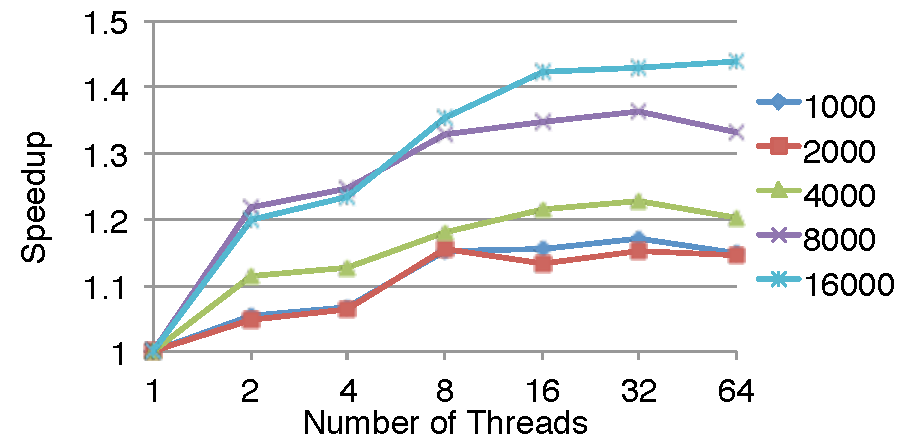
\includegraphics[width=0.8\columnwidth]{figures/mtmpi/eva-stp-ib-one2all.pdf}
  \label{fig:eva-ib-one2all}
}
\subfigure[Send Processing Speedup]{
  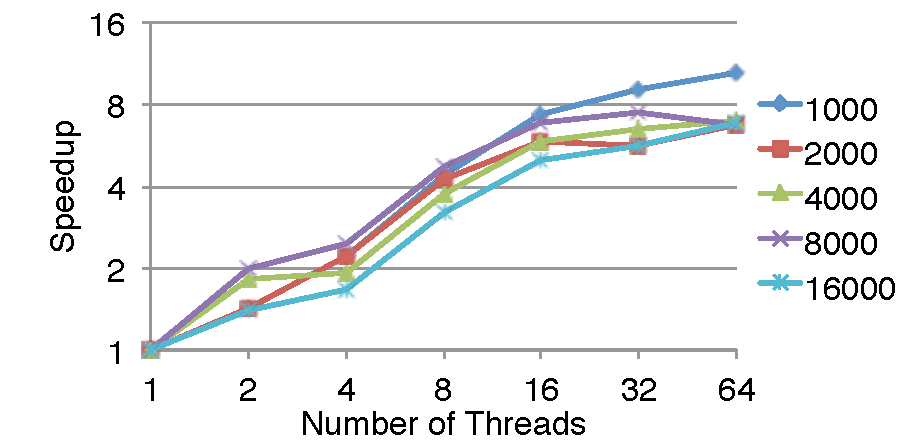
\includegraphics[width=0.8\columnwidth]{figures/mtmpi/eva-stp-ib-one2all-timing.pdf}
  \label{fig:eva-ib-one2all-timing}
}
\vspace{-2.0ex}
\caption{One-sided communication benchmark with IB using 65 MPI processes.}
\vspace{-3.0ex}
\label{fig:eva-ib-micro}
\end{figure}

We designed a microbenchmark in which one MPI process issues many {\tt
  MPI\_PUT} operations to all other processes.  Each \texttt{MPI\_PUT}
operation is for 64 bytes.  We measured the execution time of the
benchmark using 65 MPI processes; thus each process communicates with
64 other processes and internally maintains 64 IB QPs.
Figure~\ref{fig:eva-ib-one2all} shows the speedup in execution time
with MT-MPI compared with the original MPICH.  As we increase the
number of operations issued from 1,000 to 16,000, MT-MPI delivers an
increasing performance benefit, reaching a 1.44-fold speedup when
using 64 threads.

This performance benefit, however, is less than the ideal speedup of
3.1-fold that we can get by parallelizing IB communication, as
discussed in Section~\ref{sec:imp-netmod}.  To understand the reason
for this less-than-ideal speedup, we measured the execution time of
the netmod send-side communication processing at the root process
(SP), which consists only of the copy from the user buffer to a
preregistered chunk and the posting of the operations to the IB
network.  Figure~\ref{fig:eva-ib-one2all-timing} shows that the
execution time of SP delivers around 8-fold speedup when using 64
threads, which is as expected---we expect around a 3.1-fold speedup
due to the parallelization in the posting of network operations, and
some additional improvement due to the parallelized memory copy.
Table~\ref{tab:eva-ib-one2all-timing} shows the relationship between
the time spent in SP and the total execution time when issuing 16,000
operations.  Although SP shows the expected performance improvement
with MT-MPI, the percentage of time spent in SP is less than 10\% when
using more than 16 threads.  This results in a reduction in the
overall performance boost that we achieve.

\begin{table}\scriptsize
\vspace{2.0ex}
\begin{center}
\caption{Profile of the one-sided communication
  benchmark.}\label{tab:eva-ib-one2all-timing}
\vspace{-2.0ex}
\begin{tabular}{|c|ccc|cc|}
\hline
\multirow{2}{*}{Nthreads} &
\multicolumn{3}{c|}{Execution Time} &
\multicolumn{2}{c|}{Speedup} \\
\cline{2-6}
  & Total (s) & SP (s) & SP / Total ({\%}) & Total & SP \\
\hline
1 & 5.8 & 2.2 & 38 & 1 & 1 \\
4 & 4.7 & 1.3 & 27 & 1.2 & 1.7 \\
16 & 4.0 & 0.4 & 10 & 1.4 & 5.0 \\
64 & 4.0 & 0.3 & 8 & 1.4 & 6.9 \\
\hline
\end{tabular}
\end{center}
\vspace{-4.0ex}
\end{table}

\subsubsection{Graph500 Benchmark }

The second benchmark we studied was the Graph500
benc\-hmark~\cite{graph500}, which performs a breadth-first vertex-visit
operation on large graphs.  In particular, we used a scale of $2^{22}$
and an edge factor of 16 on 64 MPI processes running on different
Intel Xeon Phi coprocessors at different nodes.  In the one-sided
version of the Graph500 benchmark, every process issues many {\tt
  MPI\_Accumulate} operations to the other processes in every
breadth-first search iteration.

\begin{figure}
\centering
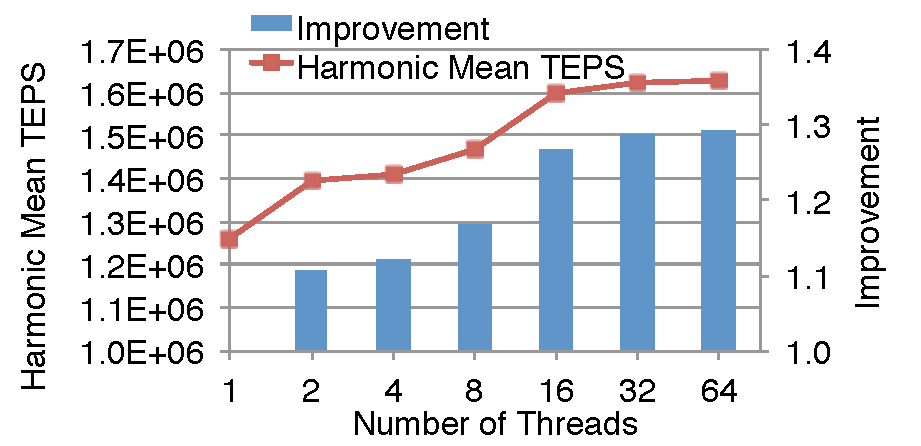
\includegraphics[width=0.8\columnwidth]{figures/mtmpi/eva-stp-ib-graph500.pdf}
\vspace{-2.0ex}
\caption{Performance of the Graph500 benchmark using 64 MPI processes.}\label{fig:eva-graph500-mean-time}
\vspace{-3.0ex}
\end{figure}

Figure~\ref{fig:eva-graph500-mean-time} shows the performance
improvement of MT-MPI compared with the original MPICH.  MT-MPI
delivers a 1.3-fold improvement in the harmonic mean of the traversed
edges per second (TEPS) when using 64 threads.  As expected, this
improvement is on par with the performance improvement we see in the
one-sided communication benchmark that we discussed in
Section~\ref{sec:one-sided-bench}.  The slightly smaller speedup
compared with the one-sided communication benchmark (which achieves a
1.44-fold speedup) is because the Graph500 benchmark does not
uniformly communicate with all peer processes, thus causing some
unevenness in MT-MPI's parallelization.



\chapter{Process-based Asynchronous Progress}\label{chp:casper}

\parahead{Note}: This chapter includes the contents that have been published in
conference papers~\cite{casper}\cite{casper-scaling}. In
reference to IEEE copyrighted material which is used with permission
in this thesis, the IEEE does not endorse any of the university of Tokyo's
products or services. Internal or personal use of this material is permitted.
If interested in reprinting/republishing IEEE copyrighted material for
advertising or promotional purposes or for creating new collective works
for resale or redistribution, please go to
\url{http://www.ieee.org/publications_standards/publications/rights/rights_link.html}
to learn how to obtain a License from RightsLink.



\section{Motivation}
% \label{sec:caspter-intro}

The MPI-2 and MPI-3 standards~\cite{mpi30-report} introduced one-sided
communication semantics (also known as remote memory access or RMA)
that allow one process to specify all communication parameters for
both the sending and receiving sides.  Thus, a process can access
memory regions of other processes in the system without the target
process explicitly needing to receive or process the message.  RMA
provides an alternative model to traditional two-sided or group
communication models and can be more natural for some applications to
use~\cite{dinan12:armci_mpi}.

While the RMA model is useful for a number of communication patterns,
the MPI standard does not guarantee that such communication is
asynchronous.  That is, an MPI implementation might require
the remote target to make MPI calls in order to ensure communication
progress to complete any RMA operations issued on it as a target.
This requirement is common in many MPI implementations.
Specifically, most network interfaces do not natively support complex
one-sided communication operations.  For example, networks such as
InfiniBand provide contiguous PUT\slash GET operations only in
hardware.  Thus, any contiguous PUT\slash GET MPI RMA communication
can be implemented almost entirely in hardware, allowing the hardware
to fully handle its progress semantics.  On the other hand, if the
application developer wants to do an accumulate operation on a 3D
subarray, for instance, such an operation must be done in software
within the MPI implementation.  Consequently, the operation cannot
complete at the target without explicit processing in software and
thus may cause arbitrarily long delays if the target process is busy
computing outside the MPI stack.

To ensure asynchronous completion of operations (i.e., ``asynchronous
progress''), traditional implementations have relied on two models.
The first is to utilize background threads~\cite{mpi2-thread}
dedicated to each MPI process in order to handle incoming messages
from other processes (e.g., used by most MPI implementations including
MPICH~\cite{mpich}, MVAPICH~\cite{mvapich}, Intel MPI~\cite{intelmpi},
and IBM MPI on Blue Gene/Q~\cite{bgq-mpi}). While this model is a
generic approach for all communication models, it has several drawbacks.
For example, it is limited with the address space sharing that the operating system
provides.  Specifically, a background thread can make progress
for only one MPI process (i.e., the process to which it belongs) and thus
requires at least as many background threads as the number of MPI
processes.  On current MPI implementations, where the MPI library
polls on the network to look for messages, this approach can waste half the
hardware threads or cores.  Furthermore, this model forces
multithreaded communication overhead on all MPI operations, which can
be expensive~\cite{thread-safety}.

The second model is to utilize hardware interrupts to awaken a kernel
thread and process the incoming RMA messages within the interrupt
context (e.g., used by Cray MPI~\cite{craympi} and IBM MPI on Blue
Gene/P~\cite[Chapter~7]{ibmmpibgp}).  While this model does not have
the large number of wasted cores or multithreaded communication
overhead of the background thread approach, it is limited in that each
message that requires target-side processing generates an interrupt,
which can be expensive.  Perhaps more fundamental, the model of
hardware interrupts is centered on the notion that all
hardware resources are busy with user computation, which needs to be
\emph{interrupted} to inject computation related to asynchronous
progress.  We believe this is not the right point of view for modern
many-core architectures where the number of cores is very large.

\section{Solution}

In this paper we present ``Casper,'' a process-based asynchronous
progress solution for MPI on multi- and many-core architectures.
An alternative to traditional thread- and interrupt-based
models, Casper provides a distinct set of benefits for applications,
 which we believe are more appropriate for large many-core
architectures.  Unlike traditional approaches, the philosophy of the
Casper architecture is centered on the notion that since the number of
cores in the system is growing rapidly, dedicating some of
the cores for helping with asynchronous progress might be better
than using an interrupt-based shared-mode model.  Similarly, the use
of processes rather than threads allows Casper to control the amount
of sharing, thus reducing thread-safety overheads associated with
multithreaded models, as well as to control the number of cores being
utilized for asynchronous progress.

The central idea of Casper is the ability of processes to share
memory by mapping a common memory object into their address spaces
by using the MPI-3 shared memory windows interface.  Specifically, Casper
keeps aside a small user-specified number of cores on a multi- or
many-core environment as ``ghost processes.''  When the application
process tries to allocate a remotely accessible memory window, Casper
intercepts the call and maps such memory into the ghost processes'
address space.  Casper then intercepts all RMA operations to the user
processes on this window and redirects them to the ghost processes
instead.

Since the user memory regions are not migrated or copied but just
mapped into the ghost processes' address space, RMA operations that
are implemented in hardware see no difference in the way they behave.
On the other hand, RMA operations that require remote software
intervention can be executed in the ghost processes' MPI stack on the
additional cores kept aside by Casper, without requiring any
intervention from the application processes.

Although the core concept of Casper is straightforward, the design and
implementation of such a framework must take several aspects into
consideration.  Most important, the framework needs to ensure that
correctness is maintained as required by the MPI-3 semantics.  While this task is
easy to manage for simple applications, the wide variety of
communication and synchronization models provided by MPI can make the task
substantially more complex for applications that are nontrivial.
This task is even more complicated for applications that use multiple
MPI-3 epoch types (e.g., passive-target and active-target) or multiple
windows of remote memory buffers because the same Casper ghost
processes need to maintain progress on all of them, thus essentially
requiring that they never indefinitely block inside an MPI operation.
Furthermore, when more than one ghost process is present, the Casper
architecture must ensure that the ordering, atomicity, and memory
consistency requirements specified by the MPI-3 standard are met in a
way that is transparent to the application.

The Casper architecture hides all this complexity from the user and
manages it internally within its runtime system.  In some
cases, however, such complexity can cause performance overhead.  In this paper
we present various techniques we used to ensure correctness while
retaining the performance of the RMA operations and enabling
low-overhead asynchronous progress.  In addition to a detailed design
of the Casper architecture, we present
experiments evaluating and analyzing Casper with various
microbenchmarks and a large quantum chemistry application.

\textbf{\em Recommended reading:} While this paper provides some
information on the MPI RMA semantics, it is not meant to be a
comprehensive description.
In order to better understand the subtle
characteristics and capabilities of MPI RMA on which this paper
relies,
we highly recommend
reading past papers and books that more
thoroughly discuss these semantics (e.g., \cite{hoefler13:mpi3-rma,
  gropp99:using-mpi-2}).

%%%%%%%%%%%%%%%%%%%%%%%%%%%%%%%%%%%%%%%%%%%%%%%%%%%%%%%%%%%%%%%%%%%%%%
\section{Casper Design Overview}\label{sec:design}
%%%%%%%%%%%%%%%%%%%%%%%%%%%%%%%%%%%%%%%%%%%%%%%%%%%%%%%%%%%%%%%%%%%%%%

Casper is designed as an external library through the PMPI
name-shifted profiling interface of MPI.  This allows Casper to
transparently link with various MPI implementations, by overloading
the necessary MPI functions.  Casper provides three primary
functionalities: (1) deployment of ghost processes to help with
asynchronous progress, (2) RMA memory allocation and setup, and (3)
redirection of RMA communication operations to appropriate ghost
processes.


%%%%%%%%%%%%%%%%%%%%%%%%%%%%%%%%%%%%%%%%%%%%%%%%%%%%
\subsection{Deployment of Ghost Processes}\label{sec:des-pe}
%%%%%%%%%%%%%%%%%%%%%%%%%%%%%%%%%%%%%%%%%%%%%%%%%%%%

Ghost processes in Casper are allocated in two steps.  In the
first step, when the user launches the application with a number of
processes, a user-defined subset of these processes is carved aside
as the ghost processes at MPI initialization time (see
Figure~\ref{fig:deg-user-comm}).  The remaining processes form their
own subcommunicator called \fn{COMM\_USER\_WORLD}.  The number of
ghost processes is user-defined through an environment variable,
allowing the user to dedicate an arbitrary number of cores on the
node for the ghost processes.

\begin{figure}[htbp]
\centering
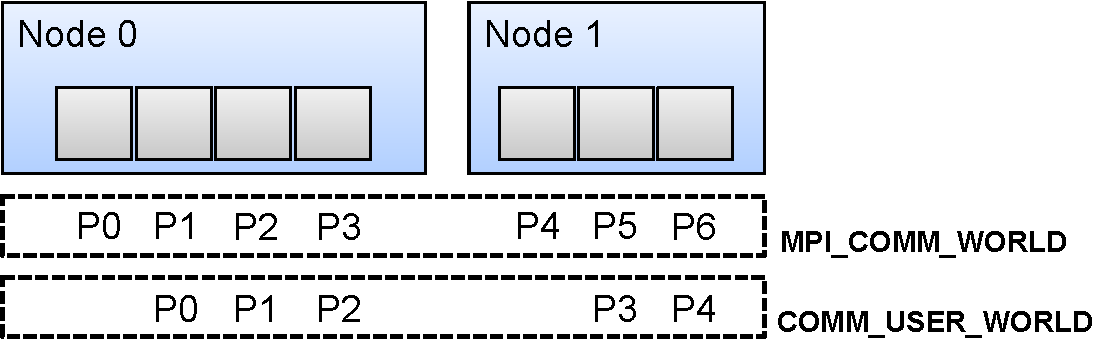
\includegraphics[width=0.9\columnwidth]{figures/casper/design_user_comm.pdf}
\caption{Casper ghost process management.}
\label{fig:deg-user-comm}
% \vspace{-1.0ex}
\end{figure}

In the second step, Casper overrides all MPI operations that take a
communicator argument and replaces any occurrence of
\fn{MPI\_COMM\_WORLD} in all non-RMA functions with
\fn{COMM\_\-USER\_WORLD} at runtime through PMPI redirection.  This
step ensures that all non-RMA communication is redirected to the
correct MPI processes, including creation of other subcommunicators
from \fn{MPI\_COMM\_WORLD}.

After initialization, ghost processes simply wait to receive any
commands from user processes in an \fn{MPI\_RECV} loop.  This approach ensures
that while the ghost processes are waiting for commands, they are
always inside the MPI runtime, thus allowing the MPI implementation to
make progress on any RMA operations that are targeted to those ghost
process.

One aspect to consider in Casper is the locality of application
buffers relative to the ghost processes.  Specifically, since a ghost
process might be depositing or reading data from the application
buffers, how far the ghost process is compared with the buffers can have
a serious impact on performance.  To handle this issue, we ensure that
the ghost processes in Casper are topology-aware.  Casper internally
detects the location of the user processes and places its ghost
processes as close to the application process memory as possible.  For
example, if a node has two NUMA domains and the user requests two
ghost processes, each of the ghost processes places itself in a
different NUMA domain and binds itself to either the process ranks or
segments in that NUMA domain.


%%%%%%%%%%%%%%%%%%%%%%%%%%%%%%%%%%%%%%%%%%%%%%%%%%%%
\subsection{RMA Memory Allocation and Setup}\label{sec:des-init}
%%%%%%%%%%%%%%%%%%%%%%%%%%%%%%%%%%%%%%%%%%%%%%%%%%%%

Remote memory allocation in the Casper architecture is tricky in that
the allocated memory must be accessible by both the application
processes and the ghost processes.  MPI provides two broad
mechanisms to declare a memory region as remotely accessible.  The
first is an ``allocate'' model (i.e., \fn{MPI\_WIN\_ALLOCATE} and
\fn{MPI\_WIN\_ALLOCATE\_SHARED}) in which MPI is responsible for creating
such memory, thus allowing the MPI implementation to optimize such
allocation (e.g., through shared memory or globally symmetric virtual
memory allocation).  The second is a ``create'' model (i.e.,
\fn{MPI\_WIN\_CREATE} and \fn{MPI\_WIN\_CREATE\_DYNAMIC}), in which
the user allocates memory (e.g., using \texttt{malloc}) and then
exposes the memory as remotely accessible.

While memory sharing between the application
processes and the ghost processes can occur in both models, doing so in the
``create'' model requires OS support to expose such capability.  This
capability is generally present on large supercomputers such as Cray
(e.g., through XPMEM~\cite{xpmem} or SMARTMAP~\cite{smartmap}) and
Blue Gene, but not always on traditional cluster platforms.  Thus, for
simplicity, we currently support only the ``allocate'' model.

When the application creates an RMA window using
\fn{MPI\_WIN\_\-ALLOCATE}, Casper follows a three-step process:

\begin{enumerate}

  \item It first allocates a shared-memory region between the user
    processes and the ghost process on the same node using the MPI-3
    \fn{MPI\_WIN\_ALLOCATE\_SHARED} function, as depicted in
    Figure~\ref{fig:deg-mem-map}.  As shown in the figure, the same
    memory region that is used by the application is also mapped onto
    the address space of the ghost process.  Thus, such memory is
    accessible through either process, although care must be taken to
    keep it consistent.

  \item Once the shared memory is allocated, it creates a number of
    internal windows using \fn{MPI\_WIN\_CREATE} to expose this memory
    to all user and ghost processes.

  \item Casper creates a new window with the same memory region
    that contains only the user processes; it then returns the new window
    handle to the application.

\end{enumerate}

\begin{figure}[tbp]
\centering
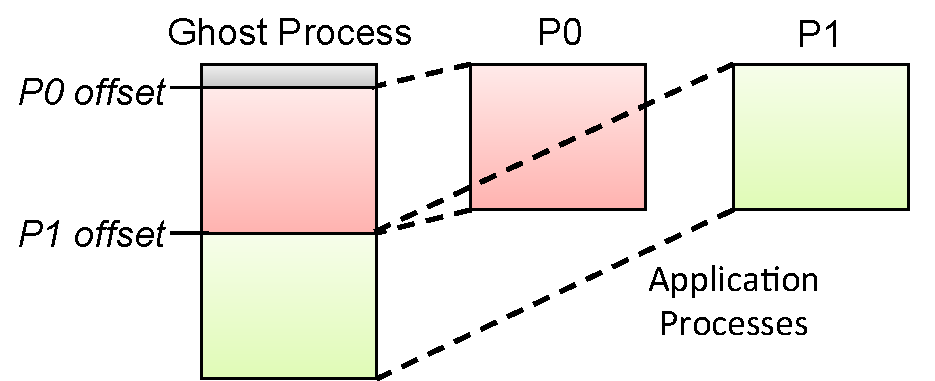
\includegraphics[width=0.7\columnwidth]{figures/casper/design_mem_map.pdf}
\caption{Casper RMA Buffer Mapping}
\label{fig:deg-mem-map}
% \vspace{-3.0ex}
\end{figure}

We note that the Casper architecture exposes the allocated
shared-memory in multiple overlapping windows.  This model provides
Casper's runtime system with enough flexibility to manage permissions
and communication aspects in a highly sophisticated manner; but at the
same time the model requires extreme caution to ensure that memory is not
corrupted and is consistent with the user's expectation.  In
Section~\ref{sec:correctness}, we describe how these internal windows
are utilized in Casper.

%% One subtle, yet important, aspect to be noted here is that the ghost
%% process allocates a slightly larger memory segment as compared to what
%% the user application requires (denoted by the grey box in
%% Figure~\ref{fig:deg-mem-map}).  This extra memory is required for
%% strict compliance with the MPI-3 standard as discussed in more detail
%% in later sections.


%%%%%%%%%%%%%%%%%%%%%%%%%%%%%%%%%%%%%%%%%%%%%%%%%%%%
\subsection{RMA Operation Redirection}\label{sec:des-op}
%%%%%%%%%%%%%%%%%%%%%%%%%%%%%%%%%%%%%%%%%%%%%%%%%%%%

Once the window becomes ready, Casper transparently redirects, through
PMPI redirection, all user RMA operations to the ghost processes on
the target node.  Such redirection needs to translate both the target
rank that the RMA operation is addressed to and the target
offset where the data needs to be written to or read from (since the
offset in the ghost process's memory region might not be the same as
the offset in the user process's memory region).  For example, based on
Figure~\ref{fig:deg-mem-map}, if an origin process does an RMA
operation at offset ``X'' of user process P1, Casper will redirect the
operation to offset ``X + P1's offset in the ghost process address
space'' on the ghost process.

When multiple ghost processes are available on the target node, Casper
attempts to utilize all of them by spreading communication operations
across them.  This approach allows the software processing required for these
operations to be divided between the different ghost processes, thus
improving performance.  Using such a model with multiple ghost processes,
however, requires extra care compared with using a model with a single ghost process. Moreover, it
raises a number of correctness issues, as we discuss
in Section~\ref{sec:multi-ghost}.

%% We note that the shared memory address space on the ghost process is
%% contiguous (see Figure~\ref{fig:deg-mem-map}).  This has both
%% advantages and disadvantages.  The advantage of the contiguous memory
%% address space comes from the offset calculation associated with
%% redirecting RMA operations.  This means that the origin needs to store
%% the offset of each potential target process in the system.  This can
%% be a scalability limitation when scaling to a large number of cores.
%% However, if all of the allocated memory was mapped to a contiguous
%% address space in the ghost process memory, for the common case where
%% all processes allocate the same amount of remotely accessible memory,
%% the origin process would only need to store one offset for each ghost
%% process, rather than one offset for each application process.  Given
%% that the number of ghost processes is expected to be much smaller than
%% the application processes, this can help with scalability concerns.
%% The disadvantage of this approach is that of false sharing.  Since the
%% bordering regions between P0's and P1's memory could be on the same
%% cache line, accesses from P0 and P1 can inadvertently result in
%% additional cache misses compared to the case where Casper was not
%% used.  In this paper, we do not study the performance implications of
%% this design choice in too much detail due to space limitations, but
%% this can be a good aspect to look at for future research.

\section{Ensuring Correctness and Performance}
\label{sec:correctness}

In this section we discuss several cases that we need to handle
inside Casper in order to maintain correctness as specified in the MPI-3
standard while achieving high performance.

With respect to performance optimizations, some of the proposed
optimizations are automatically detected and handled by the Casper
implementation, while some others are based on user hints in the form
of either \emph{info} hints or \emph{assert} hints, as specified by
the MPI standard.  Both \emph{info} and \emph{assert} hints are, in
essence, user commitments to comply with different restrictions that
allow the MPI implementation to potentially leverage different
optimizations. Specifically, \emph{info} hints are broad-sweeping and
apply to an entire window and all operations issued on that window.
Further, \emph{info} hints are extensible so each MPI implementation
can add newer hint capabilities to improve its own performance.
\emph{assert} hints, on the other hand, are more focused in scope and
typically apply to each epoch.  They are also not as easily extensible
to MPI implementation-specific hints.

The \emph{info} hints used in Casper are not
defined by the MPI-3 standard and are Casper-specific extensions.
In contrast, the \emph{assert} hints used in Casper all are MPI-3 standard defined
hints that we reuse with the same semantics as the standard.  Thus,
\emph{hints} are compatible with other MPI implementations as well,
even though some MPI implementations might not choose to take
advantage of them.

\subsection{Lock Permission Management for Shared Ghost Processes}
\label{sec:shared-ghosts}

Consider an environment where multiple application processes reside on
different cores of the same node and thus share a ghost process.  In
this case, all RMA communication to these application processes would
be funneled through the same ghost process.  In such an environment if
an origin wanted to issue an exclusive lock to more than one
application process on the same node, such a step would result in multiple
exclusive lock requests being sent from the origin to the same ghost
process.  This is disallowed by the MPI standard---an origin cannot
nest locks to the same target.  Similarly, if two origin processes
issue exclusive locks to different application processes on the same
node, this would result in multiple exclusive lock requests being sent
from different origins to the same ghost process.  While this is
correct according to the MPI standard, it would result in unnecessary serialization of all exclusive
locks to processes on the same node, thus hurting performance
significantly.

To overcome this issue, Casper internally maintains separate
overlapping windows for each user process on the node. In other words, if a
ghost process is supporting $N$ user processes, it will create $N$
overlapping windows.  Communication to the $i$th user process on each
node goes through the $i$th window.  Thus, the number of internal
overlapping windows created is equal to the maximum number of user
processes on any node of the system.  Such overlapping windows allow
Casper to carefully bypass the lock permission management in MPI when
accessing different processes but to still take advantage of them while
accessing the same process.  Since a single RMA communication
operation cannot target multiple processes at the same time, we never
run into a case where the bypassing of permission management across
processes causes an issue.

While this approach ensures correctness, it can be expensive for both
resource usage and performance.  To alleviate this concern, we allow
the user to use the info hint \texttt{epochs\_used} to specify a
comma-separated list of epoch types that the user intends to use on that
window.  The default value for this info key is all epoch types (i.e.,
``fence,pscw,lock,lockall''); but if the user sets this value to a
subset that does not include ``lock,'' Casper can use that information
to create only a single overlapping window (apart from the
user-visible window) for all its internal operations and reduce any
overhead associated with lock permission management.


%% \subsection{Self Lock Consistency}
%% \label{sec:self-lock}

%% In general, locks are nonblocking operations in that they do not need
%% to wait till the lock is actually acquired.  The MPI implementation
%% only needs to ensure that any future RMA operations are not issued to
%% the target memory before the lock is actually acquired.  Self locks
%% (i.e., when a process locks itself), however, are special in that they
%% cannot return till the lock is actually acquired.  This requirement is
%% because self locks allow applications to access their local memory
%% directly using load\slash store operations instead of MPI RMA
%% communication operations.  In such cases, the accesses are outside of
%% MPI's control and thus the MPI implementation needs to make sure to
%% acquire the lock before returning from the lock call thus forcing all
%% load\slash store operations to happen after the lock is acquired.

%% With Casper, lock operations are redirected to the ghost processes in
%% order to maintain appropriate permissions in case other origins are
%% trying to access the window at the same time.  This, however, means
%% that the lock is no longer a self-lock, but to a remote process.
%% Thus, the MPI implementation might choose to delay the lock
%% acquisition or return from the lock call before the lock acquisition
%% is complete.  At that point a process issuing load\slash store
%% operations to itself can cause data correctness issues.

%% To handle this issue, Casper performs two steps.  In the first step,
%% it issues a lock to the ghost process.  However, since the
%% acquisition of this lock might be delayed by the MPI implementation,
%% Casper internally issues an additional 1-byte GET from the window and
%% performs a flush to complete that operation.  This forced GET would,
%% in essence, block till at least the lock is acquired since the GET
%% operation cannot fetch data before the lock is acquired.  One issue
%% with this approach is that the MPI-3 standard (page 456, line 39)
%% states that data consistency is not guaranteed when a GET operation
%% and an update operation (such as a PUT or ACCUMULATE operation) occur
%% simultaneously at the same memory location.  Thus, if the user
%% application is updating the same location as the one that is being
%% fetched by the forced GET described above, data consistency is not
%% guaranteed.  Such data inconsistency makes sense for the GET operation
%% but seems to be an unnecessary restriction on the update operation,
%% i.e., the update should still be valid in such cases.  As active
%% members of the MPI Forum RMA working group, we believe this is an
%% unintended oversight and should be fixed in the upcoming MPI-3.1 or
%% MPI-4.0 standard.  However, in order to meet the strict wording of the
%% standard, we need an alternative approach.  Therefore, in Casper, we
%% allocate additional ``hidden bytes'' at the ghost process (depicted by
%% the gray box in Figure~\ref{fig:deg-mem-map}) that are not exposed to
%% the user application.  The additional force GET operation is issued on
%% these hidden bytes thus guaranteeing that it cannot cause any
%% potential corruption of user data.

%% In the second step, now that the permission issue is managed by the
%% lock at the ghost process, Casper issues a second self-lock at the
%% origin process.  This lock does not manage any permissions (since it
%% is guaranteed to be not competed), but is necessary for managing memory
%% consistency through appropriate system-specific memory barriers that
%% the MPI implementation might be required to do.

%% While the above solution maintains correctness, it clearly adds
%% additional lock acquisition overhead that can have performance
%% implications.  In order to alleviate such performance impact, we use
%% the info hint \texttt{no\_load\_store} to let the user specify when
%% she does not intend to access the local window with load/store
%% operations, i.e., all data movement to/from the remotely accessible
%% memory will be done using MPI RMA operations.  With this hint, Casper
%% would still issue the lock operation to the ghost process, but does
%% not have to force acquire it.  Furthermore, Casper can skip the second
%% self-lock completely since that is only needed for local load\slash
%% store operations.

%% The user can also use the \texttt{MPI\_MODE\_NOCHECK} assert (which is
%% already specified in the MPI-3 standard) to help in this case.  The
%% \texttt{MPI\_MODE\_NOCHECK} hint tells us that the user is
%% guaranteeing that there will be no contention on the lock and hence on
%% the access permissions to the window, thus removing the necessity for
%% the force lock for permission management.

%% As a side benefit, this hint also allows us to issue local PUT/GET
%% operations directly instead of forwarding them to the ghost process,
%% since we know that the ghost process would not be receiving any
%% conflicting epochs at the same time.  It is still possible that the
%% ghost process will receive a PUT/GET operation to the same location as
%% the local PUT/GET operations, but the MPI standard already states that
%% doing so can result in data corruption, which covers data conflicts
%% within Casper as well.  We note that we do not use this optimization
%% for accumulate-style operations since that would break the atomicity
%% constraints enforced by the MPI standard.


\subsection{Managing Multiple Ghost Processes}
\label{sec:multi-ghost}

In Casper, the user is allowed to configure a node with multiple ghost
processes.  Doing so allows better sharing of work when the number of
operations requiring such asynchronous progress is large.  However,
such a configuration requires additional processing to maintain
correctness.  A simple model in which all communication is randomly
distributed across the different ghost processes has two issues that
need to be handled: (1) lock permissions in the \emph{lock-unlock}
epoch and (2) ordering and atomicity constraints for accumulate
operations.

When the \emph{lock-unlock} epoch type is used, Casper will internally
lock all ghost processes on a node, when a lock operation for a
particular application process is issued, in the hope of spreading
communication across these ghost processes.  In practice, however,
many MPI implementations might not acquire the lock immediately, instead
delaying them to a future time (e.g., when an RMA communication operation
is issued to that target).  Given this behavior, consider an
application that simply does one \emph{lock-put-unlock}.  In this
example, Casper might randomly pick a ghost process, thus picking one
ghost process on one origin while picking a different ghost process on
another origin.  For implementations that delay lock acquisition, this
example would mean that the two ghost processes would get exclusive locks from
two different origins to access the same memory location.  Since the
lock management in MPI is unaware of the shared-memory buffers in
Casper, both exclusive locks would be granted, resulting in data
corruption.

%% \newsavebox\multiHelperIssueOrigCode
%% \begin{lrbox}{\multiHelperIssueOrigCode}
%% \begin{lstlisting}[linewidth=0.83\columnwidth]
%%   MPI_Win_lock(MPI_LOCK_EXCLUSIVE, P1, 0, win);
%%   MPI_Put(..., P1, ...);
%%   MPI_Win_unlock(P1, win);
%% \end{lstlisting}
%% \end{lrbox}
%% \newsavebox\multiHelperIssueMtCode
%% \begin{lrbox}{\multiHelperIssueMtCode}
%% \begin{lstlisting}[linewidth=0.83\columnwidth]
%%   MPI_Win_lock(MPI_LOCK_EXCLUSIVE, G1, 0, win);
%%   MPI_Win_lock(MPI_LOCK_EXCLUSIVE, G2, 0, win);

%%   /* Pick a random ghost process */
%%   G = randomly_pick_ghost();
%%   MPI_Put(..., G, ...);

%%   MPI_Win_unlock(G1, win);
%%   MPI_Win_unlock(G2, win);
%% \end{lstlisting}
%% \end{lrbox}

%% \begin{figure}
%% \begin{CenteredBox}
%% \subfigure[User code]{
%%   \usebox\multiHelperIssueOrigCode
%% }
%% \end{CenteredBox}
%% \begin{CenteredBox}
%% \subfigure[Casper translated code] {
%%   \usebox\multiHelperIssueMtCode
%% }
%% \end{CenteredBox}
%% \caption{Lock acquisitions issues with multiple ghost processes.}
%% \label{code:multi-ghost-lock-issue}
%% \vspace{-4.0ex}
%% \end{figure}

The second issue concerns the atomicity and ordering
guarantees provided by the MPI standard for concurrent accumulate
operations to the same location (see \cite{mpi30-report}, Section
11.7.1).  Each basic datatype element of concurrent accumulate
operations issued by the same or different origin processes to the
same location of a target process must be performed atomically.
Similarly, two accumulate operations from the same origin to the same
target at the same memory location are strictly ordered.  In Casper,
if a user process is served by a single ghost process, such atomicity
is already provided by the MPI implementation.  If a user
process is served by multiple ghost processes, however, they might
simultaneously be accessing the same memory region, thus breaking both
atomicity and ordering.

To address these issue, Casper uses a two-phase solution.  The first
phase is to provide a base ``static binding'' model in which each ghost
process is statically assigned to manage only a subset of the remotely
accessible memory on the node.  This model ensures correctness as per
the MPI standard but can have some performance cost.  We propose two
static binding approaches in this paper: rank binding and segment
binding.  The second phase is to identify periods in the application
execution where the issuing of some operations to ghost processes can
be done in a more dynamic fashion.  In this section, we discuss both
phases.

\subsubsection{Static Rank Binding}
With rank binding, each user process
binds to a single ghost process, and any RMA operations issued to that
user process are always directed to that ghost process.  Therefore,
different origins locking the same target are redirected to the
same ghost process, thus benefiting from MPI's internal permission
management.  Similarly, different accumulate operations targeting the
same user process are redirected to the same ghost process,
thus benefiting from MPI's internal ordering and atomicity management.
This model completely works around the problem with multiple ghost
processes since each user application process is associated with
only a single ghost process.  The disadvantage of this approach, however,
is that if the amount of communication to the different user
application processes is not uniform, one ghost process might get more
work than the others get, thus causing load imbalance.

\subsubsection{Static Segment Binding}  With segment binding, the total memory
exposed by all the processes on the node is segmented into as many
chunks as the number of ghost processes, and each chunk or segment is
bound to a single ghost process.  Thus, given a particular byte of
memory, a single ghost process ``owns'' it.  When the user application
issues a lock operation, Casper will still lock all ghost processes;
but when the actual RMA communication operation is issued, it is
redirected to the appropriate ghost processes that own that segment of
the memory.  In this model different origin
processes can get simultaneous access to the same target through
different ghost processes.  However, they cannot simultaneously update
the same memory region, thus making such shared access inconsequential
and still guaranteeing application correctness.

A second aspect that must be considered in segment binding is that
segmentation must be at a basic-datatype-level granularity in order to maintain
MPI's requirements for atomicity.  To handle this, we must ensure that
segments are divided at an alignment of the maximum size of MPI basic
datatypes (i.e., 16~bytes for \farg{MPI\_REAL}).  This alignment is needed in
order to guarantee that no basic datatype is divided between two ghost
processes.  Thus, although an operation may be divided into multiple
chunks and issued to different ghost processes, each basic datatype
unit belongs to a single chunk and is directed to a single ghost
process, thus guaranteeing atomicity and ordering.  This approach
will work in most cases since most compilers enable data alignment by
default (i.e., a double variable has to be allocated on an address
that is a multiple of eight).  Hence, it is safe to divide an
operation into different aligned segments.  We note, however, that this
approach is not strictly portable.  Compilers are allowed to not
enforce data alignment or allow users to explicitly disable structure
padding, resulting in unsafe segmentation.  Nevertheless, data
alignment is always recommended for performance; and some
architectures, such as SPARC \cite{sparc}, even require it for
correctness.

%% \begin{figure}
%% \begin{CenteredBox}
%% \begin{lstlisting}[linewidth=0.69\columnwidth]
%% struct __attribute__((__packed__)) Foo {
%%    char a;
%%    double b;
%% };
%% \end{lstlisting}
%% \end{CenteredBox}
%% \caption{Padding disabled structure.}
%% \label{code:no-padding}
%% \end{figure}

The advantage of the static segment binding model compared with the
static rank binding model is that the load on a given ghost process is
determined by the memory bytes it has access to, rather than the
process it is bound to.  In some cases, such a model can provide
better load balancing than the static rank binding model.  However,
the static segment binding model
has several disadvantages.  Most important, this solution relies on
analyzing the specific bytes on the target process that are being
accessed for each RMA operation.  For operations using contiguous
datatypes that completely fall within one data segment, this model can
be straightforward, since the operation is simply forwarded to the
appropriate ghost process.  If the data overlaps two or more
segments, however, Casper must internally divide the operation into
multiple operations issued to different ghost processes.  This
solution becomes even more complex when the data being transmitted is
noncontiguous, in which case the datatype needs to be expanded and
parsed before the segments it touches can be determined.

\subsubsection{Dynamic Binding}  In applications that have balanced
communication patterns, each target process on a compute node tends to
receive an approximately equal number of RMA operations.  The best
performance can be achieved for such patterns by equally distributing
the number of processes handled by each ghost process.  In such cases,
a static binding approach might be a good enough solution for load
balancing.  For applications with more dynamic communication
patterns, however, a more dynamic selection of ghost processes is needed, as
long as such an approach does not violate the correctness requirements
described above.

In Casper, to help with dynamic binding, we define
``static-binding-free'' intervals of time.  For example, suppose the
user application issues a lock operation to a target. This lock would
be translated to a lock operation to the corresponding ghost process to
which the target process is bound.  After issuing some RMA communication
operations, if the user application flushes the target,
the MPI implementation must wait for the lock to be acquired
and cannot delay the process of lock acquisition any further.  The period after the
flush operation has completed and before the lock is released is
considered a ``static-binding-free'' period.  That is, in this period
we know that the lock has already been acquired.  In such periods, the
Casper implementation no longer has to do lock permission management
and is free to load balance PUT/GET operations to any of the ghost
processes with the same lock type as that specified by the user
application process.  We note that this optimization is not valid for
accumulate-style operations, in order to maintain the atomicity and
ordering guarantees specified by the MPI standard.

We utilize three dynamic load-balancing approaches in Casper.  The
first is a ``random'' algorithm that randomly chooses a ghost process
from the available ghost processes for each RMA operation.  The second
is an ``operation-counting'' algorithm that chooses
the ghost process that the origin issued the least number of
operations to.  The third is a ``byte-counting'' algorithm that
chooses the ghost process that the origin issued the least number of
bytes to.


\subsection{Dealing with Multiple Simultaneous Epochs}
\label{sec:multiwin}

The MPI standard does not allow a process to simultaneously
participate in multiple overlapping epoch types on a given window.
However, for disjoint sets of processes or for the same set of
processes with different windows, no such restrictions exist.
Thus, one could imagine an application in which a few of the processes
are participating in a \emph{lock-unlock} epoch on one window, while
another disjoint set of processes is participating in a \emph{fence}
epoch on another window.  If more than one of these processes are on
the same node, the ghost processes have to manage multiple
simultaneous epochs.  The primary difficulty with handling multiple
simultaneous epochs, especially active target epochs such as
\emph{fence} and \emph{PSCW}, is that the epoch opening and closing
calls in these epochs are collective over either all or a subset of
processes in the window and these calls are blocking with no
nonblocking variants.  Thus, if a ghost process participates in one
epoch opening or closing call, it is stuck in a blocking call and hence
loses its ability to help with other epochs for other user processes.

To work around this issue, Casper converts all active-target epochs
into passive-target epochs on a separate window.  Further, it
manages permission conflicts between \emph{lockall} and \emph{lock} by
converting \emph{lockall} to a collection of \emph{lock} operations in
some cases.  The following paragraphs describe these changes in more
detail.

\subsubsection{Fence}  The \emph{fence} call supports a simple
synchronization pattern that allows a process to access data at all
processes in the window.  Specifically, a fence call completes an
epoch if it was preceded by another fence and starts an epoch if it is
followed by another fence.

In Casper, we translate \emph{fence} to a \emph{lockall-unlockall}
epoch.  Specifically, we use a separate window for \emph{fence}; and
when the window is allocated, we immediately issue a \emph{lockall}
operation.  When the user application calls \emph{fence}, we
internally translate it to \emph{flushall-barrier}, where the
\emph{flushall} call ensures the remote completion of all operations
issued by that origin and the \emph{barrier} call synchronizes
processes, thus ensuring the remote completion of all operations by all
origins.  This model ensures that the ghost processes do not need to
explicitly participate in any active target synchronization calls,
thus avoiding the blocking call issues discussed above.

While correct, this model has a few performance issues.  First, a
\emph{fence} call does not guarantee remote completion of operations.
The return of the \emph{fence} call at a process guarantees only the
%GWP is "at" a process the correct way to say this?
local completion of operations issued by that process (as an origin)
and the remote completion of operations issued to that process (as a
target).  This is a weaker guarantee than what Casper provides,
which is remote completion of all operations issued by all processes.
Casper's stricter guarantees, while correct, do cost performance, however.
Therefore, such
remote completion through \emph{flushall} can be skipped if the user
provides the \texttt{MPI\_MODE\_NOPRECEDE} assert indicating that
no operations were issued before the \emph{fence} call that need
to be flushed.

Second, an MPI implementation can choose to implement \emph{fence} in
multiple different ways.  For example, one possible implementation of
the \emph{fence} epoch is to delay all RMA communication operations to
the end of the epoch and issue them only at that time.  Thus, if the
MPI implementation knows that a \emph{fence} call does not complete any
RMA communication operations (e.g., if it is the first fence), it can
take advantage of this information to avoid synchronizing the
processes.  Casper does not have this MPI
implementation internal knowledge, however.
Thus, it always has to assume that the
MPI implementation might issue the RMA communication operations
immediately, and consequently it always has to synchronize processes.
Again, doing so costs performance.  However, if the user specifies the
\texttt{MPI\_MODE\_NOSTORE}, \texttt{MPI\_MODE\_NOPUT}, and
\texttt{MPI\_MODE\_NOPRECEDE} asserts, Casper can skip such
synchronization since there are no store operations before the
\emph{fence} and no PUT operations after the \emph{fence} that might
impact the correctness of the data.

Third, when \emph{fence} is managed by the MPI implementation, it
internally enforces memory consistency through appropriate memory
barriers.  In Casper, since the \emph{fence} call is translated to
passive-target synchronization calls, such memory consistency has to
be explicitly managed.  Thus, during each \emph{fence} call, we add
an additional call to \fn{MPI\_WIN\_SYNC} to allow such memory
ordering consistency, costing more performance.

\subsubsection{PSCW}  The \emph{PSCW} epoch allows small groups of
processes to communicate with RMA operations.  It explicitly decouples
calls in order to expose memory for other processes to access (exposure epoch)
and calls to access memory from other processes (access epoch).  The
\fn{MPI\_WIN\_POST} and \fn{MPI\_WIN\_WAIT} calls start and end an
exposure epoch, while the \fn{MPI\_WIN\_START} and
\fn{MPI\_WIN\_COMPLETE} start and end an access epoch.

As with \emph{fence}, we translate the \emph{PSCW} epoch to
passive-target synchronization calls on the same window (since
\emph{fence} and \emph{PSCW} cannot simultaneously occur on the same
window).  Also as with \emph{fence}, we add additional process
synchronization for \emph{PSCW} in Casper. Instead of using
\emph{barrier}, however, we use \emph{send-recv} because the processes involved
might not be the entire group of processes on the window.
Consequently, \emph{PSCW} encounters the same set of drawbacks as
\emph{fence} with respect to performance.  To help with performance,
we allow the user to provide the \texttt{MPI\_MODE\_NOCHECK} assert
specifying that the necessary
synchronization is being performed before \emph{post} and \emph{start} calls.
When this assert is provided,
Casper can drop additional synchronization.

\subsubsection{Lockall}  The \emph{lockall} epoch is a passive-target
epoch and thus does not require participation from the ghost
processes.  However, we need to be careful that we do not
bypass lock permission requirements when the user uses both
\emph{lockall} and \emph{lock} simultaneously from different origin
processes.  In this case, as discussed in
Section~\ref{sec:shared-ghosts}, since the \emph{lock} calls are
redirected to internal overlapping windows by Casper,
one process of the application might end up acquiring a
\emph{lockall} epoch while another process of the same application
acquires an exclusive-mode \emph{lock} epoch on the same window (we
note that the \emph{lockall} epoch is shared-mode only and does not
have an exclusive-mode equivalent).  This situation is obviously incorrect and
can cause data corruption.

To avoid this, Casper internally converts the \emph{lockall} epoch to
a series of locks to all ghost processes.  Doing so ensures that any
accesses are correctly protected by the MPI implementation.
Arguably, this solution can add some performance overhead since it
serializes lock acquisition.  However, most MPI implementations delay
lock acquisition until an actual operation is issued to that target, so
this might not be much of a concern in practice.


%% \subsection{Memory Ordering Consistency}
%% \label{sec:memconsist}

%% Since Casper allows multiple processes (including the user application
%% process and potentially multiple ghost processes) to access the same
%% memory region, there may be a potential for memory ordering
%% consistency issues.  Specifically, without appropriate memory ordering
%% consistency calls, a compiler or processor hardware can freely reorder
%% instructions that do not have data dependencies to improve
%% performance.  Of these, compiler reordering is less of an issue since
%% most compilers are conservative, even at high optimization levels, and
%% do not reorder instructions across function calls.  Since all MPI RMA
%% operations are function calls, compiler instruction reordering is not
%% a direct concern for us.  Hardware architecture reordering, on the
%% other hand, is a concern.  Almost every architecture available today
%% permits some level of instruction reordering.  Some architectures,
%% such as x86, provide total store ordering (TSO) making such reordering
%% less likely and restricted to fewer instruction patterns, while some
%% architectures, such as Alpha, permit almost all possible reorderings.
%% Thus, for portability, we need to assume that any reordering is
%% possible by the hardware.

%% Luckily, the instruction reordering concerns of Casper are almost
%% identical to the instruction reordering concerns of MPI RMA, in
%% general, and would anyway need to be addressed by the MPI
%% implementation.  For instance, consider the two examples shown in
%% Figures~\ref{code:mem-consist-uh} and~\ref{code:mem-consist-hh}.  In
%% the example shown in Figure~\ref{code:mem-consist-uh}, the load
%% instruction of P1 could be reordered to occur before the lock call
%% since they are independent of each other, resulting in a wrong result
%% of the load because the update on process `G' may happen later.
%% However, this problem is no different from the traditional RMA model
%% when P0 accesses P1's memory directly (e.g., through shared memory),
%% and the MPI implementation would need to do a memory barrier anyway.
%% Note that this behavior would still be true even if the RMA operation
%% is performed through two-sided communication (over shared memory or
%% over a network) since any form of communication would eventually need
%% to perform a memory barrier to ensure that the data is correctly
%% received.

%% In the second example shown in Figure~\ref{code:mem-consist-hh}, the
%% update instruction on G0 may also be reordered, hence resulting in a
%% wrong result of the read operation on G1.  Again, an MPI
%% implementation would anyway need to do a memory barrier within a flush
%% call to guarantee that the operation is finished on the target
%% process, which means it should have already been reflected in memory.

%% \newsavebox\concurrentUHAccessCode
%% \begin{lrbox}{\concurrentUHAccessCode}
%% \begin{lstlisting}[linewidth=0.79\columnwidth]
%% P0:             P1:                 G handler:

%% lock(EXCLUSIVE, P1);
%% put(x, P1);/* redirected to G */
%% unlock(P1);                         update x;
%%                 lock(EXCLUSIVE, P1);
%%                 load x
%%                 ...
%% \end{lstlisting}
%% \end{lrbox}


%% \newsavebox\concurrentHHAccessCode
%% \begin{lrbox}{\concurrentHHAccessCode}
%% \begin{lstlisting}[linewidth=0.73\columnwidth]
%% P0:                G0 handler:  G1 handler:

%% lock(EXCLUSIVE, P2);
%% put(x, P2);/* redirected to G0 */
%% flush(P2);         update x;
%% get(x, P2);/* redirected to G1 */
%% unlock(P2);                     read x;
%% \end{lstlisting}
%% \end{lrbox}

%% \begin{figure}
%% \begin{CenteredBox}
%% \subfigure[Concurrent data access between a user and ghost processes]{
%%   \usebox\concurrentUHAccessCode
%%   \label{code:mem-consist-uh}
%% }
%% \end{CenteredBox}
%% \begin{CenteredBox}
%% \subfigure[Concurrent data access between two ghost processes] {
%%   \usebox\concurrentHHAccessCode
%%   \label{code:mem-consist-hh}
%% }
%% \end{CenteredBox}

%% \caption{Pseudo code of memory consistency issue.}
%% \label{code:mem-consist}
%% \end{figure}


\subsection{Other Considerations}

To maintain correctness, we also had to address several other aspects
including self-locks (which are guaranteed by MPI to not be delayed, in
order to support load\slash store operations) and memory
load\slash store
ordering consistency in the presence of multiple application and ghost
processes.  Because of space limitations, however, we do not describe them
here.

%%%%%%%%%%%%%%%%%%%%%%%%%%%%%%%%%%%%%%%%%%%%%%%%%%%%%%%%%%%%%%%%%%%%%%%%%%%%%%
\section{Evaluation}\label{sec:casper-eva}
%%%%%%%%%%%%%%%%%%%%%%%%%%%%%%%%%%%%%%%%%%%%%%%%%%%%%%%%%%%%%%%%%%%%%%%%%%%%%%

In this section, we evaluate Casper on two platforms: the NERSC Edison
Cray XC30 supercomputer
(https://www.nersc.gov/users/computational-systems/edison/configuration/)
and the Argonne Fusion cluster
(http://www.lcrc.anl.gov/about/fusion).  We used these two platforms
to demonstrate the impact of varying levels of hardware support for
RMA operations.  Specifically, Cray MPI (version 6.3.1) can be
executed in two modes: regular or DMAPP-based.  The regular version
executes all RMA operations in software with asynchronous progress
possible through a background thread.  The DMAPP version executes
contiguous PUTs and GETs in hardware, but accumulates and
noncontiguous operations are executed in software with asynchronous
progress through interrupts.  On the Fusion platform, we used
MVAPICH.  MVAPICH (version
2.0rc1\footnote{We had to fix a bug in MVAPICH to allow for true
  hardware-based RMA for PUT and GET.}) implements contiguous PUT/GET
operations in hardware, while using software active messages for
accumulates and noncontiguous operations (asynchronous progress using
a background thread).
% MPICH-SHM (git master from Sep. 23rd, 2014)
% implements all operations ``in hardware'' (i.e., on CPU instructions
% on the target).

We expect Casper to improve asynchronous progress in the cases where
RMA operations are implemented as \emph{software active messages} and
to perform as well as the original MPI implementation when hardware
direct RMA is used.
%GWP - note that you say performs - did you mean that it currently does perform equally well?
% Comment: yes.

%% Our experiments first focus on following three major aspects by
%% evaluating various microbenchmarks: (1)~analysis of the overheads
%% caused by Casper complex design for guaranteeing correctness; (2)~the
%% improvement of asynchronous progress with comparison to
%% other asynchronous progress approaches (an interrupt-based
%% asynchronous progress called DMAPP and MPICH asynchronous thread on
%% Cray X30; and MPICH asynchronous thread on InfiniBand cluster);
%% (3)~discussion of load balancing performance optimization.
%% After above deep analysis, we evaluate Casper by employing a real
%% computational chemistry application suite.

% \begin{table}\scriptsize
% \begin{center}
% \caption{MPI RMA implementations.}\label{tab:eva-mpi-rma}
% \begin{tabular}{|c|c|}
% \hline
% Cray MPI & AM \\
% Mvapich & AM + direct RMA \\
% MPICH-SHM & direct RMA \\
% \hline
% % \multicolumn{2}{p{3.0cm}|}{} \\
% % \hline
% \end{tabular}
% \end{center}
% \begin{center}
% \begin{minipage}{8.0cm}
% \footnotesize{Note. AM means Active Message, the software
% implementation of RMA; Direct RMA mean hardware RMA.}
% \end{minipage}
% \end{center}
% \end{table}


%%%%%%%%%%%%%%%%%%%%%%%%%%%%%%%%%%%%%%%%%%%%%%%%%%%%
\subsection{Overhead Analysis}\label{sec:eva-overhead}
%%%%%%%%%%%%%%%%%%%%%%%%%%%%%%%%%%%%%%%%%%%%%%%%%%%%

In this section, we measure two overheads caused by Casper: (1) window
allocation and (2) Fence and PSCW.

As discussed in Section~\ref{sec:des-init}, Casper internally creates
additional overlapping windows in order to manage lock permissions
when a ghost process supports multiple user processes.  These can cause
performance overhead.  However, the amount of overhead can be
controlled by setting the info argument \texttt{epoch\_type} to tell
Casper which epoch types are used by the application.  Accordingly
Casper can decide which internal windows it needs to create.
Figure~\ref{fig:eva-cray-overh-win-alloc} shows the overhead of
\fn{MPI\_WIN\_ALLOCATE} on a user process with varying total numbers of
processes on a single node of Cray XC30. When no info hints
are passed (default \texttt{epoch\_type} is ``fence,pscw,lockall,lock''),
Casper can experience substantial performance cost in window creation time.
When \texttt{epoch\_type} is set to ``lock,'' Casper does not have to
create the additional window for active target and lockall
communication, thus improving performance a little; but the cost is
still considerable because Casper has to create one window for every user process
on that node.  When \texttt{epoch\_type} is set to ``lockall'' or
``fence'' (or any other value that does not include ``lock''), Casper
has to create just one additional internal window, thus reducing the
cost substantially, although the cost is still more than twice that of
original MPI.

The second major overhead occurs because of the conversion of fence and
PSCW to passive-target epochs and the additional synchronization and
memory consistency associated with it. We measure these overheads by
using two interconnected processes on Cray XC30.
The fence experiment performs \emph{fence--accumulate--fence} on the first
process and \emph{fence--fence} on the other, with the first passing
the \texttt{MPI\_MODE\_NOPRECEDE} assert and the second fence passing
the \texttt{MPI\_MODE\_NOSUCCEED} assert.  The PSCW experiment
performs \emph{start--accumulate--complete} and \emph{post--wait} on
the two processes. Figure~\ref{fig:eva-cray-overh-active} shows
the execution time of our experiments on the first process. While the
overhead is large (100--200\%) for a small number of operations, as the
number of operations issued increases, this cost gets amortized and disappears.

% \parahead{Self Lock.}
% As we have described in Section~\ref{sec:self-lock},
% Casper issues a \emph{get-flush} and a second \emph{self-lock}
% for guaranteeing the lock permission correctness and memory consistency,
% resulting in additional overhead.
% Two user hints could reduce above overhead:
% \textit{MPI\_MODE\_NOCHECK} assert eliminates the first step but
% still requires the second one for memory consistency of local
% load\slash store; \textit{no\_local\_load\_store} info eliminates
% both steps because neither lock permission nor local memory
% consistency need to be maintained in this case.
% Figure~\ref{fig:eva-overh-lockself} compares the overhead of
% self lock on both Cray XC30 and on a shared node of InfiniBand cluster
% using MPICH-SHM. We measure a simple \emph{lock(self)-put(self)-unlock(self)}
% microbenchmark with one application process.
% As shown in this figure, the default self lock always produces
% the heaviest overhead, 1~$\mu$s on InfiniBand cluster and
% 1.4~$\mu$s on Cray respectively. On InfiniBand node, the lock with
% \textit{no\_local\_load\_store} performs the smallest overhead;
% the \textit{NOCHECK} does not reduce overhead much
% because the additional \emph{get-flush} does not have much overhead
% on a shared memory node in which RMA operations are performed as
% direct RMA but the overhead of memory barrier become dominant.
% However, we get different trend on Cray, because Cray MPI still
% performs RMA operations as remote AM in shared memory node if
% the window is created by \textit{MPI\_WIN\_CREATE} which degrades
% local RMA performance and we translate these RMA operations
% to the process itself if lock is acquired (as in default lock and
% \textit{NOCHECK}) as a workaround. This is the reason why
% \textit{NOCHECK} assert delivers the most performance improvement.

% \parahead{(3). RMA operation redirection}

% After shows the overhead for synchronization calls, we also measured
% the additional overhead of RMA operations caused by the translation
% and load balancing processing as shown in Figure~\ref{fig:eva-mxm-overh-op-shm}
% , \ref{fig:eva-cray-overh-op-inter}, \ref{fig:eva-mxm-overh-op-shm}
% and \ref{fig:eva-cray-overh-op-inter}. Roughly speaking, the
% overhead of each RMA operation are alway a constant value lower than
% 1~$\mu$s and can be ignored with increasing of operation size or
% the delay caused by user computation. \textcolor{red}{[why internode
% overhead is constant percentage ? ]}

% The third overhead of Casper comes from the RMA operation
% segmentation. As we have discussed in Section~\ref{sec:multi-ghost},
% when multiple ghost processes exist in the system, we need
% static binding for lock permission correctness.
% \textit{Static Segment Binding} is one of the
% solutions to overcome the permission issue, but with additional
% overhead. We demonstrate such overhead using a simple microbenchmark
% with two interconnected processes. Every process first allocates a
% large window which will be divided to several segments
% and bound to different local ghosts; then when rank 0 issues a large
% ACCUMULATE to rank 1, such operation will be divided to multiple
% operations if the data contains multiple segments. We specify
% the window size is 1024 count of double, thus it will be divided
% to two 512 count of double segments with 2 ghost processes, four 256
% count of double segments with 4 ghost processes, and eight 128 count
% of double segments with 8 ghost processes. As shown in Figure~
% \ref{fig:eva-cray-overh-op-seg}, when ACCUMULATE size is 128, which
% is always smaller than the segment size, there is not much overhead
% with increasing of ghosts. However, for a 256 and 512 count of
% double ACCUMULATE, significant overhead occurs with increasing of
% ghosts processes because more operations have to be produced internally.



\begin{figure}
\centering
\subfigure[Window allocation overhead.]{
  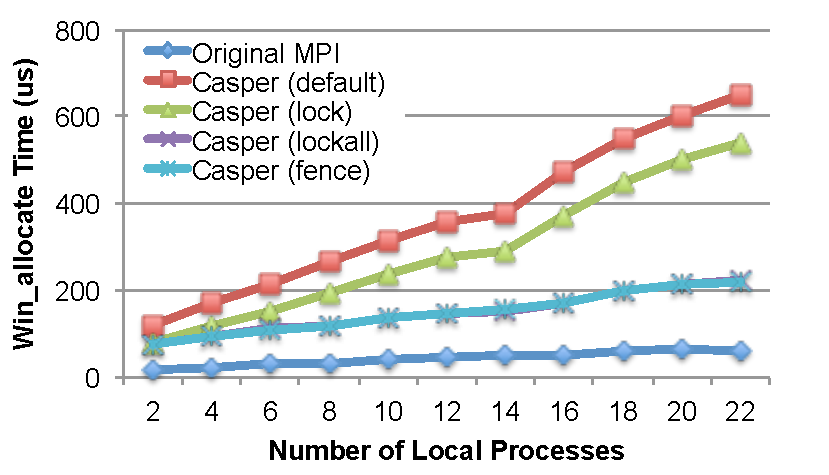
\includegraphics[width=0.85\columnwidth]{figures/casper/eva_edison_overhead_win_alloc.pdf}
  \label{fig:eva-cray-overh-win-alloc}
}
\subfigure[Fence and PSCW overhead]{
  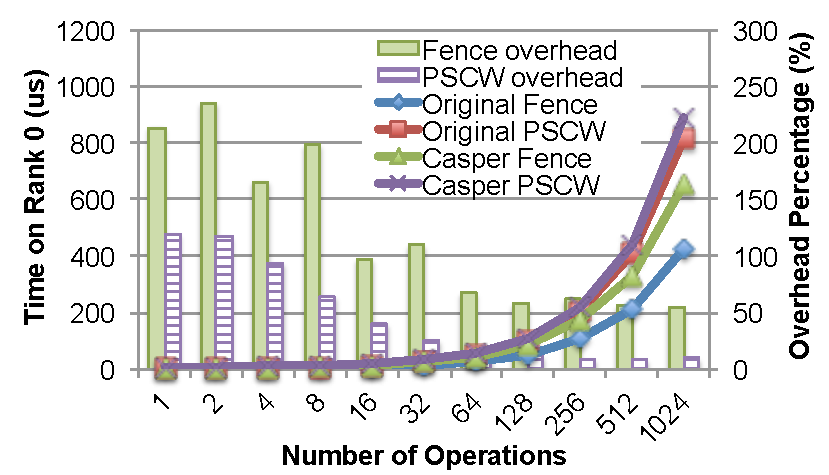
\includegraphics[width=0.85\columnwidth]{figures/casper/eva_edison_overhead_fence_pscw.pdf}
  \label{fig:eva-cray-overh-active}
}
% \subfigure[RMA operation segmentation]{
%   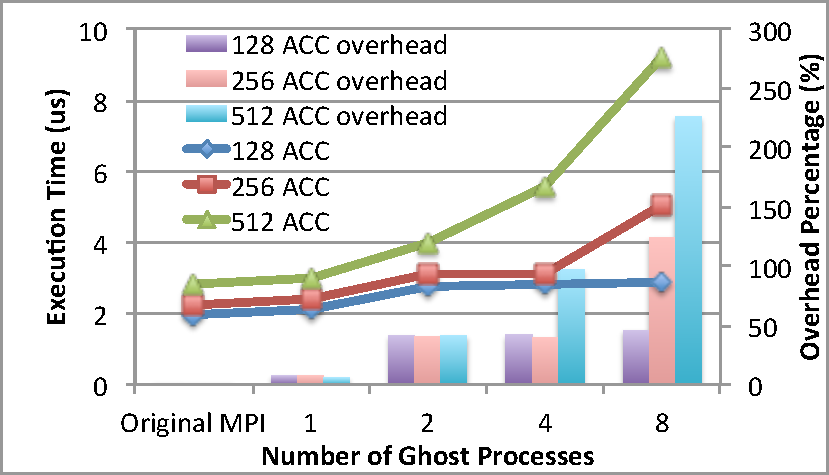
\includegraphics[width=0.62\columnwidth]{figures/casper/eva_cray_overhead_op_seg.pdf}
%   \label{fig:eva-cray-overh-op-seg}
% }
% \subfigure[Overhead when locking process itself on InfiniBand using MPICH-MXM.]{
%   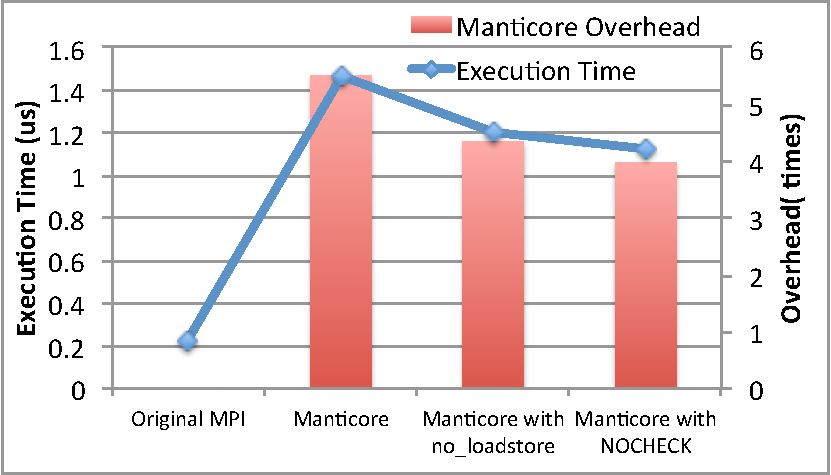
\includegraphics[width=0.63\columnwidth]{figures/casper/eva_mxm_overhead_lockself.pdf}
%   \label{fig:eva-mxm-overh-lockself}
% }
% \subfigure[Overhead of SHM RMA operation redirection on InfiniBand using MPICH-MXM.]{
%   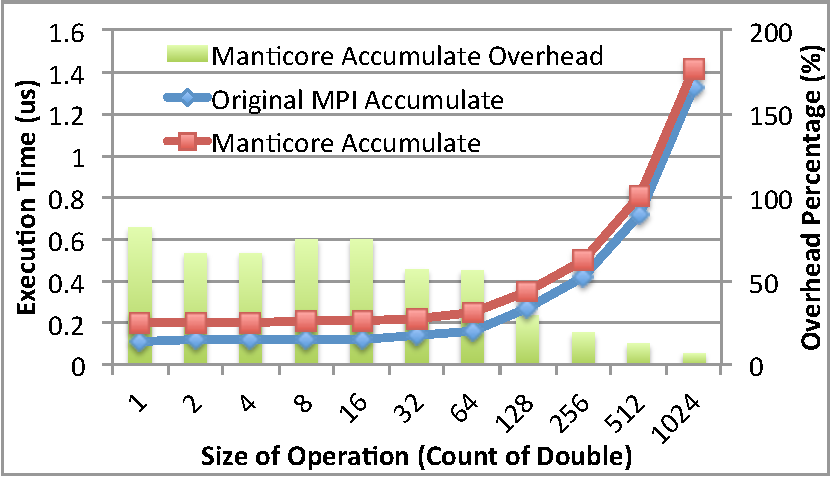
\includegraphics[width=0.63\columnwidth]{figures/casper/eva_mxm_overhead_op_shm.pdf}
%   \label{fig:eva-mxm-overh-op-shm}
% }
% \subfigure[Overhead of Inter-node RMA operation redirection]{
%   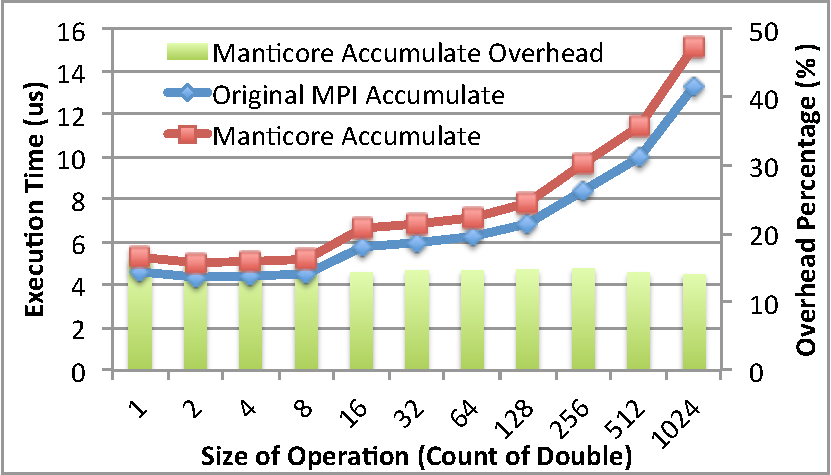
\includegraphics[width=0.63\columnwidth]{figures/casper/eva_mxm_overhead_op_inter.pdf}
%   \label{fig:eva-mxm-overh-op-inter}
% }
% \subfigure[Overhead of RMA operation segmentation]{
%   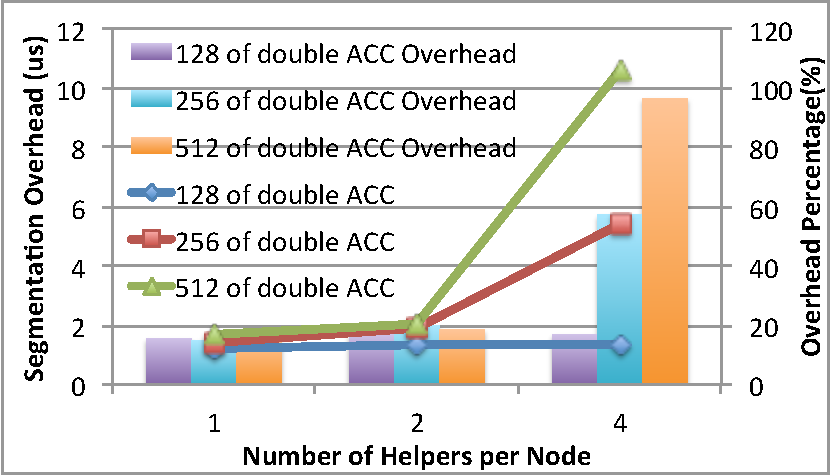
\includegraphics[width=0.63\columnwidth]{figures/casper/eva_mxm_overhead_op_seg.pdf}
%   \label{fig:eva-mxm-overh-op-seg}
% }
% \caption{Overhead Analysis on InfiniBand cluster using MPICH.}
% \footnotesize{\textcolor{red}{Why internode op overhead increase ? }}
% \label{fig:eva-mxm-overh}
% \end{figure*}
% \begin{figure*}
% \centering
% \subfigure[Lockall overhead on Cray X30.]{
%   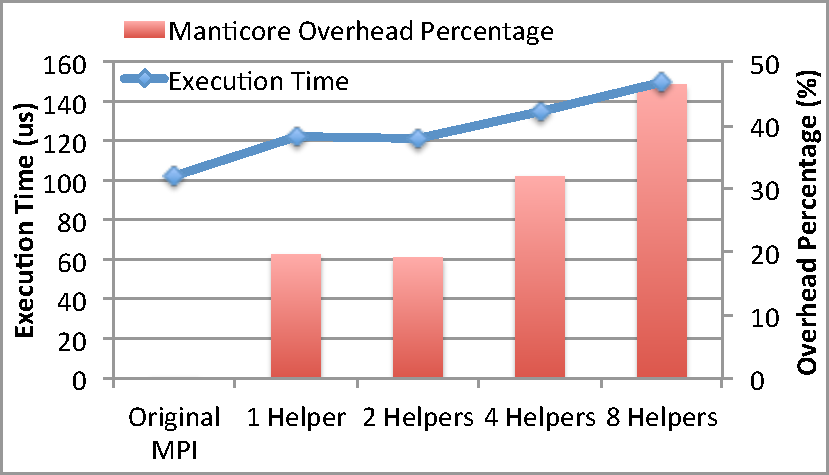
\includegraphics[width=0.63\columnwidth]{figures/casper/eva_cray_overhead_lockall.pdf}
%   \label{fig:eva-cray-overh-lockall}
% }
% \subfigure[Local lock]{
%   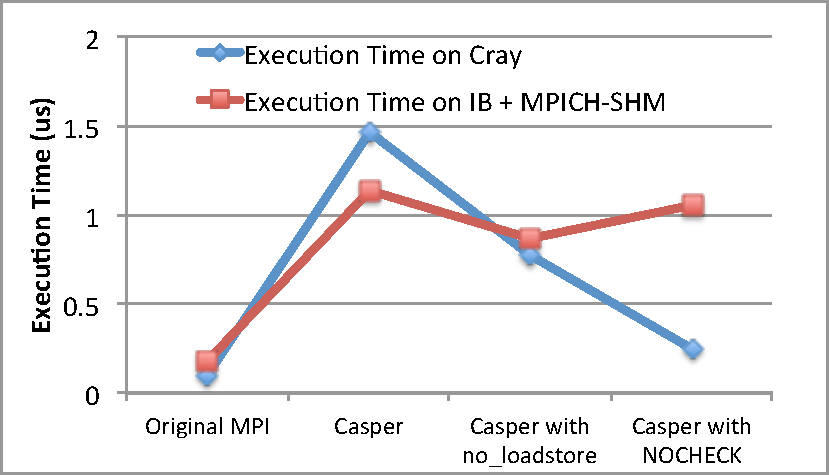
\includegraphics[width=0.63\columnwidth]{figures/casper/eva_overhead_lockself.pdf}
%   \label{fig:eva-overh-lockself}
% }
% \subfigure[Overhead of SHM RMA operation redirection on Cray X30.]{
%   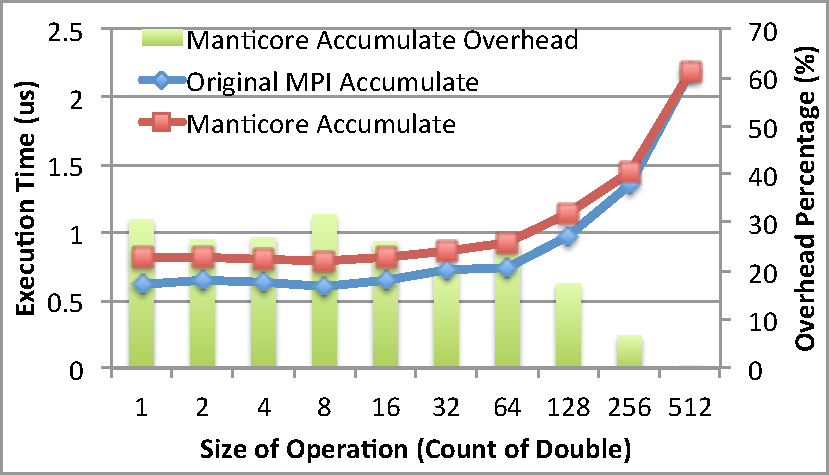
\includegraphics[width=0.63\columnwidth]{figures/casper/eva_cray_overhead_op_shm.pdf}
%   \label{fig:eva-cray-overh-op-shm}
% }
% \subfigure[Overhead of Inter-node RMA operation redirection]{
%   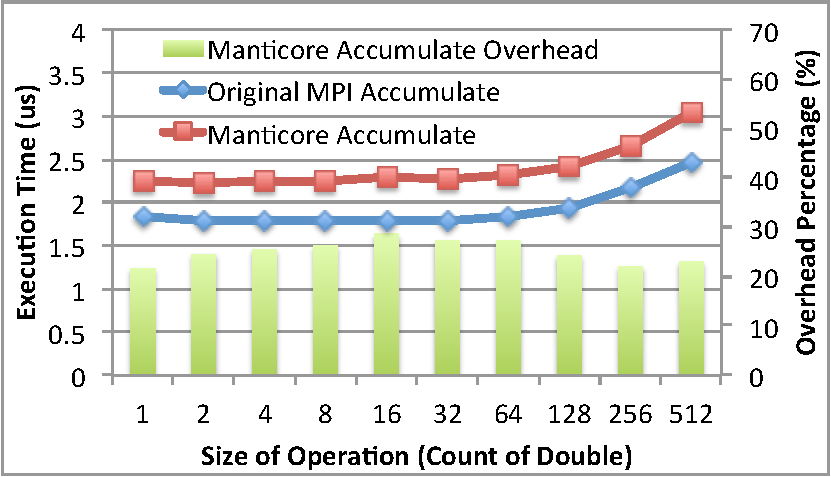
\includegraphics[width=0.63\columnwidth]{figures/casper/eva_cray_overhead_op_inter.pdf}
%   \label{fig:eva-cray-overh-op-inter}
% }
% \vspace{-1.5ex}
\caption{Overhead analysis.}
\label{fig:eva-cray-overh}
% \vspace{-4.0ex}
\end{figure}


%%%%%%%%%%%%%%%%%%%%%%%%%%%%%%%%%%%%%%%%%%%%%%%%%%%%
\subsection{Asynchronous Progress }\label{sec:eva-scala}
%%%%%%%%%%%%%%%%%%%%%%%%%%%%%%%%%%%%%%%%%%%%%%%%%%%%

In the section, we demonstrate the asynchronous progress improvements
achieved in various scenarios.

%%%%%%%%%%%%%%%%%%%%%%%%%%%%%%%%%%%%%%%%%%%%%%%%%%%%
\subsubsection{Different Synchronization Modes}\label{sec:eva-overlap}
%%%%%%%%%%%%%%%%%%%%%%%%%%%%%%%%%%%%%%%%%%%%%%%%%%%%

Our first experiment demonstrates the improvement of computation and
communication overlap in passive and active-target modes using Casper.
Two interconnected processes are used in each mode.  In
the passive-target mode, one process issues
\emph{lockall--accumulate--unlockall} to another process while that
process is blocking in computation.
Figure~\ref{fig:eva-cray-async-lockall} shows the results on
the Cray XC30.  As expected, with the original MPI the execution time
on the origin increases with wait time on the target, which means that the
origin is blocked by the computation on the target.  All asynchronous
progress approaches relieve this issue.  We note, however, that both
the DMAPP and thread approaches have more overhead than Casper does.

The overhead with using the MPICH asynchronous thread comes from the expensive
thread-multiple safety and lock contention.  DMAPP-based asynchronous
progress, however, does not involve thread-multiple safety and also
wakes up background threads only when a message arrives.  Therefore, to
analyze the reason for this overhead, we performed a test in which one
process does \emph{lockall--accumulate--unlockall} and the other
process does a \textit{dgemm} computation.  As shown in
Figure~\ref{fig:eva-cray-dmapp-overhead}, when we increase the number
of ACCUMULATEs issued in each iteration, DMAPP's overhead also
increases.  To further analyze this situation, we measured the number of system
interrupts. We found that they increased with the number of
ACCUMULATEs as well and were clearly becoming a bottleneck with
increasing numbers of operations.

% \begin{figure}[h]
% \begin{CenteredBox}
% \begin{lstlisting}[linewidth=0.73\columnwidth]
% MPI_Win_lock_all(win);
% if (rank == 0){
%     MPI_Accumulate(...);
%     MPI_Win_flush(1, win);
% }else{
%     while(MPI_Wtime() - start < WAIT_TIME);
%     MPI_Test(...);
% }
% MPI_Win_unlock_all(win);
% \end{lstlisting}
% \end{CenteredBox}
% \caption{Overlap improvement microbenchmark.}
% \label{code:test-src}
% \end{figure}

In the active-target mode, since both fence and PSCW require internal
synchronization in Casper, the origin has to wait for the completion
of the epoch on the target.  Thus, in an experiment similar to that for
the passive mode, we measured the time for
\emph{fence--accumulate--fence} on one process while another process
performs \emph{fence--100~$\mu$s busy waiting--fence} as shown in
Figure\ref{fig:eva-cray-async-fence}.  We notice that when a small
number of operations are issued during fence, asynchronous progress is
beneficial.  But when the communication takes more time than the delay
on the target, which is the maximum time Casper can overlap (larger
than 128 in the figure), the percentage improvement decreases, as
expected.  PSCW follows a similar trend. Both DMAPP and
thread asynchronous progress show significant overhead compared with that of the original
MPI execution.

\begin{figure*}
\centering
\subfigure[Passive-target RMA]{
  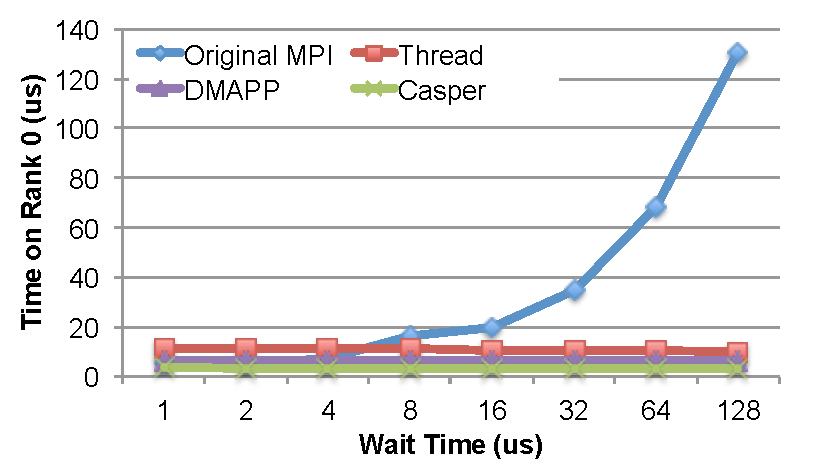
\includegraphics[width=0.64\columnwidth]{figures/casper/eva_cray_test2pe_s.pdf}
  \label{fig:eva-cray-async-lockall}
}
\subfigure[Fence RMA]{
  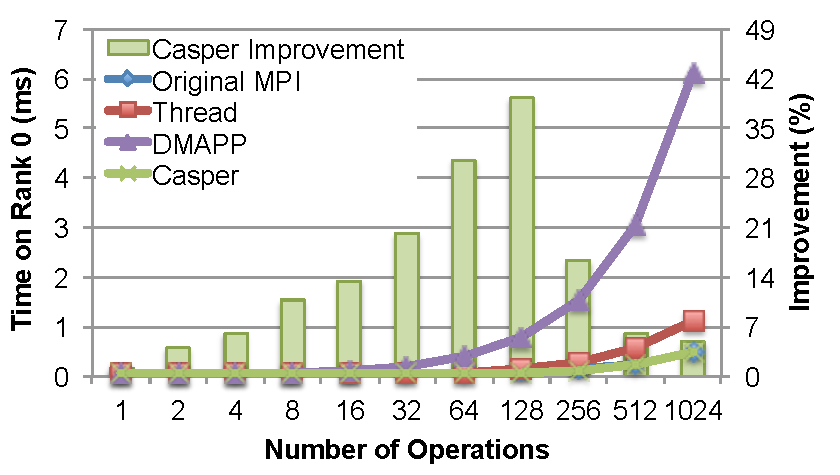
\includegraphics[width=0.64\columnwidth]{figures/casper/eva_cray_async_fence.pdf}
  \label{fig:eva-cray-async-fence}
}
\subfigure[Overhead of DMAPP interrupts]{
  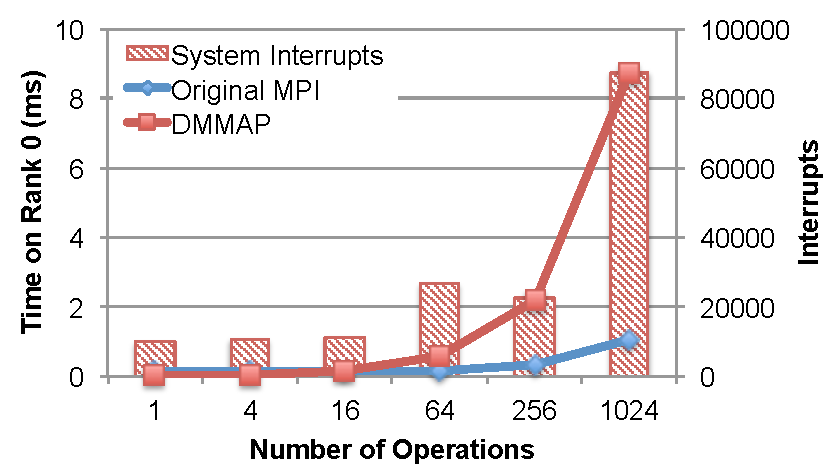
\includegraphics[width=0.64\columnwidth]{figures/casper/eva_cray_dmapp_overhead.pdf}
  \label{fig:eva-cray-dmapp-overhead}
}
% \subfigure[PSCW RMA\textcolor{blue}{[TODO]}]{
%   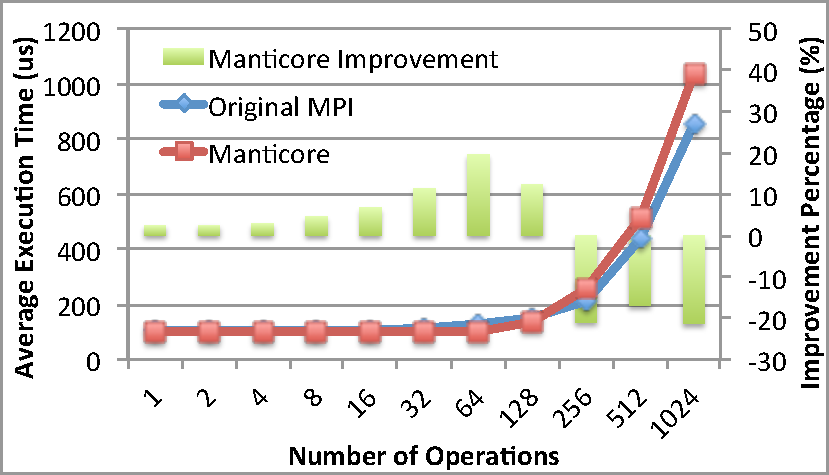
\includegraphics[width=0.63\columnwidth]{figures/casper/eva_cray_async_pscw.pdf}
%   \label{fig:eva-cray-async-pscw}
% }
% \vspace{-1.0ex}
\caption{Overlap improvement using two interconnected processes on
Cray XC30.}
\label{fig:eva-comm-overlap}
% \vspace{-4.0ex}
\end{figure*}


% \begin{figure}[h]
% \centering
% 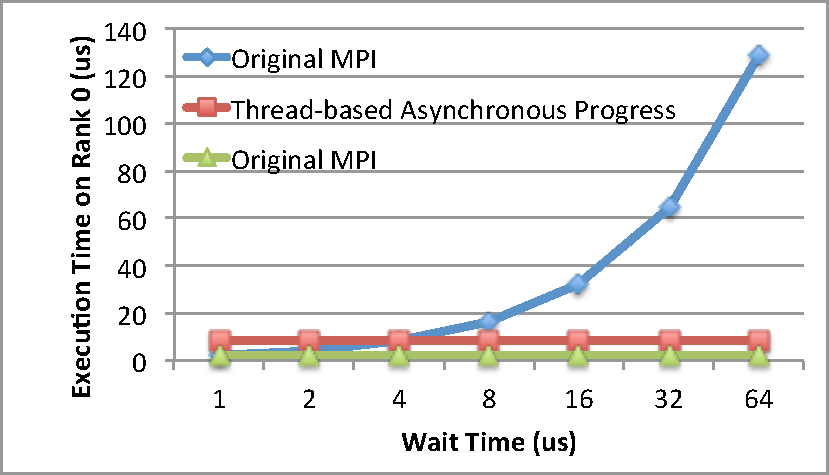
\includegraphics[width=0.8\columnwidth]{figures/casper/eva_fusion_lockall_shm_np2.pdf}
% \caption{Lockall asynchronism improvement using two processes on
% a shared memory node using MPICH-SHM.}
% \end{figure}

%%%%%%%%%%%%%%%%%%%%%%%%%%%%%%%%%%%%%%%%%%%%%%%%%%%%
\subsubsection{Different RMA implementations}\label{sec:eva-rma}
%%%%%%%%%%%%%%%%%%%%%%%%%%%%%%%%%%%%%%%%%%%%%%%%%%%%

The second experiment focuses on the scalability of asynchronous
progress with different RMA implementations.  In this experiment every
process communicates with all the other processes in a
\emph{communication--computation--communication} pattern.  We use one
RMA operation (size of a double) in the first communication,
100~$\mu$s of computation, and ten RMA operations (each size double)
in the second communication.

On Cray XC30, we use one process per node and scale the number of
nodes for both ACCUMULATE and PUT, as shown in
Figures~\ref{fig:eva-scala-cray-acc} and
\ref{fig:eva-inter-np-1core-put}.  We note that DMAPP enables direct
RMA for PUT\slash GET with basic datatypes in Cray MPI, but it involves
interrupts for ACCUMULATE operations.  Consequently, Casper
outperforms the other approaches for ACCUMULATE, while achieving the
same performance as that of DMAPP for PUT\slash GET.  The thread
asynchronous progress is always expensive and even worse than that of the
original MPI when a large number of processes are communicating.

On the Fusion cluster, we compared Casper with MVAPICH by also using
one process per node. Figure~\ref{fig:eva-fusion-acc} indicates that Casper improves
asynchronous progress for ACCUMULATE, which is still implemented with
software active messages in MVAPICH.  The thread asynchronous progress
again shows significant overhead.  We also measured the performance of
PUT\slash GET operations; as expected, the performance
of Casper was identical to that of original MPI since these operations
are implemented directly in hardware.  The performance numbers are not
shown here because of space limitations.


\begin{figure*}
\centering
\subfigure[Accumulate on Cray XC30.]{
  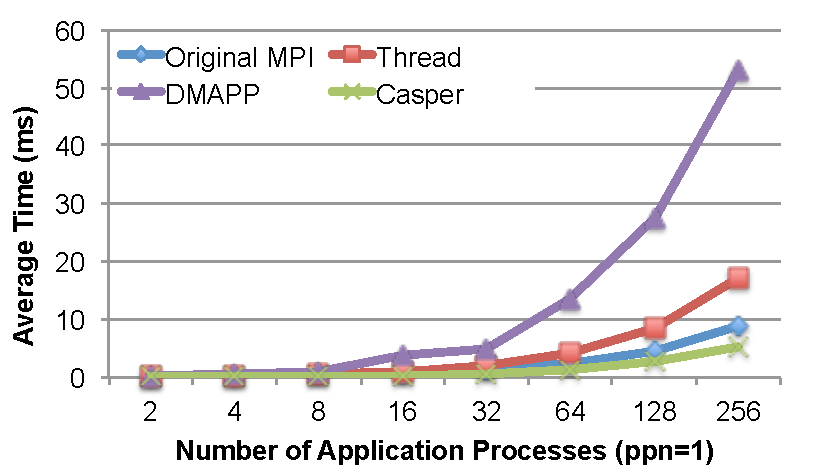
\includegraphics[width=0.64\columnwidth]{figures/casper/eva_cray_inter_np_1core.pdf}
  \label{fig:eva-scala-cray-acc}
}
\subfigure[Put on Cray XC30.]{
  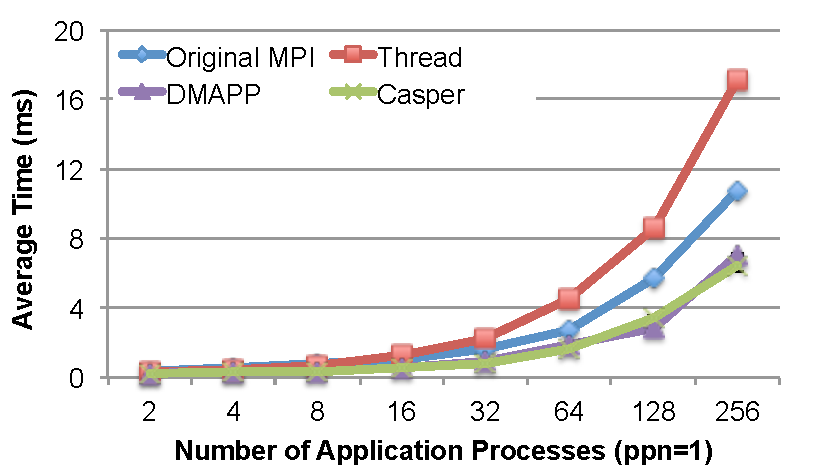
\includegraphics[width=0.64\columnwidth]{figures/casper/eva_cray_inter_np_1core_put.pdf}
  \label{fig:eva-inter-np-1core-put}
}
\subfigure[Accumulate on Fusion using MVAPICH.]{
  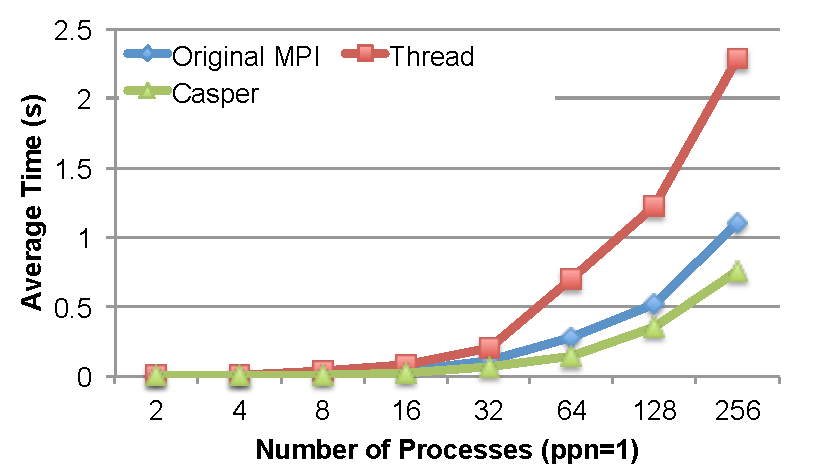
\includegraphics[width=0.64\columnwidth]{figures/casper/eva_fusion_inter_np_1core.pdf}
  \label{fig:eva-fusion-acc}
}
% \subfigure[Put on IB cluster using MVAPICH.]{
%   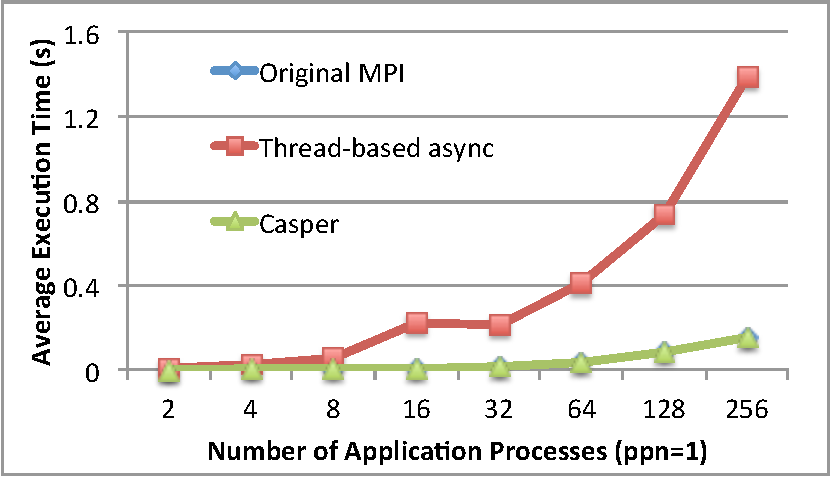
\includegraphics[width=0.48\columnwidth]{figures/casper/eva_fusion_inter_np_1core_put.pdf}
%   \label{fig:eva-fusion-put}
% }
% \subfigure[Accumulate in shared memory using MPICH.]{
%   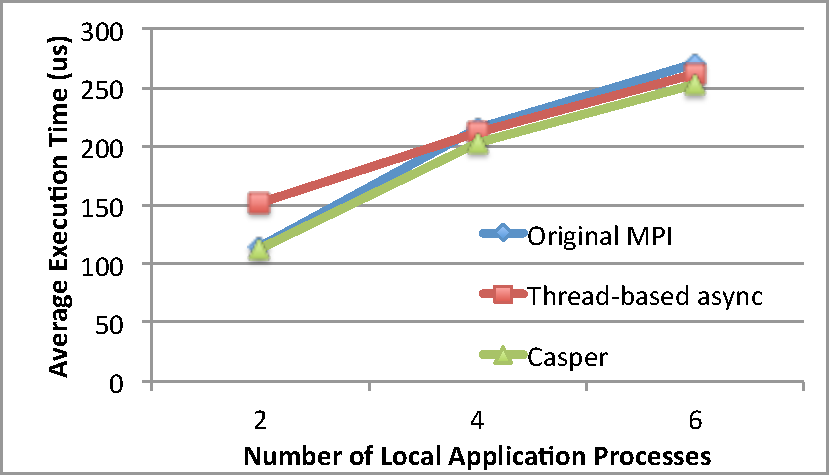
\includegraphics[width=0.62\columnwidth]{figures/casper/eva_mxm_async_acc.pdf}
%   \label{fig:eva-mxm-acc}
% }
% \subfigure[Lockall in shared memory using MPICH.]{
%   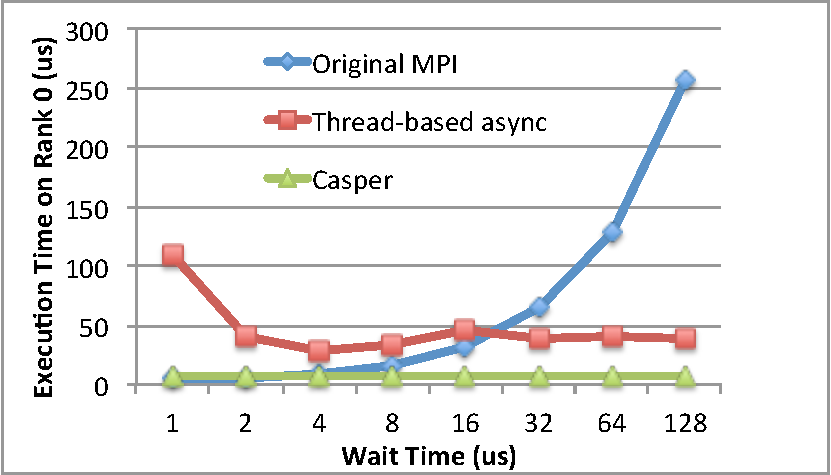
\includegraphics[width=0.62\columnwidth]{figures/casper/eva_mxm_async_lockall.pdf}
%   \label{fig:eva-mxm-lock}
% }
% \vspace{-1.0ex}
\caption{Asynchronous progress on different platforms.}
\label{fig:eva-scala}
% \vspace{-1.0ex}
\end{figure*}

% We also compared Casper with MPICH-SHM which supports direct RMA for
% all operations on shared memory.  Figure~\ref{fig:eva-mxm-acc} shows
% the performance of ACCUMULATE in the same
% \emph{communication--computation--communication} experiment described
% above.  It shows that Casper does not effect the performance of direct
% RMA operations on shared memory either.  However, although RMA
% operations are performed as direct RMA on shared memory,
% passive-target synchronization calls, such as \emph{lockall}, may
% internally involve two-sided communication which requires remote
% process to poll MPI progress.  We evaluate the asynchronous progress
% of \emph{lockall} on shared memory by measuring a test in which rank 0
% performs \emph{lockall--one accumulate--unlockall} to all the other
% local processes, and the others are busy computing.
% Figure~\ref{fig:eva-mxm-lock} shows the results using 6 processes on a
% single node.  As expected, with increasing computation on the target,
% the origin takes an increasing amount of time to finish its
% communication with original MPI.  Although both the asynchronous
% thread and Casper resolve this issue, the thread approach shows more
% overhead when the number of idle cores is not sufficient for running
% these per-process threads and results in core oversubscription (we run
% 6 processes on a 8 cores node).  Moreover, we notice that the thread
% asynchronous threads produce more overhead when the main thread of the
% waiting process only waits for 1 or 2~$\mu$s before entering into MPI
% stack and hence results in frequent lock contention.


%%%%%%%%%%%%%%%%%%%%%%%%%%%%%%%%%%%%%%%%%%%%%%%%%%%%
\subsection{Performance Optimization}\label{sec:eva-load}
%%%%%%%%%%%%%%%%%%%%%%%%%%%%%%%%%%%%%%%%%%%%%%%%%%%%

Our third set of microbenchmarks focuses on the different load-balancing
optimizations discussed in Section~\ref{sec:multi-ghost}.

%%%%%%%%%%%%%%%%%%%%%%%%%%%%%%%%%%%%%%%%%%%%%%%%%%%%
\subsubsection{Static Rank Binding}\label{sec:eva-static-rank}
%%%%%%%%%%%%%%%%%%%%%%%%%%%%%%%%%%%%%%%%%%%%%%%%%%%%

Figure~\ref{fig:eva-sta-load} shows our measurements with static rank
binding on Cray X30.  In the first experiment
(Figure~\ref{fig:eva-cray-sta-load-rank-nnp}) we show the static rank
binding with increasing number of processes when each process sends one
accumulate message (size of double) to every other process in the
system.  We use 16 processes per node and evaluate Casper with up to 8
ghost processes on each node.
Our results indicate that two ghost processes are sufficient
when up to 32 processes communicate; when more processes
communicate, however, configurations with larger numbers of ghost processes tend
to perform better.
The reason is that the number of
incoming RMA operations increases with more processes, thus requiring
more ghost processes computing to keep up.

Figure~\ref{fig:eva-cray-sta-load-rank-nop} shows a similar
experiment but increases the number of accumulate operations while
keeping the user process count constant at 32 (2 nodes with 16
processes each).  The results show a trend similar to that of the previous
experiment, with more ghost processes benefiting when the number of
operations per process is larger than 8.

%%%%%%%%%%%%%%%%%%%%%%%%%%%%%%%%%%%%%%%%%%%%%%%%%%%%
\subsubsection{Static Segment Binding}\label{sec:eva-static-seg}
%%%%%%%%%%%%%%%%%%%%%%%%%%%%%%%%%%%%%%%%%%%%%%%%%%%%

In this experiment we evaluate the performance of the static segment binding approach.  Such an approach is expected to be especially
beneficial when the application allocates uneven-sized windows and
receives a large number of operations that need to be processed in
software.  Figure~\ref{fig:eva-cray-sta-load-seg} demonstrates this
pattern.  We used 16 nodes with 16 processes and up to 8 ghost
processes per node.  The first
process of every node allocates a 4-kilobyte window (512 count of
double), while the others only allocate 16~bytes.  Then each process
performs a \emph{lockall--accumulate--unlockall} pattern on all the
other processes.  We increase the number of ACCUMULATEs to each
process whose local rank is 0 while issuing a single operation to
other processes.  As shown in the figure, performance improves with
increasing numbers of ghosts, because the large window is divided into
more segments and the communication issued to different segments is
handled by different ghosts.

\begin{figure*}
\centering
\subfigure[Static Rank Binding: Increasing Processes.]{
  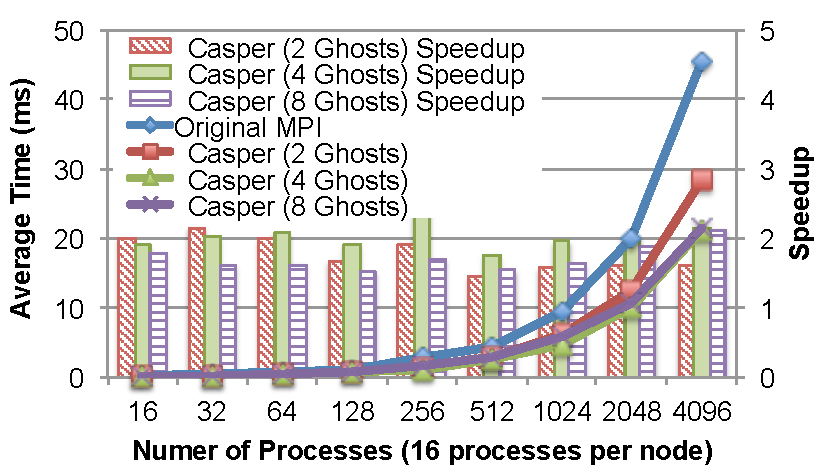
\includegraphics[width=0.64\columnwidth]{figures/casper/eva_cray_static_load_nnp.pdf}
  \label{fig:eva-cray-sta-load-rank-nnp}
}
\subfigure[Static Rank Binding: Increasing operations.]{
  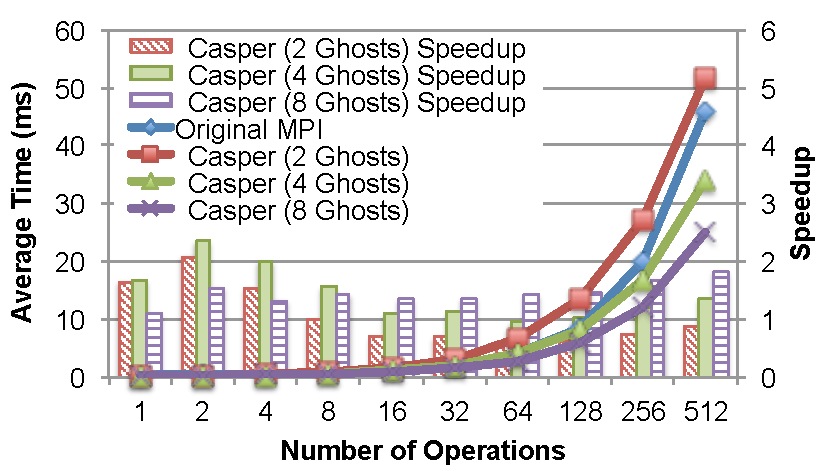
\includegraphics[width=0.64\columnwidth]{figures/casper/eva_cray_static_load_nop.pdf}
  \label{fig:eva-cray-sta-load-rank-nop}
}
\subfigure[Static Segment Binding: Uneven Window Size]{
  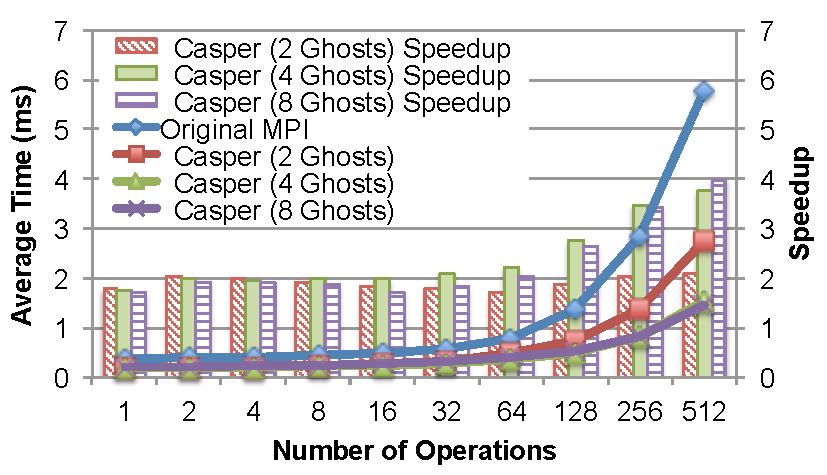
\includegraphics[width=0.64\columnwidth]{figures/casper/eva_cray_static_load_nseg.pdf}
  \label{fig:eva-cray-sta-load-seg}
}
% \vspace{-1.0ex}
\caption{Load balancing in static binding on Cray XC30.}
\label{fig:eva-sta-load}
% \vspace{-2.0ex}
\end{figure*}


%%%%%%%%%%%%%%%%%%%%%%%%%%%%%%%%%%%%%%%%%%%%%%%%%%%%
\subsubsection{Dynamic Binding}\label{sec:eva-dynamic-bind}
%%%%%%%%%%%%%%%%%%%%%%%%%%%%%%%%%%%%%%%%%%%%%%%%%%%%

To test our dynamic binding
approaches, we designed three microbenchmarks, all of which are
executed on 16 nodes with 20 user processes and 4 ghost processes per
node.

Figure~\ref{fig:eva-cray-runtime-load-random} shows the results of an experiment
in which all processes perform a \emph{lockall--put--unlockall} pattern
to all the other processes, but only the first rank of each node
receives an increasing number of PUT operations (varied on the x-axis
of the graph), while the others receive only one PUT operation.  Our
random load balancing simply chooses the ghost processes in the order
of its local rank for each target process.  Thus, all the PUT
operations are always equally distributed to the ghosts on each node
achieving much better performance that with static binding.

Figure~\ref{fig:eva-cray-runtime-load-op} uses a variant of the
previous experiment in which each process performs an uneven
\emph{lockall--accumulate--put--unlockall} pattern to all other
processes. In this case, random load balancing arbitrarily picks the
ghost process for each PUT operation but sends all ACCUMULATE
operations to the same ghost process (in order to maintain ordering
and atomicity guarantees).  Thus, the ghost process that is handling
both ACCUMULATE and PUT operations would end up having to handle more
operations than would the other ghost processes.  Our
``operation-counting'' approach, on the other hand, keeps track of
which ghost process has been issued how many operations and balances
the operations appropriately, thus allowing it to achieve better
performance than the random approach does.

Our third experiment,
uses yet another variant of the previous experiments by varying the
size of the operations while keeping the number of operations
constant.  Each process performs a
\emph{lockall--accumulate--put--unlockall} pattern, but only the
processes whose local rank is 0 receive increasing sizes of PUTs and
ACCUMULATEs (varied on the x-axis), while the others receive only one
double PUT and accumulate.
Figure~\ref{fig:eva-cray-runtime-load-byte} shows the results.
As expected, neither random nor
operation-counting algorithms can handle this case well, although
our ``byte-counting'' approach outperforms both of them.

\begin{figure*}
\centering
\subfigure[Random: Uneven Number of Put.]{
  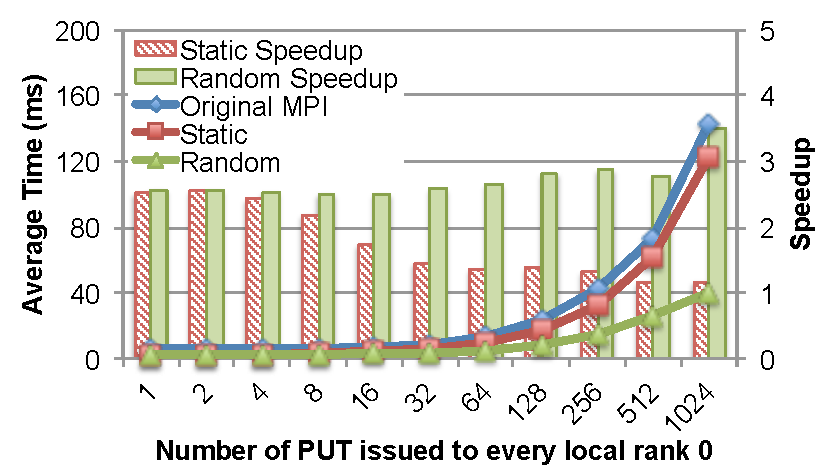
\includegraphics[width=0.64\columnwidth]{figures/casper/eva_cray_runtime_load_random.pdf}
  \label{fig:eva-cray-runtime-load-random}
}
\subfigure[OP-counting: Uneven Number of Put/ACC.]{
  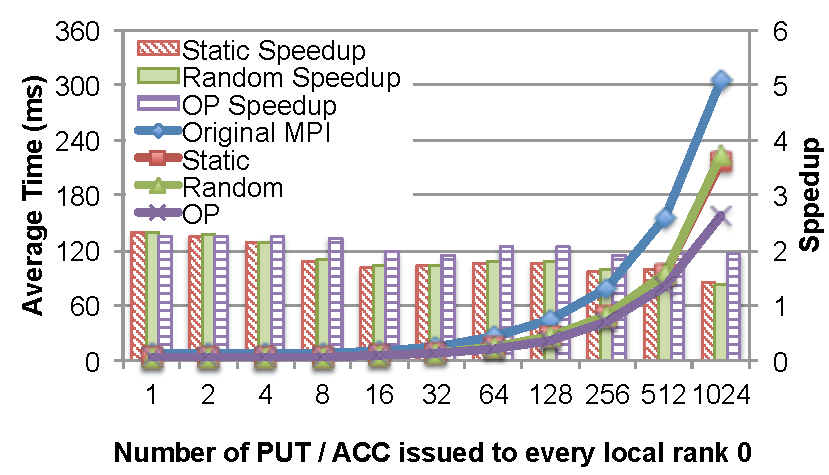
\includegraphics[width=0.64\columnwidth]{figures/casper/eva_cray_runtime_load_op.pdf}
  \label{fig:eva-cray-runtime-load-op}
}
\subfigure[Byte-counting: Uneven Size of Put/ACC.]{
  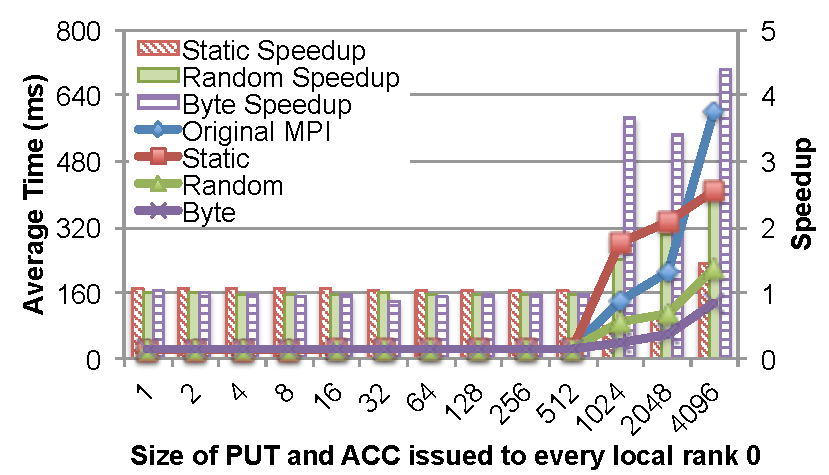
\includegraphics[width=0.64\columnwidth]{figures/casper/eva_cray_runtime_load_byte.pdf}
  \label{fig:eva-cray-runtime-load-byte}
}
% \vspace{-1.0ex}
\caption{Dynamic load balancing on Cray XC30.}
\label{fig:eva-runtime-load}
% \vspace{-4.0ex}
\end{figure*}

% %%%%%%%%%%%%%%%%%%%%%%%%%%%%%%%%%%%%%%%%%%%%%%%%%%%%
% \subsubsection{Memory Locality Comparison}\label{sec:eva-locality}
% %%%%%%%%%%%%%%%%%%%%%%%%%%%%%%%%%%%%%%%%%%%%%%%%%%%%
% The last microbenchmark measures the overhead when
% ghost process is located in a different NUMA domain with
% the application process. We simply use two interconnected processes
% each with a ghost process on its node, one process issues
% \emph{lock-100 accumulate-unlock} to the second process while
% the second one waits in MPI barrier. Figure~\ref{fig:eva-cray-locality}
% shows that significant overhead occurs on Cray XC30 when the ghost
% process is located in a different NUMA domain and accesses the
% memory of application process across domain. The overhead
% even increases with increasing size of operations, 120\% overhead
% is produced when issuing 512 could of double(4097~Bytes) operation .

% \begin{figure}[h]
% \centering
% 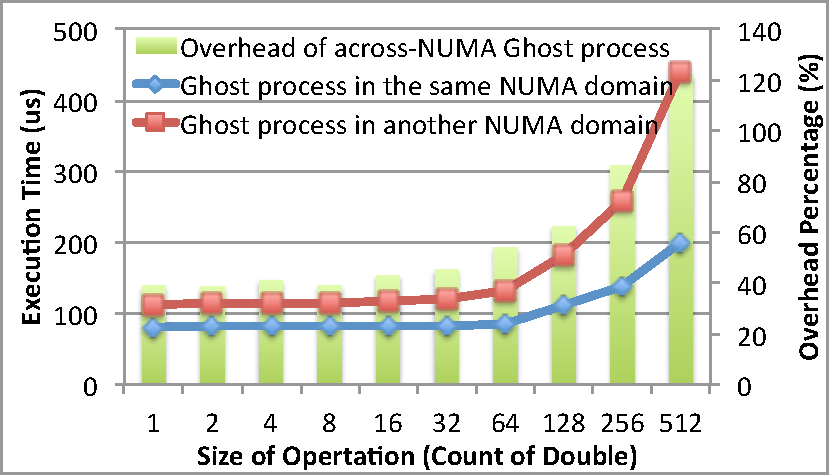
\includegraphics[width=0.8\columnwidth]{figures/casper/eva_edison_locality.pdf}
% \caption{Comparison of two cases with different ghost process location.}
% \label{fig:eva-cray-locality}
% \end{figure}




%%%%%%%%%%%%%%%%%%%%%%%%%%%%%%%%%%%%%%%%%%%%%%%%%%%%
\subsection{NWChem Quantum Chemistry Application}\label{sec:eva-realapp}
%%%%%%%%%%%%%%%%%%%%%%%%%%%%%%%%%%%%%%%%%%%%%%%%%%%%

NWChem~\cite{NWChem63} is a computational chemistry application suite
offering many simulation capabilities.  For massively
parallel simulations, a common method employed is coupled-cluster
theory (CC), for which NWChem has extensive
functionality~\cite{Hirata:2003:JPCA:TCE} and excellent
performance~\cite{Apra:2009:SC:NWChem}.  For data movement, NWChem uses the Global
Arrays~\cite{GA_SC94} toolkit, which has been
implemented on a number of platforms natively and as a portable
implementation over MPI RMA~\cite{dinan12:armci_mpi}.

Because CC simulations are one of the most common usages of NWChem in
the context of large clusters or supercomputers, our experiments focus
on the most popular CC method, CCSD(T).
Two molecules are considered: the water cluster (H$_2$O)$_n$
($n=16$)---denoted W$n$ for short---and C$_{20}$, obtained
from the NWChem QA test suite (\texttt{QA/tests/tce\_c20\_triplet}).
For the water cluster, we used double-zeta basis sets (cc-pVDZ from
the NWChem basis set library), which are reasonable for this class of
problems.  We compared Casper with both the original MPI and two
thread-based approaches.
The first approach employs oversubscribed cores
(Thread~(O)), where every thread and its MPI process execute on
the same core; the second approach uses dedicated cores (Thread~(D)),
where threads and MPI processes are on separate cores. We used the same total
number of cores in all approaches, some of which are dedicated to
asynchronous ghost processes\slash threads as listed in Table~\ref{tab:eva-nwcore}.

\begin{table}\scriptsize
\begin{center}
\caption{Core deployment in NWChem evaluation on Cray XC30.}\label{tab:eva-nwcore}
\begin{tabular}{|c|c|c|}
\hline
& Computing Cores & Async Cores \\
\hline
Original MPI & 24 & 0 \\
Casper & 20 & 4 \\
Thread (O) & 24 & 24 \\
Thread (D) & 12 & 12 \\
\hline
\end{tabular}
\end{center}
% \vspace{-4.0ex}
\end{table}

Figures~\ref{fig:eva-edison-nw-w16} and
\ref{fig:eva-edison-nw-c20-ccsd} report timings for a single
iteration of CCSD, which is a communication-intensive solver composed
of more than a dozen tensor contractions of varying size.  For smaller
problems, when computation dominates, asynchronous progress is more
important because the application is calling MPI relatively
infrequently.  At larger scale, the computation time decreases, and the
communication is more frequent; hence the improvement with Casper is
less.  The (T) portion of the CCSD(T) methods is much more
compute-intensive. Hence, the time between MPI calls can be
large, and thus the impact of asynchronous progress is
significant.  Each process fetches remote data, then does significant
computation---over and over. As a result, the lack of progress causes
processes to stall, waiting on GET operations to be satisfied remotely.
Figure~\ref{fig:eva-edison-nw-c20-ccsdt} shows the significance of
asynchronous progress at all scales.  Relative to the original
version, Casper is almost twice as fast; but thread-based asynchronous
progress is far less effective. The reason is that although both approaches
improve asynchronous progress in communication, the thread-based
solutions significantly degrade the performance of computation, either by
core oversubscription or by appropriation of half of the computing cores.

\begin{figure*}
\centering
\subfigure[CCSD for W16=(H$_2$O)$_{16}$ with pVDZ]{
  \includegraphics[width=0.64\columnwidth]{figures/casper/eva_edison_nwchem_w16_dz.pdf}
  \label{fig:eva-edison-nw-w16}
}
\subfigure[CCSD for C$_{20}$ with pVTZ]{
  \includegraphics[width=0.64\columnwidth]{figures/casper/eva_edison_nwchem_tce_c20_ccsd.pdf}
  \label{fig:eva-edison-nw-c20-ccsd}
}
\subfigure[(T) portion of CCSD(T) for C$_{20}$ with pVTZ]{
  \includegraphics[width=0.64\columnwidth]{figures/casper/eva_edison_nwchem_tce_c20_ccsdt.pdf}
  \label{fig:eva-edison-nw-c20-ccsdt}
}
% \vspace{-1.0ex}
\caption{NWChem TCE coupled cluster methods on Cray XC30.}
\label{fig:eva-nwchem}
% \vspace{-4.0ex}
\end{figure*}



\chapter{Adaptable Asynchronous Progress}\label{chp:adpt}

% \section{Introduction}
% \label{sec:intro}
In our previous work~\cite{casper}, we proposed ``Casper,''
a process-based asynchronous progress solution for MPI on multi- and
many-core architectures. An alternative to traditional thread- and
interrupt-based models, Casper provides a distinct set of benefits
for applications, which we believe are more appropriate for large
many-core architectures. The philosophy of the Casper architecture
is centered on the notion that since the number of cores in the system
is growing rapidly, there can be always a few idle cores during the
execution, thus dedicating them for helping with asynchronous progress
might be better than using an interrupt-based model. Similarly, the use
of processes rather than threads allows Casper to control the amount
of sharing, thus reducing thread-safety overheads associated with
multithreaded models, as well as to control the number of cores being
utilized for asynchronous progress.

The central idea of Casper is the ability of processes to share
memory by mapping a common memory object into their address spaces
by using the MPI-3 shared memory windows interface.  Specifically, Casper
keeps aside a small user-specified number of cores on a multi- or
many-core environment as ``ghost processes.''  When the application
process tries to allocate a remotely accessible memory window, Casper
intercepts the call and maps such memory into the ghost processes'
address space.  Casper then intercepts all RMA operations to the user
processes on this window and redirects them to the ghost processes
instead.

We have evaluated Casper by using various micro-benchmarks and a real
quantum chemistry application, NWChem, and shown significant performance
improvement in our previous work. However, the performance is still not
ideal. Although we have achieved signification improvement in some
computation-intensive phase such as the time-consuming (T) portion in
the ``gold standard'' CCSD(T) simulation~\cite{casper}\cite{casper-scaling},
we also observe performance degradation in some communication-intensive
phases such as CCSD iteration. This is because, in communication-intensive
phases, the asynchronous progress may not be necessary since the target
processes can frequently make MPI calls and thus handle the operations
issued to them as targets by themselves. Furthermore, when the amount of RMA
operations becomes large, the operation redirection in Casper can even
result in over workload issue. That is, a large amount of operations
were originally issued to different user target processes, but are
redirected to a few ghost processes in Casper. Such situation can result in
communication performance degradation if the performance benefit from
asynchronous progress is less than the performance loss in the operation
overloading on ghost processes.

In this paper, we propose an adaptation mechanism for Casper, providing
the capability to dynamically adapt the asynchronous progress
for multiple execution phases performing varying communication characteristics.
The adaptation approach allows application to dynamically redirect all
RMA communication to the ghost processes for computation-intensive phase
that requiring efficient asynchronous progress, with avoiding inefficient
redirection for communication-intensive phase.
We note that, the cores dedicated to background ghost processes are always
kept aside from the application even when the asynchronous progress is disabled.

\mynote{Challenge.}

We summarize the contribution of this paper as follows:
\begin{itemize}
\item Deep performance analysis of the widely used CCSD and CCSD(T)
simulations in NWChem for two problem systems: the water system and
the acenes molecule system.

\item Two dynamic adaptation approaches for Casper asynchronous
progress: a user-guided approach and a transparent self-profiling
based approach.

\item Comprehensive comparison between the adaptation approaches in
the CCSD(T) simulation.
\end{itemize}

% The rest of the paper is organized as follows: Section~\ref{sec:des-basic}
% first gives an overview of the basic design of Casper. Then
% Section~\ref{sec:eva-nwchem} presents the deep analysis of the performance
% characteristics of NWChem and discusses the limitation of static asynchronous
% progress. Section~\ref{sec:des-adpt} introduces the detailed design of two
% dynamic adaptation approaches proposed in this paper, and followed by the
% comprehensive performance analysis in microbenchmarks and NWChem in
% Section~\ref{sec:eva-micro} and ~\ref{sec:eva-nwchem-adpt} respectively.
% The related researches are introduced in Section~\ref{sec:related}, and
% finally this paper is concluded in Section~\ref{sec:concl} with a discussion
% of future work.

%%%%%%%%%%%%%%%%%%%%%%%%%%%%%%%%%%%%%%%%%%%%%%%%%%%%%%%%%%%%%%%%%%%%%%
\section{Casper Design Overview}\label{sec:des-basic}
%%%%%%%%%%%%%%%%%%%%%%%%%%%%%%%%%%%%%%%%%%%%%%%%%%%%%%%%%%%%%%%%%%%%%%
In our previous work, we have proposed ``Casper'', a process-based
asynchronous progress model that provides static asynchronous progress
configuration for MPI one-sided communication~\cite{casper}.
In this section, we summarize its basic design and discuss the shortcoming.

Casper is designed as an external library through the PMPI name-shifted
profiling interface of MPI. This allows Casper to transparently link with
various MPI implementations, by overloading the necessary MPI functions.
The basic implementation of Casper can be summarized into four parts:
\begin{enumerate}
\item At MPI initialization stage, a few user defined number of cores are
kept aside as the background ``ghost processes'', which are hidden from
the user application by replacing the \fn{MPI\_COMM\_WORLD} with a
subcommunicator \fn{COMM\_USER\_WORLD} that only consists of user processes
in all MPI calls.

\item When the user processes try to allocate a remotely accessible window
by using \fn{MPI\_WIN\_ALLOCATE} function, Casper internally allocate a
shared-memory window for each user process and the ghost processes on
the same node using MPI-3 \fn{MPI\_WIN\_ALLOCATE\_SHARED} function. Thus
the ghost processes are allowed to access the user window region located
in the memories of the user processes.

\item Whenever the user process (P0) tries to issue an RMA operation or
an RMA synchronization (i.e., lock, fence, post-start-complete-wait) to
a target process (P1), Casper transparently redirects this message to
the corresponding ghost process of P1 through PMPI redirection as shown
in Figure~\ref{fig:des-casper-async}.

\item The ghost processes simply wait in an \fn{MPI\_RECV} loop to receive
any requests (e.g., allocate window ) from the local user processes, thus
allowing the MPI implementation to make progress on any RMA communication
targeted to those ghost processes.
\end{enumerate}

\begin{figure}
  \subfigure[Original Accumulate.] {
    \includegraphics[height=0.31\columnwidth]{figures/adpt-casper/design-casper-async-orig.pdf}
    \label{fig:des-casper-async-orig}
  }
  \hfill
  \subfigure[Accumulate with Casper.] {
    \includegraphics[height=0.31\columnwidth]{figures/adpt-casper/design-casper-async-casper.pdf}
    \label{fig:des-casper-async-async}
  }
  \vspace{-1.0ex}
  \caption{RMA asynchronous progress.}
  \label{fig:des-casper-async}
  \vspace{-3.0ex}
\end{figure}

The static operation redirection allows Casper to provide efficient
asynchronous progress for software-handled RMA operations without
effect the performance of any hardware-handled operations (e.g., contiguous
PUT/GET operations on RDMA supported network).
However, such static redirection may not be sufficient for some large
applications that always compose of multiple internal phases with
different proportion of communication.
That is, in communication-sparse phases, the ability of asynchronous
progress is important because arbitrary long delay can happen when the
target processes are so busy in computing that cannot make MPI progress;
in communication-intensive phases, however, the asynchronous progress may
not be necessary because the target processes can frequently make MPI calls
and thus handle the operations issued to them as targets by themselves.
Furthermore, when the amount of RMA operations becomes large, redirecting
operations to a few of ghost processes may even result in performance
degradation in communication, since those operations were originally
distributed to many user target processes (the number of user process
is always much larger than the amount of ghost processes). We will
demonstrate such inefficiency in the quantum chemistry application
NWChem in Section~\ref{sec:eva-nwchem}.

To distinguish with the adaptable version, we use static Casper to
indicate the basic version with static configuration of asynchronous
progress in the remainder of this paper.


%%%%%%%%%%%%%%%%%%%%%%%%%%%%%%%%%%%%%%%%%%%%%%%%%%%%
\section{Experimental Environment}\label{sec:eva-env}
%%%%%%%%%%%%%%%%%%%%%%%%%%%%%%%%%%%%%%%%%%%%%%%%%%%%

All the experiments in this paper are executed on the NERSC Edison
Cray XC30 supercomputer. Each node of Edison composes of 64~GB of DDR3
memory with two sockets, each socket is populated with a 12-core
% Intel\textsuperscript{\circledR} Xeon\textsuperscript{\circledR} E5-2695
v2 processors (Ivy Bridge), with running 19.2 GFLOPS\slash core performance.
The Cray Aries interconnect with Dragonfly topology is employed as the
interconnect of Edison, leveraging up to 8 GB\slash s MPI bandwidth
and 1.3 $\mu$s internode MPI latency.

The Intel compiler Composer XE 2015.1.133 and the Cray MPI 7.2.1 are used
for all the experiments. For NWChem evaluation, we use NWChem version 6.3
with MKL 11.2.1 as the external math library. We note that the Cray MPI
contains a {\em regular mode} and a {\em DMAPP mode}.
The {\em regular mode} executes all RMA operations in software with
asynchronous progress possible through background threads (by setting
the \fn{MPICH\_ASYNC\_PROGRESS} environment variable); the {\em DMAPP mode}
executes contiguous PUT and GET operations in hardware and provides
interrupt-based asynchronous progress for other operations (i.e., accumulate,
noncontiguous operations).
Since in the previous work, we have observed significant overhead of
frequent interrupts in the {\em DMAPP mode} that can be difficult to
benefit real applications, we only compare Casper with the {\em regular mode}
in this paper.


%%%%%%%%%%%%%%%%%%%%%%%%%%%%%%%%%%%%%%%%%%%%%%%%%%%%%%%%%%%%%%%%%%%%%%
\section{NWChem with Static Casper}\label{sec:eva-nwchem}
%%%%%%%%%%%%%%%%%%%%%%%%%%%%%%%%%%%%%%%%%%%%%%%%%%%%%%%%%%%%%%%%%%%%%%
In our previous work, we have demonstrated significant performance
improvement of large chemistry application NWChem with the static Casper
for the C$_{20}$ problem and a very large water molecule (H$_2$O)$_{20}$
in the CCSD(T) simulation~\cite{casper}\cite{casper-scaling}. However,
we did not understand the exact performance change in each internal
phases. To exploit the maximum performance improvement, we need a deep
study to characterize the performance of NWChem internal phases with
varying asynchronous progress approaches.
In following sections, we first give an overview of the NWChem application,
then we deeply analyze the performance characteristics of the internal
phases of the CCSD(T) simulation with two different problem types, a
Water molecule ((H$_2$O)$_n $) series, and an Acenes series.

%%%%%%%%%%%%%%%%%%%%%%%%%%%%%%%%%%%%%%%%%%%%%%%%%%%%
\subsection{NWChem Overview}\label{sec:eva-nwchem-overview}
%%%%%%%%%%%%%%%%%%%%%%%%%%%%%%%%%%%%%%%%%%%%%%%%%%%%
NWChem~\cite{NWChem63} is a computational chemistry application suite
offering many simulation capabilities, with providing extensive
functionality~\cite{Hirata:2003:JPCA:TCE} and excellent
performance~\cite{Apra:2009:SC:NWChem}. NWChem is developed on top
of the Global Arrays~\cite{GA_SC94} toolkit, which provides an abstraction
of global shared array that hides the complexity of domain distribution
across physical nodes. It is implemented on a number of platforms
natively and as a portable implementation over MPI
RMA~\cite{dinan12:armci_mpi}.

The coupled cluster (CC) theory is one of the most popular approaches
in quantum chemistry for solving electron correlation in atoms and
molecules with arbitrary accuracy requirements. NWChem provides highly
efficient parallel implementations for a variety of complicated CC methods
through the Tensor Contraction Engine (TCE). The ``gold standard''
{\em coupled cluster with singles and doubles and perturbative triples}
method, known as CCSD(T), is one of the most accurate CC methods
applicable to large molecules to date. It is particularly useful for
calculating accurate noncovalent interaction energies.

\begin{algorithm}
\caption{Generic get-compute-update mode in NWChem.}
\label{code:ccsd-get-comp-up}
Global Arrays: A, B, C\;
Local Buffers : a, b, c\;
\For {each sub block in A, B}{
    GET $a$ from $A$\;
    GET $b$ from $B$\;
    COMPUTE $c = a \times b + c$\;
    UPDATE $c$ to $C$\;
    NXTASK;
}
\end{algorithm}

The {\em get-compute-update} mode is the generic code structure used
in all the internal phases of NWChem, which performs large
three-dimensional matrix--matrix multiplications. As demonstrated in
Algorithm~\ref{code:ccsd-get-comp-up}, in the {\em get-compute-update}
mode, each processes first gets sub-domain $a$ and $b$ from global
arrays that are located in the memory spaces of remote processes, then
performs a local DGEMM and next it updates the result $c$ back to the
global memory, accumulating the values. The nxtask module is called
after every sub-domain computation to decide the computing process
for the next computation.

The CCSD(T) method performs a complex set of multidimensional
array computations organized in three internal phases: four-index
transformation (4-index), CCSD iteration, and the noniterative (T)
portion~\cite{CPE:CPE1881}.

\parasubhead{Four-index transformation}:
The 4-index phase requires a number of DGEMM computation with a
non-collective global transpose in the middle, containing intensive
PUT/GET/ACCUMUALTE communication following the {\em get-compute-update}
mode.

\parasubhead{CCSD iteration}:
This phase evaluates the residual for the complex set of
nonlinear CCSD equations. Each of the iterative steps composes of window
allocation, a number of global synchronization calls and the typical
{\em get-compute-update} loop that involves large amount of
GET operations and a number of ACCUMULATE operations with DGEMM
computation.

\parasubhead{(T) portion}:
In the noniterative (T) portion phase, every process only perform
one large matrix--matrix multiplication also following the typical
{\em get-compute-updates} approach, containing large COMPUTE operations
with numerous GET operations and a reduce operation (update) at
the end of local multiplication.

All the above phases contain the nxtask module, in which processes
issue atomic FETCH\_AND\_OP operation on a global shared counter to
schedule the computation for the next sub-domain.


%%%%%%%%%%%%%%%%%%%%%%%%%%%%%%%%%%%%%%%%%%%%%%%%%%%%
\subsection{Experiments Overview}
%%%%%%%%%%%%%%%%%%%%%%%%%%%%%%%%%%%%%%%%%%%%%%%%%%%%

We evaluated the improvement of NWChem by comparing the static Casper
with both the original MPI and two thread-based approaches. The first
Thread~(O) approach employs oversubscribed cores where every thread and
its associated MPI process execute on the same core; and the second
Thread~(D) approach deploys dedicated cores where threads and MPI
processes are executed on separate cores. We use the same total number
of cores in all approaches, some of which are dedicated to asynchronous
ghost processes\slash threads as listed in Table~\ref{tab:eva-csp-nwcore}.

\begin{table}%\scriptsize
\begin{center}
\caption{Core deployment in NWChem evaluation on Cray XC30.}\label{tab:eva-csp-nwcore}
\begin{tabular}{|c|cc|}
% \hline
\hline
& Computing Cores & ASYNC Cores \\
\hline
Original MPI & 24 & 0 \\
Casper (1) & 23 & 1 \\
Casper (2) & 22 & 2 \\
Casper (4) & 20 & 4 \\
Casper (8) & 16 & 8 \\
Thread (O) & 24 & 24 \\
Thread (D) & 12 & 12 \\
\hline
% \hline
\end{tabular}
\end{center}
% \vspace{-4.0ex}
\end{table}

Different from the experiments in our previous works, we use the NTS task
scheduling module in all of our experiments in this paper by adding
``set tce:nts T'' in the input files. The NTS module significantly reduces
the overhead of nxtask scheduling especially in the CCSD iteration.


%%%%%%%%%%%%%%%%%%%%%%%%%%%%%%%%%%%%%%%%%%%%%%%%%%%%
\subsection{CCSD(T) with Water Molecules}\label{sec:eva-nwchem-basic-ccsdt}
%%%%%%%%%%%%%%%%%%%%%%%%%%%%%%%%%%%%%%%%%%%%%%%%%%%%

In this section, we focus on the CCSD(T) method with water molecule
problems ((H$_2$O)$_n$)---denoted W$_n$ for short---with double-zeta
basis sets (cc-pVDZ from the NWChem basis set library).

To have a global view of the performance effect caused by different
asynchronous progress approaches, we first evaluated Casper with
comparison of both the original MPI and thread-based approaches in
weak scaling. Figure~\ref{fig:eva-edison-nw-ccsdt-wN} indicates the task
time of CCSD(T) method for varying W$_n$-pVDZ problems
($n=5, 10, 14, 16, 18, 21$). Casper consistently improves the performance
from problem W$_{10}$ to W$_{21}$ by close to 30\%. However, the
thread-based approaches do not show performance improvement and perform
even worse than the original MPI because of oversubscribed cores or
appropriation of half of the computing cores. We notice that Casper
shows 15\% performance degradation in W$_{5}$, which is executed on only
single node. This is because MPI internally allocates shared window for
the processes on the same node, thus all the RMA operations are handled
in hardware through the shared memory. Casper does not degrade the
performance of communication, however, it takes 4 cores from the user
computation.

\begin{figure}
\centering
\includegraphics[width=0.8\columnwidth]{figures/adpt-casper/eva_edison_nw_wn_ccsd_t_task_weak.pdf}
\caption{CCSD(T) for varying W$_n$ with pVDZ on Cray XC30.\mynote{add W21-threads.}}
\label{fig:eva-edison-nw-ccsdt-wN}
\end{figure}

\begin{figure}
\centering
\includegraphics[width=0.8\columnwidth]{figures/adpt-casper/eva_edison_nw_wn_ccsd_t_steps_weak.pdf}
\caption{Task internal phases in varying W$_n$ with pVDZ on Cray XC30.}
\label{fig:eva-edison-nw-ccsdt-wN-pf}
\end{figure}

To investigate the impact of asynchronous progress on each internal
phase, we next measured the time consumed by each phase for the CCSD(T)
task. As we have described in Section~\ref{sec:eva-nwchem-overview}, the
CCSD(T) method consists of three primary internal phases, 4-index, CCSD
iteration and (T) portion. As shown in Figure~\ref{fig:eva-edison-nw-ccsdt-wN-pf},
the (T) portion consistently dominates the cost of entire task by close
to 80\% for all the water problems, and the CCSD iteration takes the
other 20\%; the 4-index and other internal phases represent less than
2\% of the execution time. Therefore, we only focus on the analysis of
the CCSD iteration and the (T) portion phases.

%%%%%%%%%%%%%%%%%%%%%%%%%%%%%%%%%%%%
\subsubsection{CCSD Iteration Phase}
%%%%%%%%%%%%%%%%%%%%%%%%%%%%%%%%%%%%

Figure~\ref{fig:eva-edison-nw-ccsd-w21-1704-pf} shows the profiling of
the communication-dominative CCSD iteration phase in the W$_{21}$-pVDZ
problem with 1704 cores. The numerous GET operations dominate the execution
time by close to 80~\%, while the DGEMM computation (shown as COMP) only
takes less than 10~\% of the cost and the FETCH\_AND\_OP (abbreviated to FOP)
almost takes the rest 10~\%.

Such intensive communication can rarely benefit from the asynchronous
progress, however, can even result in performance degradation.
When only a single ghost process is used within Casper, the overhead of
GET operation becomes twice more expensive than the original MPI,
because a large amount of GET operations, which were distributed to 24
user processes on each node, are redirected to a single ghost process,
thus resulting in the bottleneck of communication load imbalance. With
utilizing more ghost processes, this imbalance issue is resolved, however,
the overhead the DGEMM computation slightly increases due to loss of
computing cores.

\begin{figure*}
\centering
\subfigure[CCSD iteration]{
  \includegraphics[width=0.64\columnwidth]{figures/adpt-casper/eva_edison_nw_w21_ccsd_t_n1704_ccsd_steps.pdf}
  \label{fig:eva-edison-nw-ccsd-w21-1704-pf}
}
\subfigure[(T) portion \mynote{update with v721-mkl}]{
  \includegraphics[width=0.64\columnwidth]{figures/adpt-casper/eva_edision_nw_w21_ccsd_t_n1704_t_steps.pdf}
  \label{fig:eva-edison-nw-ccsdt-w21-t-1704-pf}
}
\subfigure[Trade off between CCSD iteration and (T)\mynote{update with v721-mkl}]{
  \includegraphics[width=0.64\columnwidth]{figures/adpt-casper/eva_edision_nw_w21_ccsd_t_n1704_steps.pdf}
  \label{fig:eva-edison-nw-ccsdt-w21-pf}
}
% \vspace{-1.0ex}
\caption{Profiling CCSD iteration and (T) portion for W21 problem with 1704 cores on Cray XC30.}
\label{fig:eva-nwchem-w-prof}
% \vspace{-4.0ex}
\end{figure*}


%%%%%%%%%%%%%%%%%%%%%%%%%%%%%%%%%%%%
\subsubsection{(T) Portion Phase}
%%%%%%%%%%%%%%%%%%%%%%%%%%%%%%%%%%%%

We next profile the most time-consuming phase: (T), which also follows the
typical {\em get-compute-update} approach containing extremely heavy
matrix-matrix multiplication computations (COMP) with numerous GET operations.
Figure~\ref{fig:eva-edison-nw-ccsdt-w21-t-1704-pf} shows the time consumed
in the internal steps of (T) in W$_{21}$-pVDZ problem with 1704 cores.
In the result of original MPI, the heavy computations takes 6.46~hours
and the GET communication dominates the other half of cost, taking
5.35~hours. The significant overhead of GET clearly indicates the delay
caused by heavy computation on the target processes when no asynchronous
progress is provided. Both Casper and the thread-based approaches asynchronously
handles the completion of GET operations thus the overhead of GET dramatically
reduced. However, within more number of ghost processes in Casper, the
computation part shows a performance degradation because of reduced
computation resources. Because of similar reason, the thread-based approach
with dedicated cores (Thread (D)) performs even worse than the original MPI
since half of the computing cores are dedicated to communication.


%%%%%%%%%%%%%%%%%%%%%%%%%%%%%%%%%%%%%%%%%%%%%%%
\subsubsection{Asynchronous Progress Trade-Off}
%%%%%%%%%%%%%%%%%%%%%%%%%%%%%%%%%%%%%%%%%%%%%%%

According to above profiling results, it is clear that the needs of
asynchronous progress is varying for different phases in a CCSD(T) task.
Figure~\ref{fig:eva-edison-nw-ccsdt-w21-pf} compares the time of CCSD
iteration and (T) with the thread-based approaches and the static Casper
with different number of ghost processes. Although the (T) portion gets
a great improvement by using only one ghost process, the performance of
the CCSD iteration shows a degradation because of load imbalance issue.
we demonstrated in Figure~\ref{fig:eva-edison-nw-ccsd-w21-1704-pf}. Hence,
to achieve the optimal performance for the entire task, we need trade off
among these internal phases that require different number of asynchronous
cores. For example, the optimal number of ghost processes for the W$_{21}$
problem is four on our platform.
% \mynote{briefly discuss CCSD method somewhere.} % not follow the story.

%%%%%%%%%%%%%%%%%%%%%%%%%%%%%%%%%%%%%%%%%%%%%%%%%%%%
\subsection{CCSD(T) with Acenes Molecules}
%%%%%%%%%%%%%%%%%%%%%%%%%%%%%%%%%%%%%%%%%%%%%%%%%%%%

As shown in above section, the CCSD(T) task requires different number of
ghost processes to obtain the optimal performance in CCSD iteration and (T)
potion phases separately. Thus a static configuration of asynchronous
progress can lead to insufficient performance improvement,  or even
performance degradation such as the performance loss in the CCSD iteration
phase while specifying only one ghost process.
For water problems, such insufficiency does not significantly
impair the performance of the entire execution of task, since the (T)
portion, whose performance could be improved by close to 50\%, dominates
the cost of entire task. However, this might not be true for other molecule
problems.

In this section, we look into the performance of Casper within the
acenes series including Naphthalene (C$_{10}$H$_{8}$),
Anthracene (C$_{14}$H$_{10}$), Tetracene (C$_{18}$H$_{12}$),
Pentacene (C$_{22}$H$_{14}$) and Hexacene (C$_{26}$H$_{16}$) molecules,
with \mynote{double-zeta basis sets} (aug-cc-pVDZ from the NWChem basis set
library), which show a different proportion for each internal phase in the
execution of CCSD(T) task. These problems are abbreviated to Nap, Ant, Tet,
Pent and Hexa respectively for convenient description.

Figure~\ref{fig:eva-edison-nw-ccsdt-acenes-weak} compares the execution
time of the internal phases in this problem series.
Comparing with the results observed in water system, the proportion of
(T) portion is significantly reduced, instead, the communication-intensive
4-index shows more overhead. For example, the (T) portion takes only 52\%
of the entire cost in the Tet problem, while the 4-index becomes more
expensive and takes close to 26\% of the cost, and the CCSD iteration
and other internal phases take the other 19\% and 3\% costs respectively.


\begin{figure*}[ht]
\centering
\subfigure[Internal phases in Acenes series with pVDZ]{
  \includegraphics[width=0.64\columnwidth]{figures/adpt-casper/eva_edision_nw_acenes_ccsd_t_steps_weak.pdf}
  \label{fig:eva-edison-nw-ccsdt-acenes-weak}
}
\subfigure[Tet-pVDZ with 240 cores]{
  \includegraphics[width=0.64\columnwidth]{figures/adpt-casper/eva_edision_nw_tet_ccsd_t_n240.pdf}
  \label{fig:eva-edison-nw-ccsdt-tet-240}
}
\subfigure[Profiling of Tet-pVDZ on 240 cores]{
  \includegraphics[width=0.64\columnwidth]{figures/adpt-casper/eva_edision_nw_tet_ccsd_t_n240_steps.pdf}
  \label{fig:eva-edison-nw-ccsdt-tet-240-pf}
}
\caption{CCSD(T) Task for acenes molecule on Cray XC30.}
\label{fig:eva-nwchem-acenes}
\end{figure*}

Since the proportion of communication-intensive phases is increased,
the performance degradation caused by static asynchronous progress in
those phases becomes more significant. We then focus on the Tet problem
running on 240 cores to demonstrate such inefficiency.
Figure~\ref{fig:eva-edison-nw-ccsdt-tet-240} compares the execution time
of thread-based approaches and static Casper with 2, 4 and 8 ghost processes
respectively. Unfortunately, neither Casper nor the thread-based approaches
can provide efficient solution for the Tet problem.
Although Casper can reduce the overhead of (T) portion by 40~\% when using
2 ghost processes, it also causes severe degradation of 4-index by close
to 160~\%, thus resulting in even worse performance of the entire task
execution. Withing increasing number of ghost processes, the degradation
of 4-index can be gradually resolved, however, (T) portion shows increasing
degradation because of loss of computing resources as studied in
Section~\ref{sec:eva-nwchem-basic-ccsdt}.

To ensure the reason causing different trend in these internal
phases, we also profiled the time-consuming 4-index, CCSD, and (T)
portion. Figure~\ref{fig:eva-edison-nw-ccsdt-tet-240-pf}
compares the performance of original MPI and that with Casper by using
2 ghost processes. As expected, Casper eliminates most overhead of
communication in the computation-intensive (T) portion; however,
the overhead of ACCUMULATE in 4-index step increases significantly,
thus resulting in performance degradation in 4-index. This is because
heavy ACCUMULATE communication which was received by 24 processes on
each node, has to be handled by only 2 ghost processes.
\mynote{why ACC is increased but PUT/GET is reduced ? Does it mean
COMP just performs together with PUT/GET ?}

\section{Dynamic Adaptable Asynchronous Progress}\label{sec:des-adpt}
As we study in Section~\ref{sec:eva-nwchem}, large applications such
as NWChem, can compose of both communication-intensive phases and
computation-intensive phases. Using fixed configuration of asynchronous
progress can result in inefficient communication and even performance
degradation if the benefit from asynchronous progress in
computation-intensive phase is less than the degradation we get in
the communication-intensive phase. A dynamic adaptation mechanism becomes
necessary.

\begin{figure}[h]
\centering
\subfigure[Without Asynchronous Progress.]{
  \includegraphics[width=1\columnwidth]{figures/adpt-casper/design_adpt_async_load_off.pdf}
  \label{fig:deg-adpt-async-load-off}
}
\subfigure[With Asynchronous Progress.]{
  \includegraphics[width=1\columnwidth]{figures/adpt-casper/design_adpt_async_load_on.pdf}
  \label{fig:deg-adpt-async-load-on}
}
\caption{Asynchronous Progress and Load Balance}
\label{fig:deg-adpt-async-load}
% \vspace{-1.0ex}
\end{figure}

The notion of asynchronous progress adaptation is to dynamically change
the internal target of RMA operations. The operations are sent to ghost
process as the target when asynchronous progress is enabled, and to the
original user target process when asynchronous progress is disabled.
The notion is straightforward, however, a simple implementation can
break the ordering and atomicity guarantee for ACCUMULATE-like operations
on a single window which is provided in MPI. For example, for two
concurrent ACCUMULATE operations, if one is issued to the ghost process
but the other is issued to the user target process, then both operations
can be concurrently performed on two processes, and consequently resulting
in undefined result.

In this section, we introduce two adaptation approaches we have carefully
designed for ensuring the correctness per MPI semantics.
The first approach relies on the \emp{guidance} from user. It allows
user to enable or disable asynchronous progress for each particular
internal phase during application execution by passing user hint at
the beginning of the target phase. This approach is straightforward
and accurate, however, it requires the users have sufficient understanding
of the characteristics and code construction of the application.
The second approach we have studied is based on the idea of
\emp{self-profiling}. We insert profiling code in every MPI call through
PMPI to automatically track the change of communication frequency during
execution, thus allowing transparent adaptation of asynchronous progress.
In the following parts of this section, we describe the design of both
approaches separately.

%%%%%%%%%%%%%%%%%%%%%%%%%%%%%%%%%%%%%%%%%%%%%%%%%%%%
\subsection{User-Guided Adaptation}\label{sec:des-adpt-user}
%%%%%%%%%%%%%%%%%%%%%%%%%%%%%%%%%%%%%%%%%%%%%%%%%%%%
To ensure any concurrent operations on a given window are always
issued to the same internal target, every user process must collectively
update the asynchronous progress inside Casper. That is, the change
of asynchronous progress configuration must be done either at window
allocation time, or at any collective synchronization that guarantees
the completion of all outstanding operations on all processes involved
in the window (i.e., \fn{WIN\_FENCE}). Thus we define three levels of
adaptation granularity in the user-guided approach as shown in
Figure~\ref{fig:deg-adpt-gran}: (1) the global configuration for
the entire execution, (2) per-window configuration for the communication
performed on a particular window from window allocation to window free,
and (3) the per synchronization configuration for controlling a particular
phase during two synchronization calls. We describe the detailed design
for each level as follows.

\begin{figure}
\centering
\includegraphics[width=0.8\columnwidth]{figures/adpt-casper/design_adpt_granularity.pdf}
\caption{Three levels of granularity in RMA application}
\label{fig:deg-adpt-gran}
\end{figure}

\parasubhead{Global Configuration}:
Before execution, user can specify the value of environment variable
\farg{CSP\_ASYNC\_CONFIG} to \farg{ON} or \farg{OFF} (\farg{ON} by
default) to enable or disable the asynchronous progress for the entire
execution. This value can be overwritten by setting through finer
granularity configuration. We note that, the cores dedicated to ghost
processes are always kept aside from the user application, even when
the asynchronous progress is disabled.

\parasubhead{Per Window Configuration}:
Whenever user processes allocate a window, user can pass the info hint
\farg{async\_config} (\farg{ON} or \farg{OFF}) to overwrite the
configuration of asynchronous progress for this window.

\parasubhead{Per Collective Synchronization Configuration}:
During the communication of a given window, MPI provides several
synchronization calls (i.e., fence, lock-unlock, post-start-complete-wait)
to ensure the completion of outstanding RMA operations and synchronization
between processes. Due to the limitation of ordering and atomicity
semantics as we have already discussed, only the fence synchronization
allows the internal change of target redirection in Casper, since it
is collectively called by all processes in the window and the return
from a fence call guarantees the completion of all outstanding operations
on all processes. The window allocation call can be considered as
a special collective synchronization.

However, in passive-target mode, there is no synchronization call provides
such functionality. To workaround for the passive-mode communication, we
extend the \fn{MPI\_WIN\_SET\_INFO} function by allowing user to specify
info hint \farg{symmetric} to notify Casper that there is no outstanding
operations on the given window, and thus providing the chance for safe
adaptation. We note that, the \fn{MPI\_WIN\_SET\_INFO} with \farg{symmetric}
hint must be collectively called by all user processes on the window,
synchronization may or may not be performed inside Casper or MPI. As an
example for correct usage of this function, it can be called after
a \emp{flush\_all-barrier} synchronization that has been performed on all
processes.

\mynote{complete semantics for win\_set\_info with symmetric ?}

%%%%%%%%%%%%%%%%%%%%%%%%%%%%%%%%%%%%%%%%%%%%%%%%%%%%
\subsection{Transparent Profiling based Adaptation}\label{sec:des-adpt-prof}
%%%%%%%%%%%%%%%%%%%%%%%%%%%%%%%%%%%%%%%%%%%%%%%%%%%%
Although the user-guided approach provides simple and accurate
adaptation, it only benefits a few application experts who have sufficient
knowledge in both application implementation and MPI programming.
To provide comprehensive support for any application users, a transparent
solution becomes necessary. Thus we also studied a self-profiling based
approach, which consists of a prediction step determining the needs of
asynchronous progress comparing to the load balance of communication for
every single user process, and a synchronization step that exchanges the
predicting results among all involved processes.

The prediction step replies on the local profiling technique that tracks the
proportion of communication and computation in the recent execution phase.
Specifically, we estimate the asynchronous progress is more important for
the coming execution on a process if the profiling result shows its
computation has become so intensive that can significantly degrade the
performance of communication from other processes due to lack of
asynchronous progress, and hence enable its asynchronous progress.
Conversely, we estimate the load balance of communication is
more important on a process if profiling indicates intensive communication
that needs to be handled by more processes rather than a few ghost
processes, and consequently we disable the asynchronous progress.
\mynote{heavy communication on target side does not mean heavy operations
from other processes.}

The second synchronization step exchanges the predicted results among
all user processes, thus allowing every process to gather the configuration
of asynchronous progress on every target process for its future communication.
This step can be set in every window collective synchronization call to
hide the requirement of extra collective synchronization. It also guarantees
the ordering and atomicity for ACCUMULATE-like operations since all the
processes concurrently and consistently change their local information
for any target process.
However, such design may result in failure of adaptation if the timing
of synchronization in application does not fit the change of communication
characteristics. For example, the computation can become heavy after
window created and there may not have any window synchronization that
allows us to perform the second synchronization step. This issue does
not exist in the user-guided approach since the user can appropriately
set the hint before the change. Thus we also investigated a more flexible
approach for the synchronization step that can address this issue for
PUT/GET operations which do not require strict ordering and atomicity,
by offloading to the background ghost processes.

In the rest of this section, we introduce the detailed design of the
self-profiling based adaptation by decoupling into following three aspects:
the self-profiling base prediction, the user synchronization for all RMA
operations, and the ghost-offloaded synchronization for PUT/GET operations.

\subsubsection{Self-Profiling based Prediction}\label{sec:des-adpt-p-pred}
To predict the needs of asynchronous progress and the communication
workload in the next period of execution, we automatically determine
the \emp{communication frequency} for every process in the last recent
execution and assume the next period follows the same trend. A high
frequency means that the process is frequently making MPI call thus is
able to handle the receiving operations by itself; a low frequency means
the process rarely performs MPI communication thus does not have chance
to handle the incoming operations, consequently requiring ghost
process to provide asynchronous progress.

We insert timer in every MPI function through PMPI to automatically
measure the communication time for any given period of execution
from time $T_{n-1}$ to $T_n$, and use Equation~\ref{eq:freq} to evaluate
its communication frequency $Freq(T_n)$ at time $T_n$:
\begin{align}
Freq(T_n) = \frac{T_{comm_{T_n}}}{T_n - T_{n-1}}
\label{eq:freq}
\end{align}
in which the $T_{comm_{T_n}}$ is the total execution time of MPI calls
performed on that process during the period from time $T_{n-1}$ till
$T_n$.

After every process evaluated the communication frequency, it updates
the local status to indicate its needs of asynchronous progress. As shown
in Figure~\ref{fig:deg-adpt-status}, we define a two-level threshold,
\emp{HIGH\_FREQ} and \emp{LOW\_FREQ}, to ensure a relatively stable status
change. The status of every user process is \emp{ON} by default; if
the observed frequency is higher than the \emp{HIGH\_FREQ}, then we set
the status to \emp{OFF}; conversely, if the observed frequency becomes
lower than the \fn{LOW\_FREQ}, then we set the status back to \emph{ON}.

Although the prediction cost is so small that can be ignored
in real applications, we still use a threshold \farg{PREDICT\_INT} to
control the interval between twice local prediction instead of performing
it in every MPI call. That is, the local prediction based on $Freq(T_n)$
is only performed when interval $(T_{n-1} - T_n)$ becomes larger than
\farg{PREDICT\_INT}.

We note that the time inside MPI calls can be taken in two ways: (1) block
waiting before message arrive, and (2) MPI internal instructions
(e.g., handling incoming operations), however, the process can frequently
make MPI progress only in the block waiting time. Unfortunately, we cannot
distinguish these different costs through PMPI, the prediction may produce
large deviation if most of the MPI time is taken in the second way. For
example, the process is busy in accumulation for the received ACCUMULATE
operation.

\begin{figure}%[htbp]
\centering
\subfigure[Status prediction]{
  \includegraphics[width=0.36\columnwidth]{figures/adpt-casper/design_adpt_stat.pdf}
  \label{fig:deg-adpt-status}
}
\subfigure[Prediction and Synchronization.]{
  \includegraphics[width=0.58\columnwidth]{figures/adpt-casper/design_adpt_sync.pdf}
  \label{fig:deg-adpt-user-sync}
}
\caption{Self-profiling based Adaptation}
\label{fig:deg-adpt}
% \vspace{-1.0ex}
\end{figure}

\subsubsection{User-handled Synchronization}

In the user-handled synchronization mode, every user process holds an
array for each window to maintain the status of asynchronous progress on
all of its target processes. Casper can internally redirect an RMA operation
to either the ghost process or the user process according to the target's
status. If the status of a target is \emp{ON}, then all the operations
issued to that target are redirected to the corresponding ghost process,
otherwise they are directly issued to the original user target process.

Figure~\ref{fig:deg-adpt-user-sync} demonstrates the adaptation
work-flow composing of local prediction step and the user-handled
synchronization step. The prediction step simply updates the local
status on every single process; then in every window-wide collective
synchronization call (i.e., window allocation, fence or symmetric window
info setting), processes collectively exchange the latest status with
each other and update the local target array, thus ensuring any two
operations issued to the same target on the same window must be both
sent to the ghost process, or both sent to the user target process.
Consequently, the semantics correctness of any RMA communication is
guaranteed similar as the user-guided approach.


\subsubsection{Ghost-offloaded Synchronization for PUT/GET}
\label{fig:deg-gadpt}
A more dynamic synchronization is designed for the PUT/GET
operations which do not require strict ordering and atomicity. This
mode offloads the global information synchronization to the background
ghost processes through a two-level cache mechanism as demonstrated in
Figure~\ref{fig:deg-adpt-gsync}. Thus the adaptation can happen without
relying on any collective synchronization call in user application.
This design can be decoupled into following five pieces:

\parasubhead{Two-Level Caches}:
Every user process allocates the level-1 cache from its local memory
for fast query in frequent PUT/GET operations; a shared window is
allocated among user processes and the first ghost process on every
node as the level-2 cache at MPI initialization time for serving
the global synchronization. Both the level-1 and level-2 cache is
an array that stores the status of all the user processes. The offset
of the status for a given user process is consistent on all processes.
Figure~\ref{fig:deg-adpt-gsync} shows an example of this design with six
user processes on two nodes. Thus every cache array contains six integer
elements, in which the elements from offset 0 to 5 are responsible for
the status from P0 to P5 respectively.

\parasubhead{User Local Update}:
Every user process updates its local status in the prediction step as
described in Section~\ref{sec:des-adpt-p-pred}. It is immediately
updated to the corresponding element in the level-1 and level-2 caches
if the value is different from the previous status (e.g., changed from
\emp{ON} to \emp{OFF}). When updating to the level-2 cache, \fn{ACCUMULATE}
operation is used instead of direct write in order to ensure per-element
atomicity when accessing the shared window.

\parasubhead{Ghost-offloaded Global Synchronization}:
Regardless of the execution on user processes, the global status
synchronization is performed by the first ghost process on every node
at an interval that can be set through the environment variable
\farg{GSYNC\_INT}. Every ghost process sends out the status of its
local user processes (shown as blue blocks in the level-2 cache in
Figure~\ref{fig:deg-adpt-gsync}) and receives from others.
This operation can be simply implemented by using \fn{MPI\_ALLGATHER}.
After the completion of a global synchronization, the ghost process needs
to notify all the user processes on its node that the level-2 cache has
become \emp{DIRTY}, thus the user processes can update its local level-1
cache by reading newer data from the level-2 cache (called ``refresh'').
The dirty notification can be implemented using \fn{MPI\_IBCAST} and
the refresh operation must utilize \fn{GET\_ACCUMULATE} operation for
per basic element atomicity.

\parasubhead{Target Local Query}:
In every PUT/GET operation, the user process first queries
the asynchronous progress status of the user target process by directly
reading from the local level-1 cache. Similar as that in the user-handled
synchronization, if the target's status is \emp{ON} then the user process
redirects the operation to the corresponding ghost process for the target,
otherwise directly sends to the original user target. The frequent query
operation does not involve any heavy overhead since it is just a load of
integer from the local memory.

\parasubhead{Performance Consideration}:
Obviously, the ghost-offloaded approach can generate additional overhead,
since extra synchronization has been involved. It is important to
avoid unnecessary synchronization. For example, after a user-handled
synchronization (e.g., in user window allocation call), the status has
already been synchronized, thus the upcoming global synchronization on
the ghost processes can be skipped.

\begin{figure}
\centering
\includegraphics[width=1\columnwidth]{figures/adpt-casper/design_adpt_gsync.pdf}
\caption{Ghost-offloaded synchronization.}
\label{fig:deg-adpt-gsync}
\end{figure}

We note that the ghost-offloaded approach can only provide user processes
a mostly recent status on other processes. It guarantees neither the
consistency between a local status and its cached version on remote
processes, nor the consistency among any remotely cached status for the
same process. This is because, user processes may or may not refresh
the level-1 cache concurrently; moreover, a user process can perform
the next prediction right after the ghost-offloaded synchronization.
Thus we should only apply this adaptation to the PUT/GET operations,
ACCUMULATE-like operations can only be adapted by using the user-handled
synchronization.


\subsubsection{Impact on Hardware-handled Operations}

The self-profiling based adaptation is relying on the assumption that
all RMA operations are handled in the MPI stack that requiring the
target process to make progress, thus the asynchronous progress needs
to be enabled if we predict low communication frequency on the target
process. However, such notion is not held for the hardware handled
operations (i.e., contiguous PUT/GET in Cray MPI DMAPP mode) that do not
require any software progress on the target process.
Nevertheless, we do not distinguish the hardware handled operations in
the adaptation, since it does not impact on the performance. That is,
in the case with low communication frequency, all the hardware handled
operations are also redirected to the ghost process but should delivering
the same performance as distributed to multiple user processes on the
same node; similarly, it the case with high communication frequency that
the asynchronous progress will be disabled, the performance of hardware
handled operations should still show no performance difference since
they do not rely on the asynchronous progress in software.
%%%%%%%%%%%%%%%%%%%%%%%%%%%%%%%%%%%%%%%%%%%%%%%%%%%%%%%%%%%%%%%%%%%%%%
\section{Microbenchmarks}\label{sec:eva-micro}
%%%%%%%%%%%%%%%%%%%%%%%%%%%%%%%%%%%%%%%%%%%%%%%%%%%%%%%%%%%%%%%%%%%%%%

In this section, we analyze the performance of the adaptation approaches
by utilizing several microbenchmarks from the aspects of overhead,
threshold quantification and the adaptation improvement respectively.

\subsection{Overhead Analysis}
We first evaluate the overhead of the user-guided approach and the
self-profiling based approaches for each window collective synchronization
call on a single node with one ghost process and increasing number of local
processes. For user-guided approaches that only insert hint at window
allocation, the names are abbreviated to CSP(U, <ON, OFF>) in which ON or
OFF is the hint passed through window info; similarly, CSP(U-coll, <ON, OFF>)
is denoted for the user-guided modes that also insert hint in fence or the
MPI\_WIN\_SET\_INFO; for self-profiling based approaches, CSP(P) is denoted
for the mode that only allows user-handled synchronization, and CSP(GP)
is for the mode that also allows ghost-offloaded synchronization for
PUT/GET operations.

Figure~\ref{fig:eva-micro-overhead-alloc} shows the overhead of
\fn{MPI\_WIN\_ALLOCATE}. When the asynchronous progress is enabled,
Casper always experience substantial cost in the window allocation time,
since we have to create internal windows and exchange internal information
globally. This can be shown as the gap between CSP(U, ON) and the original
MPI; the performance of CSP(U, OFF) is very close to that of the original
MPI, because we do not perform additional processing and return immediately
when the asynchronous progress in the window is disabled; the
CSP(U-coll, ON) and CSP(P) approaches perform the same processing as that
for CSP(U, ON) thus deliver the same performance. We note that the CSP(GP)
mode always updates the local ghost cache, however, it is not significant
since the overhead of GET\_ACCUMUALTE on shared memory is too small.
We omit CSP(U-coll, OFF) in this graph, because it performs the same processing that in CSP(U-coll, ON).


Figure~\ref{fig:eva-micro-overhead-fence} compares the overhead of each
approach at fence call. For CSP(U, ON), it does not perform adaptation
in fence, the additional cost comparing to original MPI is because of
the passive-mode translation in our Casper implementation as already
discussed in our previous work; the CSP(U-coll, ON) approach only updates
local window since the user hint is consistent on all processes, thus
showing similar cost as that of CSP(U, ON); the CSP(P) approach, however,
need to perform the user synchronization that exchanges the status of
local asynchronous progress among processes; the CSP(GP) approach needs to also update the data in every local ghost cache after user synchronization,
thus consistently showing close to 1$\mu$s overhead comparing to CSP(P).


Figure~\ref{fig:eva-micro-overhead-setinfo} compares the overhead of each
approach at window info setting with symmetric hint. Similar as the fence
call, both CSP(U, ON) and CSP(U-coll, ON) do not involve any additional
communication; the self-profiling based approaches have to always perform
additional all-to-all communication, thus showing increasing overhead
with increase of processes. The additional 1$\mu$s overhead of
CSP(GP) comparing to CSP(P) is the same as we have explained in fence.


\begin{figure*}[ht]
\centering
\subfigure[Window allocation]{
  \includegraphics[width=0.64\columnwidth]{figures/adpt-casper/eva_edison_overhead_adpt_alloc_n1.pdf}
  \label{fig:eva-micro-overhead-alloc}
}
\subfigure[Fence]{
  \includegraphics[width=0.64\columnwidth]{figures/adpt-casper/eva_edison_overhead_adpt_fence_n1.pdf}
  \label{fig:eva-micro-overhead-fence}
}
\subfigure[Window info setting with symmetric]{
  \includegraphics[width=0.64\columnwidth]{figures/adpt-casper/eva_edison_overhead_adpt_setinfo_n1.pdf}
  \label{fig:eva-micro-overhead-setinfo}
}
\caption{Adaptation Overhead at Window Collective Synchronization.}
\label{fig:eva-micro-overhead-coll}
\end{figure*}


\subsection{Self-Profiling based Prediction}

As we have discussed in Section~\ref{sec:des-adpt-p-pred},
the prediction step follows the notion that the asynchronous progress may
not be needed if the communication frequency is high on the target process.
However, such frequency can be artificially high if most cost of the MPI
calls is caused by the internal instructions rather than that spends
in message waiting. In this section, we compare the communication frequency
and the needs of asynchronous progress determined in following scenarios.


\subsubsection{Increasing Number of Operations}
Figure~\ref{fig:eva-micro-thresh-freq-nop} shows the measurements
with increasing number of operations in all-to-all RMA communication
on 2 nodes with 22 user processes and 2 ghost processes per node.
Every user process performs \emp{lockall,alltoall-N[get,flush],computation,unlockall}
pattern, in which \emp{N} indicates the number of operations and the
computation is demonstrated as 5000$\mu$ busy waiting. We compare the
performance and the communication frequency measured within asynchronous
progress (ON) and without asynchronous progress (OFF).
Withing increasing number of operations, every process also becomes
more frequently making progress since it waits on every single GET
operation. The speedup of asynchronous progress gradually reduces and
becomes negative from 32 operations because of both reduced needs of
asynchronous progress and the load imbalance issue among large number
of operations. Furthermore, we notice that the frequency of the
asynchronous progress disabled case (FREQ(OFF)) is much higher than
that in the enabled case (FREQ(ON)) when the number of operations is
small, this is because the communication overhead is significantly
higher in the disabled case due to lack of asynchronous progress.

\subsubsection{Increasing Number of Processes}
Figure~\ref{fig:eva-micro-thresh-freq-ppn} shows a similar experiment,
but scales the number of local processes while keeping the number of
GET operations at 100. Similar as the trend in the previous experiment,
the speedup of asynchronous progress reduces with increasing number of
local processes, and eventually becomes negative at 12 local processes.
The reason is similar as the first experiment, the number of operations
and flush calls issued on every process is increasing following the
increase of processes, thus allowing every process to frequently stay
inside MPI in order to make progress. Meanwhile, the overhead caused by
load imbalance in the asynchronous progress enabled case is increasing
with larger number of local processes, since every ghost process has to
serve more user processes.

\subsubsection{Increasing Size of Operations}
Our third experiment uses yet another variant of the first experiment
by varying the size of the operation while keeping the number of
operations at 10. Every process performs ACCUMULATE operations
following the same pattern with 5000$\mu$ busy waiting.
Figure~\ref{fig:eva-micro-thresh-freq-ppn} shows the results.
This case, however, shows different trend of speedup comparing to the
previous experiments, although the frequency of communication is still
increasing following with the scaling of operation size. This is because
the overhead of heavy accumulation operation (i.e., in the receiving
process on target side for internode operation, and the sending process
to local target process) are increasing with the size of operation and
consistently dominates the communication time taken on every process.
\mynote{add proportion of accumulation overhead in graph.}

\begin{figure*}[ht]
\centering
\subfigure[Increasing number of operations]{
  \includegraphics[width=0.64\columnwidth]{figures/adpt-casper/eva_edison_thresh_freq_nop_n2.pdf}
  \label{fig:eva-micro-thresh-freq-nop}
}
\subfigure[Increasing number of processes]{
  \includegraphics[width=0.64\columnwidth]{figures/adpt-casper/eva_edison_thresh_freq_ppn_n2.pdf}
  \label{fig:eva-micro-thresh-freq-ppn}
}
\subfigure[Increasing operation size]{
  \includegraphics[width=0.64\columnwidth]{figures/adpt-casper/eva_edison_thresh_freq_opsize_n2.pdf}
  \label{fig:eva-micro-thresh-freq-opsz}
}
\caption{Efficiency of Asynchronous Progress related to Communication Frequency.}
\label{fig:eva-micro-thresh-freq}
\end{figure*}


\subsection{Adaptation Improvement}
\mynote{Prediction only focuses on the needs of asynchronous progress,
addressing the load imbalance issue is an additional benefit, but should
not be the data being predicted.}

\mynote{show what \libname(static, dynamic) can improve, cannot improve.}
%%%%%%%%%%%%%%%%%%%%%%%%%%%%%%%%%%%%%%%%%%%%%%%%%%%%
\section{NWChem with Adaptable \libname}\label{sec:eva-nwchem-adpt}
%%%%%%%%%%%%%%%%%%%%%%%%%%%%%%%%%%%%%%%%%%%%%%%%%%%%
In Section~\ref{sec:eva-nwchem}, we have deeply analyzed the performance
characteristics of NWChem with basic Casper, and showed the shortcoming
of static asynchronous progress between different internal phases,
especially in the acenes problems. In this section, we evaluate the same
tasks with adaptable \libname.

\subsection{Experiments Overview}

As we have discussed in the above section, the basic Casper, which only
allows fixed number of ghost processes, can rarely benefit the acenes
series in CCSD(T) task. In this section, we evaluate the Tet problem
with pVDZ on 240 cores using the adaptation extension of \libname,
which allows asynchronous progress to be changed in runtime.
We compares the basic Casper (\libname(Basic)) with four proposed adaptation modes:
two user-guided modes (\libname(U) and \libname(U-coll)), and two
self-profiling based dynamic adaptation approaches (user-handled
mode \libname(P), and ghost-assisted mode \libname(GP)).
We the Tet problem with pVDZ on 240 cores respectively.
use two ghost processes in all experiments.

In the user-guided approaches, we use \emph{on} as the global default
value of asynchronous configuration, and \{\emph{off}, \emph{off},
\emph{on}\} as the value of user info \emph{async\_config} passed to
window collective calls for the internal phases \{4-index, CCSD iteration,
(T) portion\} respectively. We note that, MPI\_WIN\_ALLOCATE is the only
window collective call used in original NWChem. In \libname(U) approach, we
only pass \emph{async\_config} info to MPI\_WIN\_ALLOCATE for each phase;
in \libname(U-coll) approach, we add MPI\_WIN\_SET\_INFO call with user
info \emph{symmetric} and \emph{async\_config} in every GA\_Sync call,
since it synchronizes and guarantees the completion of all outstanding
operations on all processes.

In the self-profiling based approaches, every user process automatically
track the communication time taken on itself. In the \libname(P) approach,
every user process updates its local asynchronous status according to
the profiled communication frequency, and then exchange with other user
processes in every window collective call. We use the same modified
code as that of \libname(U-coll), thus the local status updating and
global exchange phases can happen in both MPI\_WIN\_ALLOCATE and
MPI\_WIN\_SET\_INFO calls. In the \libname(GP) approach, we control
the frequency of adaptation using two factors: (1) every user process
updates its local asynchronous status in any communication at specified
interval (2 seconds in below experiments); (2) the background
synchronization among ghost processes exchanges the latest asynchronous
status for their binding user processes at specified interval time
(compare 1, 2, 4, 6 minutes in the experiments).

\subsection{Performance Analysis}

Figure~\ref{fig:eva-edison-nw-ccsdt-tet-adpt} compares the task execution
time of each adaptation approach with the basic Casper. The \libname(U)
approach relieves the communication bottleneck in 4-index phase by
disabling asynchronous progress, while also improved the performance
of (T) portion by re-enabling asynchronous progress. However, the
overhead of 4-index and CCSD iteration is still slightly higher than that
in the original MPI. \libname(U-coll) approach provides more improvement
by inserting more window collective calls which allow {\libname} to
change the asynchronous configuration more frequently and also for
existing windows. On the other hand, although \libname(P) approach
is able to resolve the over-workload issue in 4-index and CCSD iteration
phases, thus delivering the same performance as that in the \libname(U-coll)
approach, the overhead of (T) portion is much larger than the user-guided
approaches and the basic Casper and even slightly worse than the original
MPI. The \libname(GP) approach, however, successfully addressed this issue
and performs very similar performance as that in \libname(U-coll) approach
without any user hint insertion.

We notice that the performance of \libname(GP) approach can vary when
using different interval time for the background synchronization among
ghost processes. In Figure~\ref{fig:eva-edison-nw-ccsdt-tet-adpt}, we only
show the best performance result with 4~minutes interval, in order to
focus on the difference between approaches.

To understand the reason of above performance results, we deeply profile
and compare the communication time and computation time taken in each
internal phase of CCSD(T) task with different approaches, and with
different value of synchronization interval time in the \libname(GP)
approach.

\subsubsection{Adaptation Approaches}
We first compares the performance of different adaptation approaches
in the 4-index and (T) portion internal phases, in which we have observed
significant performance change, as shown in
Figure~\ref{fig:eva-edison-nw-ccsdt-tet-adpt-4idx} and
~\ref{fig:eva-edison-nw-ccsdt-tet-adpt-t} respectively.
The synchronization interval time is set to 4~minutes in the \libname(GP)
approach in these experiments.

\begin{figure*}
\centering
\subfigure[Task execution time]{
  \includegraphics[width=0.64\columnwidth]{figures/adpt-casper/eva_edision_nw_tet_ccsd_t_n240_adpt.pdf}
  \label{fig:eva-edison-nw-ccsdt-tet-adpt}
}
\subfigure[4-Index Profiling]{
  \includegraphics[width=0.64\columnwidth]{figures/adpt-casper/eva_edision_nw_tet_ccsd_t_n240_adpt_4idx.pdf}
  \label{fig:eva-edison-nw-ccsdt-tet-adpt-4idx}
}
% \subfigure[CCSD iteration]{
%   \includegraphics[width=0.64\columnwidth]{figures/adpt-casper/eva_edision_nw_tet_ccsd_t_n240_adpt_ccsd.pdf}
%   \label{fig:eva-edison-nw-ccsdt-tet-ccsd-da}
% }
\subfigure[(T) portion Profiling]{
  \includegraphics[width=0.64\columnwidth]{figures/adpt-casper/eva_edision_nw_tet_ccsd_t_n240_adpt_t.pdf}
  \label{fig:eva-edison-nw-ccsdt-tet-adpt-t}
}
\caption{Profiling CCSD(T) for Tet-pVDZ problem with Casper adaptation on 240 cores.}
\label{fig:eva-nwchem-acenes-adpt}
\end{figure*}

As shown in Figure~\ref{fig:eva-edison-nw-ccsdt-tet-adpt-4idx},
the \libname(U) approach can reduce the overhead of ACCUMULATE communication
in 4-index phase since it disables the asynchronous progress at window
allocation time, however, the overhead is still higher that the cost in
original MPI because it does not adapt for existing windows thus over
workload issue still exists on those existing windows and consequently
degrade the performance of ACCUMULATE.
The \libname(U-coll), \libname(P) and \libname(GP)approaches completely
resolve such performance degradation, this is because
both approaches allow asynchronous progress to be changed at both
window allocation time for new windows, and at Ga\_sync time for all
existing windows.
On the other hand, we also notice that, all the adaptation approaches shows
similar performance in the PUT/GET part as that in original MPI, which is
worse than the basic Casper. This is because asynchronous progress is
still useful for the PUT/GET part since it performs concurrently with
computation on all processes, however the adaptation approaches entirely
disable asynchronous progress due to large proportion of communication
including both ACCUMULATE and PUT/GET.

For the (T) portion, as shown in
Figure~\ref{fig:eva-edison-nw-ccsdt-tet-adpt-t}, both user-guided
approaches significantly reduce the overhead of GET communication
as that we have provided in basic Casper, however, the \libname(P)
approach cannot achieve the same performance and even shows slightly
performance degradation comparing with the original MPI. This is because,
different from the 4-index and CCSD iteration phases,
the (T) portion is a non-iteration phase consisting of only heavy
computation and enormous GET-flush operations. The window creation
only happens at the start of this phase, and GA\_sync only happens
at the end. \libname(P) still disables asynchronous progress for all
processes at window creation time in this phase, since it is adapted
based on the profiling data got from the previous CCSD iteration
phase, which is communication-intensive. After a short period of
execution, it gets sufficient profiling data to determine the pattern
becomes computation intensive, however, can not get any chance to
re-enable the asynchronous progress till the end of this phase.
Moreover, although \libname(P) disables asynchronous progress,
the cores dedicated to ghost processes still could not be reused in
user computation, thus it shows slightly performance degradation even
comparing with the original MPI.

The \libname(GP) approach overcomes the above issue, it reduces
most overhead of the GET communication but is still slightly worse than
that in basic Casper and the user-guided approaches. This
is because, each user process does not update its local status
collectively, thus it takes several rounds of background ghost
synchronization to globally enable the asynchronous progress on
all user processes.

\subsubsection{Ghost Synchronization Interval}
As we have discussed in Figure~\ref{fig:eva-edison-nw-ccsdt-tet-adpt},
the ghost-assisted \libname(GP) approach even improves the self-profiling
based adaptation, especially overcomes the issue in the (T) portion phase.
However, this approach requires user specified interval for the background
synchronization among ghost processes, insufficient synchronization times
may delay the change of asynchronous progress, but too frequent synchronization
may cause additional communication overhead. The optimal value can vary
on different platform and for different computation problems. In this paper,
we manually compare the task execution time with 1, 2, 4 and 6 minutes
as the interval of background synchronization as shown in
Figure~\ref{fig:eva-nwchem-acenes-tet-gadpt}. The best performance is
delivered when setting interval to 4 minutes on our platform. The
4-index phase and (T) portion phase show different trend with increasing
interval time. As shown in Figure~\ref{fig:eva-edison-nw-ccsdt-tet-gadpt-4idx},
heavy overhead has been observed in the ACCUMULATE communication with
1 and 2 minutes interval time because too frequent synchronization,
such overhead is significantly reduced after reducing the frequency
of synchronization by increasing the interval time.
Figure~\ref{fig:eva-edison-nw-ccsdt-tet-gadpt-t} shows different trend
for the (T) portion phase. The GET communication benefits from smaller
interval time, because it highly replies on the asynchronous progress
and frequent synchronization can enable the asynchronous progress earlier.


\begin{figure*}
\centering
\subfigure[Task execution time]{
  \includegraphics[width=0.64\columnwidth]{figures/adpt-casper/eva_edision_nw_tet_ccsd_t_n240_gadpt.pdf}
  \label{fig:eva-edison-nw-ccsdt-tet-gadpt}
}
\subfigure[4-index profiling]{
  \includegraphics[width=0.64\columnwidth]{figures/adpt-casper/eva_edision_nw_tet_ccsd_t_n240_gadpt_4idx.pdf}
  \label{fig:eva-edison-nw-ccsdt-tet-gadpt-4idx}
}
\subfigure[(T) portion profiling]{
  \includegraphics[width=0.64\columnwidth]{figures/adpt-casper/eva_edision_nw_tet_ccsd_t_n240_gadpt_t.pdf}
  \label{fig:eva-edison-nw-ccsdt-tet-gadpt-t}
}
\caption{CCSD(T) for Tet-pVDZ on 240 cores with \libname(GP) adaptation using varying synchronization interval.}
\label{fig:eva-nwchem-acenes-tet-gadpt}
\end{figure*}
\input{text/ulp}
\chapter{Related Work}

%%%%%%%%%%%%%%%%%%%%%%%%%%%%%%%%%%%%%%%%%%%%%%%%%%%%%%%%%%%%%%%%%%%%%%%%%%%%%%
\section{MPI with Multithreading Environment}\label{sec:related}
%%%%%%%%%%%%%%%%%%%%%%%%%%%%%%%%%%%%%%%%%%%%%%%%%%%%%%%%%%%%%%%%%%%%%%%%%%%%%%

The hybrid MPI+OpenMP programming model has been extensively used and
studied in the past.  For instance, Lusk and Chan~\cite{hybrid1} explored the
performance of such a model on a typical Linux cluster, a large-scale
system from SiCortex, and an IBM Blue Gene/P system.  The authors
concluded that some applications performed better with several
MPI-only processes on the same node, while others could benefit from
the hybridization.  While this situation is still true today, an
increasing number of applications are moving to hybrid MPI+OpenMP
models, not just for performance, but for per-core resource
limitations (in particular, memory).  Other studies~\cite{hybrid3}
have, on the other hand, reported satisfactory results in porting the
finite-difference time-domain algorithm to the hybrid paradigm to
adapt it to SMP compute nodes.

Smith and Kent~\cite{hybrid2} also found that increasing the number of threads
decreased the efficiency of the code when implementing the quantum
Monte Carlo algorithm on mixed OpenMP\slash MPI code on an SGI Origin
2000 system.  Although this phenomenon was not attributed to the
idle-threads issue we address in this paper, it certainly contributes
to the reduced efficiency per thread.  \cite{test_hybrid} performed a
comprehensive evaluation of multithreaded MPI communications, pointing
to the mutually exclusive regions involved in communication as one of
the reasons for the suboptimal performance obtained.
%% Other work, such
%% as \cite{hybrid_comparing,more_hybrid}, determined that the
%% performance of the hybrid approach depends, among other factors, on the
%% hardware components of the cluster and the characteristics of the
%% application code.

Several researchers have also looked at optimizing the MPI
implementation in multithreaded environments.  For example, the
authors of~\cite{balaji08:mpi_threads, dozsa10:mpi_threads_bg, goodell10:threads_resource_contention}
proposed various techniques to minimize locking within the MPI
implementation in order to improve the performance of MPI in
\texttt{MPI\_THREAD\_MULTIPLE} environments.  They presented various
techniques to improve performance on traditional Linux clusters as
well as the IBM Blue Gene/P systems.
The authors in~\cite{dinan13:endpoints} proposed
extensions to the MPI standard that would allow the MPI implementation
to minimize contention and improve performance in some cases.
However, all these optimizations are for
\texttt{MPI\_THREAD\_\linebreak[0]MULTIPLE} applications.  A large
fraction of today's hybrid MPI applications, however, still use
\texttt{MPI\_THREAD\_\linebreak[0]FUNNELED} and
\texttt{MPI\_\linebreak[0]THREAD\_SERIALIZED} modes, for which these
optimizations are not helpful.

%%%%%%%%%%%%%%%%%%%%%%%%%%%%%%%%%%%%%%%%%%%%%%%%%%%%
\section{MPI One-sided Communication and Asynchronous Progress}\label{sec:related-casper}
%%%%%%%%%%%%%%%%%%%%%%%%%%%%%%%%%%%%%%%%%%%%%%%%%%%%

Asynchronous progress in MPI has been previously explored by the
community for both two-sided and one-sided communication using
multiple approaches.  Sur et al.~\cite{async-rdmaread} discussed an
interrupt-based design to overlap remote direct memory access
read-based rendezvous communication with computation on InfiniBand
networks.  Kumar et al.~\cite{async-p2p} improved this work by proposing a
signal-based approach to both reduce the number of interrupts and
avoid using locks for shared data.

In one-sided communication, although networks such as InfiniBand
provide contiguous PUT\slash GET operations in hardware, noncontiguous
data transfers and accumulate operations still require the
participation of the target process to perform an unpacking stage from
a contiguous receiving buffer into the noncontiguous target location.
Jiang et al.~\cite{mpi2-thread} proposed a thread-based design to enable
asynchronous progress in communications involving noncontiguous data
types in one-sided networks.  Vaidyanathan et al.~\cite{async-ipdps2014}
improved asynchronous progress on Intel Xeon Phi coprocessors using a
similar approach but were able to minimize threading overhead by
implementing only a subset of the MPI standard and discarding some
requirements of the standard.

PIOMan~\cite{pioman-task}, a multithreaded communication progression
engine supporting asynchronous progress, divides I/O communication and
rendezvous handshakes into multiple tasks and offloads them to
background threads running on idle cores in order to overlap
communication and computation.  This approach, however, suffers from a
nonnegligible overhead derived from the necessary multithreading
safety mechanisms~\cite{pioman-mt-overhead}.  In addition, to the best
of our knowledge, the PIOMan project does not target one-sided
communications.

Other research has focused on improving communication overlap using
network hardware features.  Santhanaraman et al.~\cite{mva-true-oneside}
optimized internode one-sided passive-mode synchronization using
InfiniBand atomic operations, thus providing applications with improved
overlap.  Realizing that intranode communication is highly processor
demanding, Zounmevo and Afsahi~\cite{zounmevo2014intra} proposed to overlap intra and
internode one-sided communications by deferring the former messages
falling under a certain message size threshold to the end of the
epoch.  By issuing network transfers to RDMA-assisted networks in
first place, the processor-expensive intranode data movements are can
be overlapped when issuing them subsequently.

%% \paragraph{Thread-based MPI Implementations}  Thread-based MPI
%% implementations show the possibility of implementing asynchronous
%% progress without deploying additional threads.  MPC~\cite{mpc-async}
%% presents a collaborative polling design on top of its thread-based MPI
%% implementation.  Since MPI processes are running as operating-system
%% threads, an MPI process is able to collaborate on the message
%% progression of any other MPI process located on the same compute node
%% because of being within the same operating-system process.  However,
%% to leverage this approach in a regular process-based MPI runtime, the
%% internal communication structures would have to be shared among
%% processes located on the same node carefully deploying intra-node
%% process communication and protection mechanisms, bearing with the
%% overhead that would entail.

%% Our solution, Casper, provides asynchronous progress for one-sided
%% communication using ghost processes, which provides a distinct set of
%% benefits for applications which we believe are more appropriate for
%% large many-core architectures.  Specifically, it avoids the core usage
%% and threading overhead limitations of existing thread-based approaches
%% while at the same time not relying on interrupts which are
%% fundamentally designed for shared-mode platforms where multiple
%% processes or threads share the available cores.

\chapter{Conclusion and Future Work}\label{chp:concl}

\bibliographystyle{plain} % 参考文献
\bibliography{bib/myref}

\end{document}
